\chapter{Datos franceses}

Como adelantaba en la introducción, la tercera parte de este trabajo consiste concretamente en el modelado estadístico de los datos franceses que permitan la exploración de las configuraciones sociales que favorecieron o inhibieron el voto por el \textit{Front National} en las elecciones Presidenciales de 2012; ese es el objetivo de este capítulo. Por lo mismo, comienzo presentando los datos y realizando un análisis exploratorio.\\

Debido a que el objetivo del modelado es explorar \textit{configuraciones sociales}, la unidad básica de estudio son las \textit{comunas}. Es decir, no estaré enfocándome en el nivel de individuo sino en los niveles de \textit{colectividades territoriales} de Francia. Por ello, antes de comenzar, vale la pena recordar que los 3 niveles administrativos de Francia son, en órden de jerarquía, las regiones, los departamentos y las comunas; es decir, una comuna pertenece a un departamento, que a su vez pertenece a una región. 

\section{Datos electorales}

En las elecciones de 2012, el presidente en funciones Nicolas Sarkozy perdió la reelección frente al socialista François Hollande, como puede verse en el \textbf{Cuadro \ref{tbl:Resul_Oficiales_P12}}. En lo que respecta al FN, con Marine Le Pen como lideresa y candidata, el partido obtuvo 17.9\% de la votación efectiva en la primera vuelta presidencial. Dicho porcentaje representó el 3er lugar en la elección, mejorando el 4to puesto de 2007. No obstante, fue insuficiente para disputar la segunda vuelta electoral.\\

\begin{table}[h]
\centering
\resizebox{\linewidth}{!}{
\begin{tabular}{l c r r r r}
\multicolumn{6}{c}{\textbf{Elecciones Presidenciales 2012}} \\[5pt] 
\multirow{2}{*}{\textbf{Candidato(a)}} & 
\multirow{2}{*}{\textbf{Partido}} & 
\multicolumn{1}{c}{\textbf{Votos}} & \textbf{\% Ef.} & 
\multicolumn{1}{c}{\textbf{Votos}} & \textbf{\% Ef.}\\ 
& &  
\multicolumn{2}{c}{1ra vuelta} & 
\multicolumn{2}{c}{2da vuelta} \\[2pt] 
\hline
 & & & & & \\[\dimexpr-\normalbaselineskip+3pt]
François Hollande & PS & 10,272,705 & 28.63 & 18,000,668 & 51.64\\
Nicolas Sarkozy & UMP & 9,753,629 & 27.18 & 16,860,685 & 48.36 \\
\hdashline
Marine Le Pen & FN & 6,421,426 & 17.90 & & \\
Jean-Luc Mélenchon & FG & 3,984,822 & 11.10 & & \\
François Bayrou & MoDem & 3,275,122 & 9.13 & & \\
Eva Joly & EELV & 828,345 & 2.31 & & \\
Nicolas Dupont-Aignan & DLR & 643,907 & 1.79 & & \\
Philippe Poutou & NPA & 411,160 & 1.15 & & \\
Nathalie Arthaud & LO & 202,548 & 0.56 & & \\
Jacques Cheminade & SP & 89,545 & 0.25 & & \\[3pt]
\hline
 & & & & & \\[\dimexpr-\normalbaselineskip+3pt]
\multicolumn{2}{l}{\textbf{Votación efectiva}} 
& 35,883,209 &
& 34,861,353 & \\
\multicolumn{2}{l}{Blancos o nulos} 
& 701,190 & 
& 2,154,956 & \\[3pt]
\hline
 & & & & & \\[\dimexpr-\normalbaselineskip+3pt]
\multicolumn{2}{l}{\textbf{Votación emitida}} 
& 36,584,399 & 
& 37,016,309 & \\
\multicolumn{2}{l}{Abstenciones} 
& 9,444,143 & 
& 9,049,998 & \\[3pt]
\hline
 & & & & & \\[\dimexpr-\normalbaselineskip+3pt]
\multicolumn{2}{l}{\textbf{Lista nominal}} 
& 46,028,542 & 
& 46,066,307 & \\
\end{tabular}
}
\caption{Resultados de las elecciones presidenciales francesas de 2012, resultando presidente electo François Hollande (PS). Fuente: elaboración propia con los datos oficiales del Ministerio del Interior.}
\label{tbl:Resul_Oficiales_P12}
\end{table}

El análisis que realizaré se circunscribe a los resultados dentro de la metrópoli francesa. Esta decisión está basada en dos consideraciones. La principal es que no se cuentan con todos los datos de las variables explicativas para todos los territorios de ultramar. Adicionalmente, el fenómeno político es marcadamente distinto en los \textit{DROM}\footnote{Départements et régions d'outre mer.} que en el hexágono. Si el resultado nacional fue de 17.9\%, en la metrópoli llegó al 18.3\% mientras que fuera resultó ser de poco más del 7\%. El \textit{DROM} en el que Marine Le Pen obtuvo el mayor porcentaje efectivo de votos fue la Guyana, con 10.5\%; este resultado fue casi dos puntos porcentuales menos que su peor región metropolitana, Île de France, con 12.3\%. En Mayotte, Le Pen se quedó incluso por debajo del 3\% de la votación efectiva. Más aún, si en lugar de observar la votación efectiva tomamos en cuenta los votos nulos y las abstenciones mediante la votación bruta--- es decir los votos con respecto al número de inscritos en la lista nominal--- la diferencia metrópoli-ultramar es del 14.6\% contra 3.5\%. Las diferencias políticas no solo se reflejan en preferencias electorales y niveles de participación sino que los temas de discusión y al rededor de los cuales se desarrollan las campañas también son diferentes. Así pues, deberá recordarse que cualquier conclusión que se tenga del análisis se refiere exclusivamente a la metrópoli francesa.\\

Esta última consideración nos hace notar que la distribución de los votos no es uniforme. Existen zonas de fortaleza y debilidad del FN. En 70 comunas Le Pen no recibió ningún sufragio mientras que la comuna en la que fue más votada obtuvo 62.5\% de la votación bruta\footnote{Hay que decir que recibió 5 votos de un listado nominal de 8 personas.}. El rango intercuartílico va de 13.54\% a 21.44\% con una mediana de 17.46\%, estos valores están señalados en el eje horizontal del histograma de la \textbf{Figura \ref{fig:Distr_Br}}.\\ 

\begin{figure}[h]
	\centering
	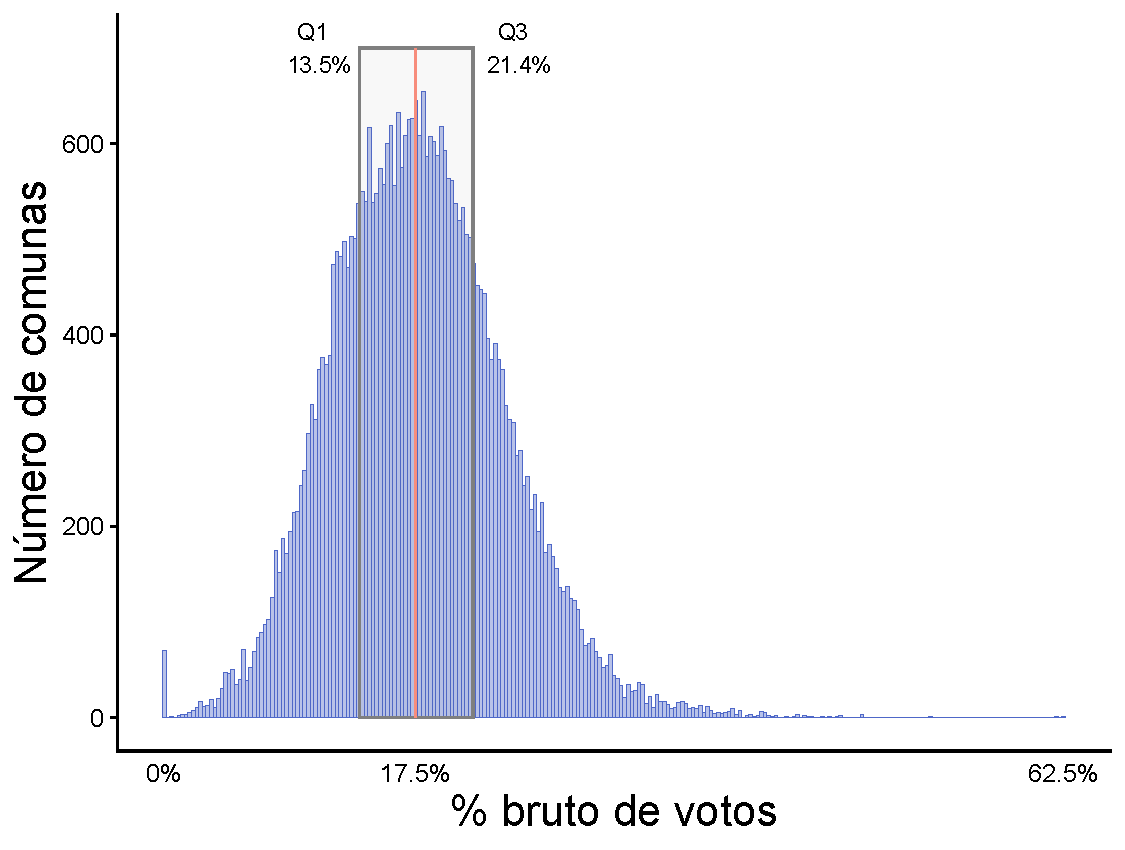
\includegraphics[width = 0.5\textwidth]{Figs/AED/Distr_Votos_Br_P12_FN}
	\caption{Histograma del \% bruto de votos obtenido en cada comuna. Fuente: elaboración propia con base en los datos electorales oficiales del Ministerio del Interior francés.}
	\label{fig:Distr_Br}	
\end{figure}

Podemos agregar los datos a nivel región como en la \textbf{Figura \ref{fig:Pct_Br_Reg_P12}}, para describir de manera más general las zonas de fortaleza o debilidad. Mientras que el porcentaje de votos brutos en la metrópoli fue de 14.6\%, en la región île de France Marine Le Pen obtuvo el 9.4\% y en Picardie llegó a obtener casi el 20\%.\\

Otra forma de valorar la presencia territorial del partido es considerar las comunas de cada región y comparar su distribución frente a la distribución agregada de toda la metrópoli. Podemos ver este ejercicio mediante el \textit{geofacet} de la \textbf{Figura \ref{fig:Geofacet_Distr_Reg_P12}}. Dentro de él comparo los histogramas de los porcentajes de votos que recibió la candidata frontista en las comunas de cada región con la distribución de los porcentajes para todas las comunas de la metrópoli. La intensidad del color de los histogramas depende del cociente del porcentaje mediano de votos en la región entre el porcentaje mediano de votos en toda la metrópoli, por lo que representa la fuerza relativa de cada etiqueta en la región. En azules encontramos las regiones con medianas superiores a la nacional y en rosas a aquellos con menores.\\

\begin{figure}[h]
	\centering
	\begin{subfigure}{0.425\textwidth}
	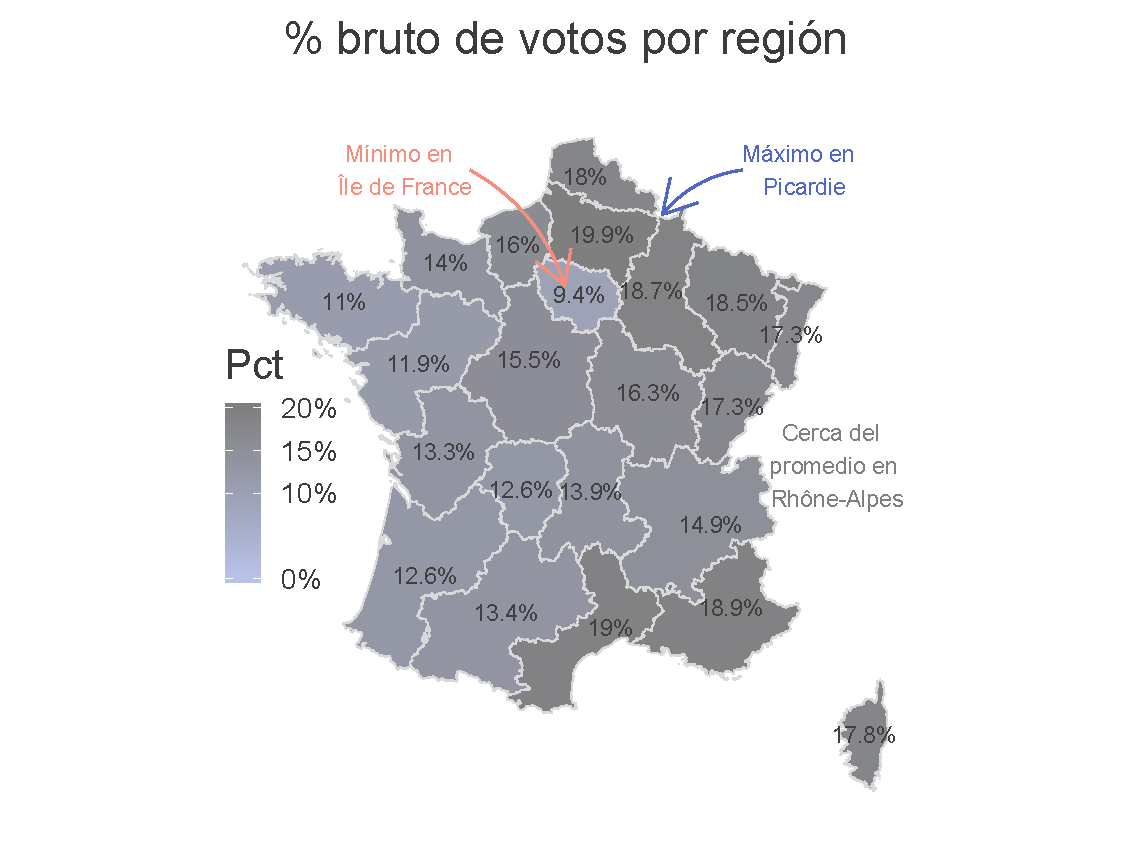
\includegraphics[width = \textwidth]{Figs/AED/Pct_Br_Reg_P12_FN}
	\caption{Mapa del \% bruto de votos obtenido por Marine Le Pen en las elecciones presidenciales del 2012 en cada región francesa.}
	\label{fig:Pct_Br_Reg_P12}		
	\end{subfigure}
	~
	\begin{subfigure}{0.475\textwidth}
	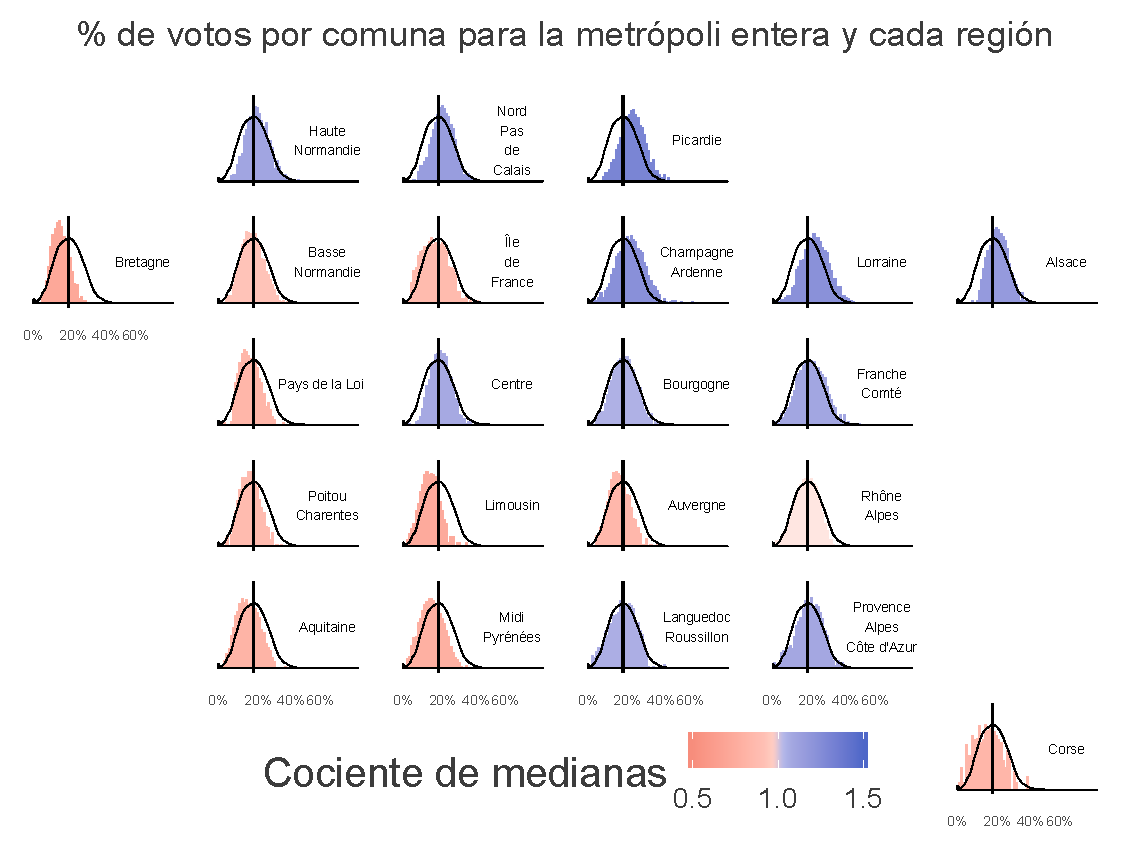
\includegraphics[width = \textwidth]{Figs/AED/Geofacet_Reg_P12_FN}
	\caption{Los histogramas representan la distribución para cada una de las regiones y las densidades la de la metrópoli francesa.}
	\label{fig:Geofacet_Distr_Reg_P12}
	\end{subfigure}
	\caption{Fuente: elaboración propia con base en los datos electorales oficiales del Ministerio del Interior francés y la cartografía de OpenStreetMap.}
\end{figure}

Vemos que, en las regiones del noreste francés como Picardie o Alsace, los histogramas del FN están desplazados hacia la parte derecha de la distribución de referencia y, por tanto, están coloreados con mayor intensidad de azul. Por el contrario, en regiones occidentales como Bretagne, Limousin o Aquitaine, los histogramas reflejan menores porcentajes de votos para el FN y se colorean más de rosa. Podemos empezar a conjeturar que una clave geográfica para el voto frontista es la diagonal que va de Normandía--- Haute y Basse Normandie--- hacia PACA\footnote{Provence-Alpes-Côtes d'Azur.}: si la comuna se encuentra al noreste de la diagonal, tendería a manifestar mayor apoyo al Front National que si se encuentra al sudoeste de la misma. Este sería a grandes rasgos el eje que \textcite{Goodliffe16} identifica como la línea que une las ciudades de Cherbourg en Normandía y Valence en Rhône-Alpes y después con Perpignan en Languedoc-Rousillon.\\ 

Si descendemos un nivel y observamos el mapa a nivel departamento en la \textbf{Figura \ref{fig:Pct_Br_Dptos_P12}}, la división este-oeste se ve de manera más clara. También podemos ver las distribuciones a nivel departamento mediante diagramas de violines. El \textit{geofacet} respectivo se observa en la \textbf{Figura \ref{fig:Geofacet_Distr_Dptos_P12}}. En cada región se muestran 3 líneas como referencia de los tres cuartiles considerando las comunas de toda la metrópoli. El diagrama de violín sin relleno muestra dicha distribución agrupada para toda la metrópoli. Los diagramas de violín con relleno representan, pues, las distribuciones del porcentaje de votos obtenido en cada comuna del departamento correspondiente, identificado mediante su código oficial geográfico. Dentro de cada región los departamentos están ordenados de menor a mayor apoyo al FN con base en las medianas. Al igual que en los histogramas a nivel región, la intensidad del relleno es el cociente de la mediana departamental respecto a la mediana global.\\ 

\begin{figure}[h]
	\centering
	\begin{subfigure}{0.4\textwidth}
	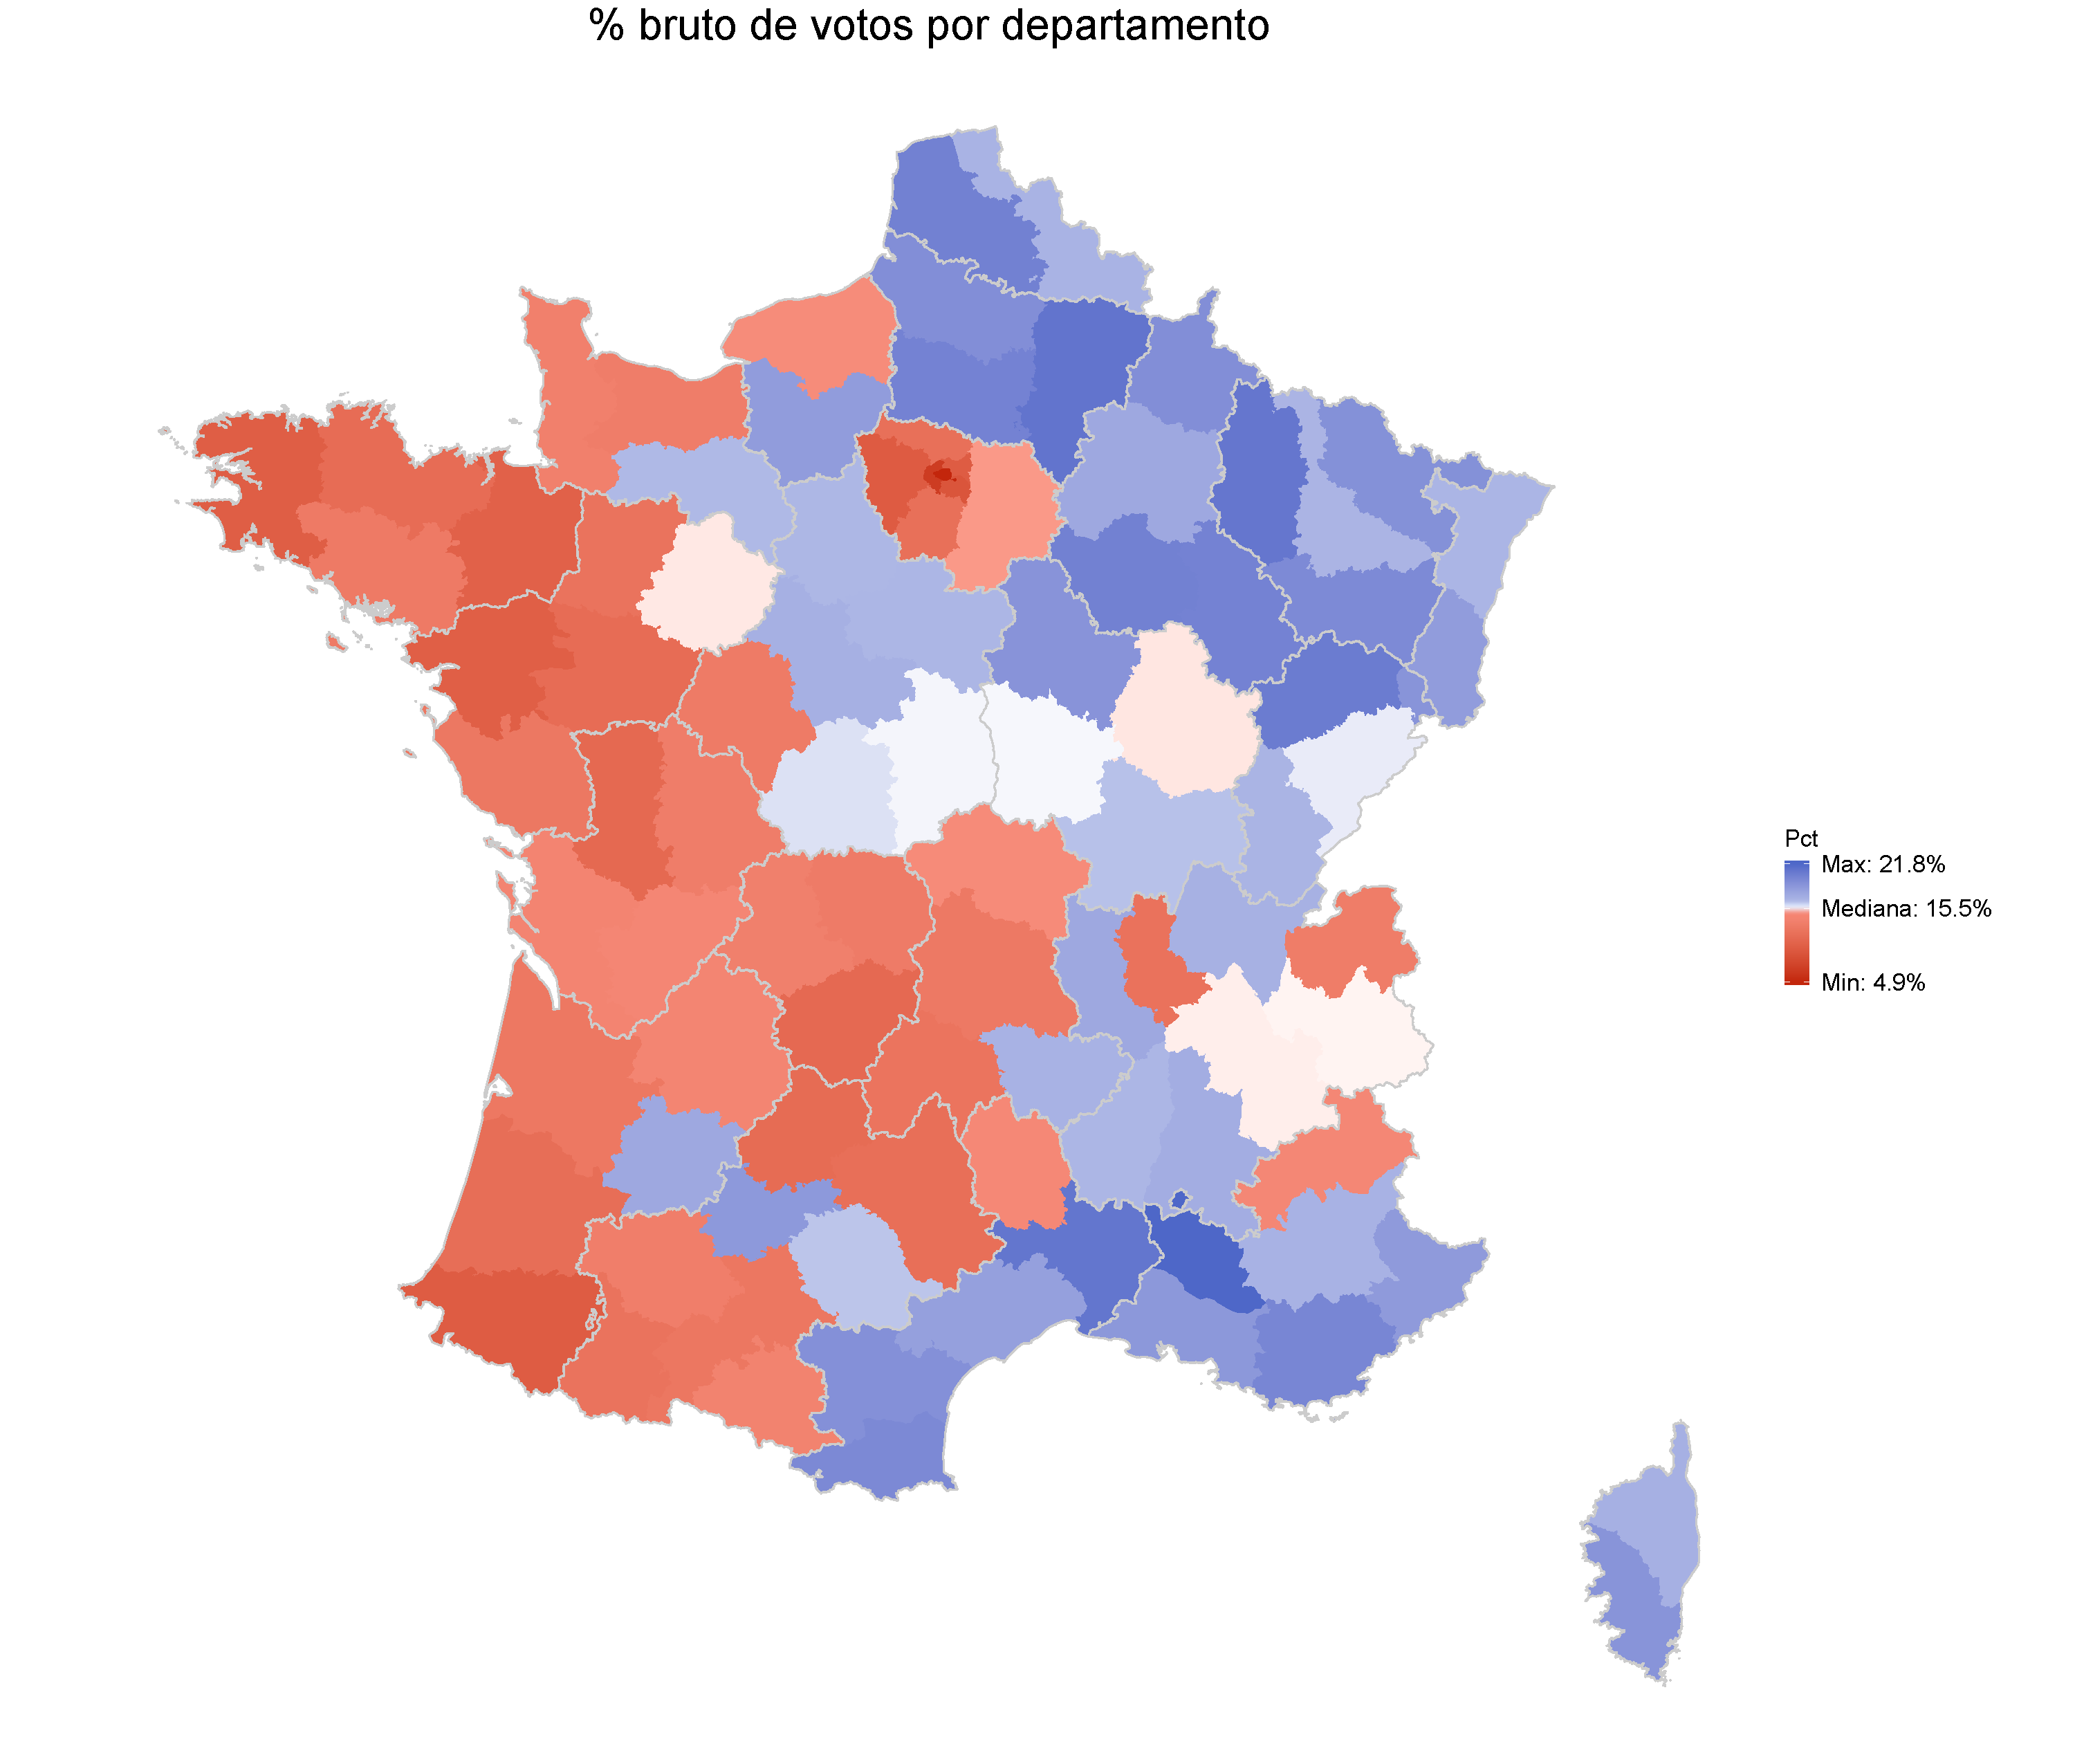
\includegraphics[width = \textwidth]{Figs/AED/Mapa_Dptos_Br_P12_FN}
	\caption{Mapa del \% bruto de votos obtenido por Marine Le Pen en las elecciones presidenciales del 2012 en cada departamento.}
	\label{fig:Pct_Br_Dptos_P12}	
	\end{subfigure}
	~
	\begin{subfigure}{0.5\textwidth}
	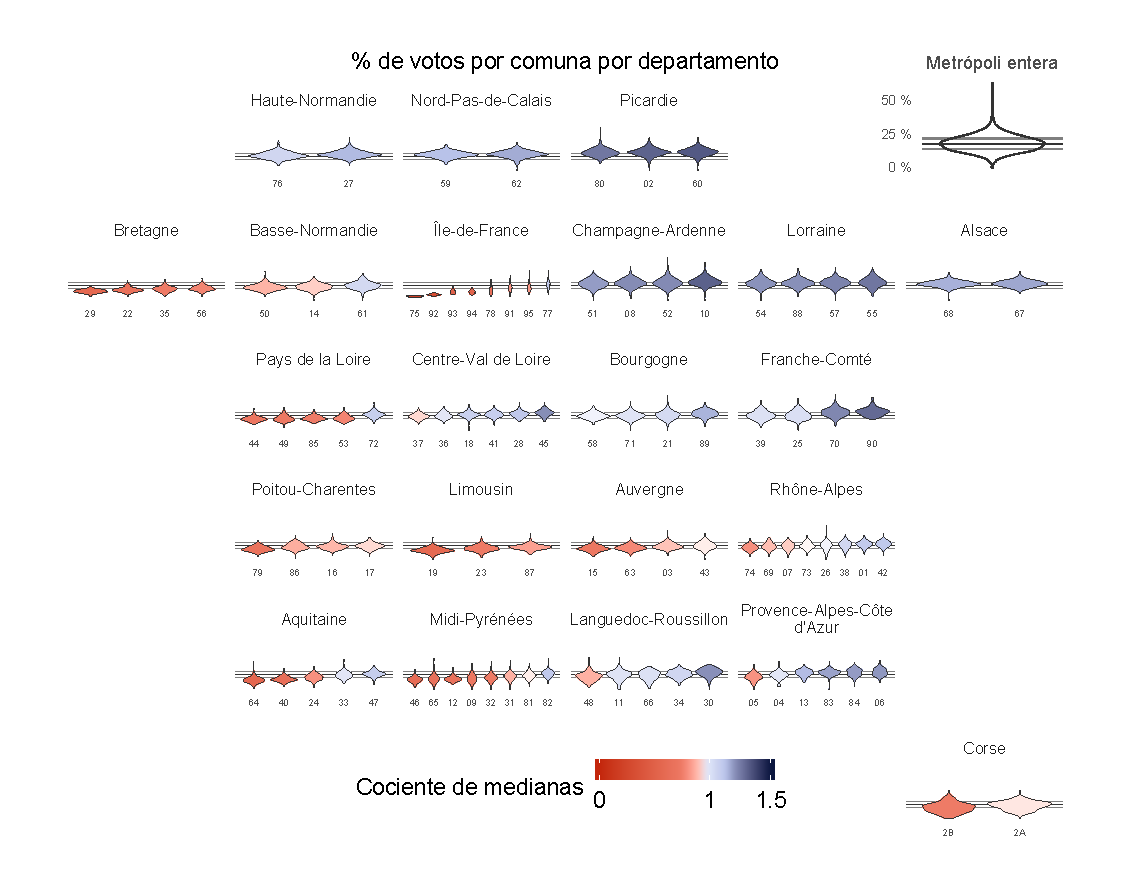
\includegraphics[width = \textwidth]{Figs/AED/Geofacet_Dpto_P12_FN}
	\caption{Los violines rellenos de color son las distribuciones dentro del departamento correspondiente mientras que las 3 líneas horizontales representan una referencia al rango intercuartílico y la mediana considerando todas las comunas de la metrópoli, cuya distribución puede verse en el panel superior derecho.}
	\label{fig:Geofacet_Distr_Dptos_P12}	
	\end{subfigure}
	\caption{Fuente: elaboración propia con base en los datos electorales oficiales del Ministerio del Interior francés y la cartografía de OpenStreetMap.}
\end{figure}

Dentro de las regiones con mayor apoyo en general, este es relativamente homogéneo a través de los departamentos. En efecto, las distribuciones reflejadas en diagramas de violines para los departamentos dentro de Lorraine, Champagne-Ardenne o Picardie aparentan ser similares, siempre con cocientes de medianas mayores a 1. No obstante, existen regiones--- como Île de France o Aquitaine--- cuyos departamentos presentan distribuciones más variables. Este es un elemento que podría empezar a sugerir un modelado jerárquico de los datos por departamento.\\

Finalmente, observamos el mapa de los porcentajes de voto brutos que obtuvo Marine Le Pen en cada comuna en la \textbf{Figura \ref{fig:Mapa_Pct_Br}}. De nueva cuenta distinguimos zonas de fuerza o debilidad con respecto a la mediana. Es decir, en tonos de azul se encuentran la mitad de las comunas con mayor porcentaje de votos y en rojos la mitad de menor porcentaje. La variabilidad es clara. Observamos lo que autores como \textcite{LeBras15} llaman las capas del voto FN. En primer lugar la gran zona de fuerza del norte. También hay corredores de fortaleza: el litoral mediterráneo y dos diagonales que parecen desembocar en él; estas serían las márgenes del Ródano que viene del norte y del Garona que viene del Atlántico. La débilidad la encontramos al oeste y en zonas urbanas vistas como manchas rojas rodeadas de color azul, particularmente París.

\begin{figure}[h]
	\centering
	\includegraphics[width = 0.5\textwidth]{Figs/AED/Mapa_Votos_Br_P12_FN}
	\caption{Mapa del \% bruto de votos obtenido por Marine Le Pen en las elecciones presidenciales del 2012. Fuente: elaboración propia con base en los datos electorales oficiales del Ministerio del Interior francés y la cartografía de OpenStreetMap.}
	\label{fig:Mapa_Pct_Br}	
\end{figure}

\section{Datos censales}

Por otro lado, para caracterizar a las comunas en términos de \textit{configuraciones sociales} relacionadas con el voto nativista y autoritario de corte populista, requerimos su composición en términos de variables sociodemográficas. Afortunadamente, desde 2004, Francia cuenta con un sistema censal rotante que permite realizar estimaciones anuales para este tipo de variables.\\ 

De acuerdo con el \textcite{FichaCenso}, el censo francés está compuesto por dos mecanismos distintos dependiendo del tamaño poblacional de la comuna. La comunas de menos de 10,000 habitantes realizan una encuesta censal a razón de una de cada cinco comunas todos los años. Las comunas de 10,000 habitantes o más realizan todos los años una encuesta por muestreo probabilístico del 8\% de sus hogares cada año. Acumulando cinco años, el total de los habitantes de las comunas ``pequeñas'' y al rededor del 40\% de la población de las comunas ``grandes'' son tomados en cuenta. Esta muestra acumulada se trata de manera estadística para estimar la población total en cada comuna al tercer año de una ventana de cinco. Así, para la estimación de la población al año $n$ se consideran los datos de los años $n-2$, $n-1$, $n$, $n+1$ y $n+2$. Cada año se desecha la información más antigua y se incorpora la información del nuevo año.  La primera estimación anual se tuvo en 2006 considerando la información de 2004 a 2008.\\

A partir de estos datos oficiales anuales que publica el INSEE podemos descomponer las distribuciones poblacionales en las comunas francesas respecto a algunas variables que la revisión de literatura sugiere como explicativas: las categorías socioprofesionales, nacionalidad o condición migratoria, sexo y edad. Para ello he calculado el porcentaje de individuos como proporción de la población comunal de cada categoría dentro de estas 5 variables sociodemográficas básicas provenientes de 3 bases de datos distintas que se pueden ver en el \textbf{Cuadro \ref{tbl:Variables_Censales}}.\\ 

\begin{table}[h]
\centering
\resizebox{\linewidth}{!}{
\begin{tabular}{|c | c | c | c |}
\hline
\textbf{Base de origen} &
\textbf{Variable} & 
\textbf{Abreviatura} & 
\textbf{Categoría}\\[2pt] 
\hline
\multirow{8}{*}{POB1B} & 
\multirow{2}{*}{Sexo} &  
Hom & Hombres\\ 
&& Muj & Mujeres \\ \cline{2-4}
& \multirow{6}{*}{Edad} & 
Ed1 & 0 a 17 años\\ 
&& Ed2 & 18 a 24 años\\  
&& Ed3 & 25 a 39 años\\  
&& Ed4 & 40 a 54 años\\ 
&& Ed5 & 55 a 64 años\\  
&& Ed6 & 65+ años\\ \hline
\multirow{10}{*}{NAT3A} & 
\multirow{2}{*}{Nacionalidad} & 
Fra & Franceses\\
&& Ext & Extranjeros\\ \cline{2-4}
& \multirow{8}{*}{Categoría Socioprofesional} & 
CSP1 & Agricultores\\
&& CSP2 & Artesanos, comerciantes y empresarios\\
&& CSP3 & Cuadros y profesiones intelectuales superiores\\
&& CSP4 & Profesiones intermediarias\\
&& CSP5 & Empleados\\
&& CSP6 & Obreros\\
&& CSP7 & Retirados\\
&& CSP8 & Otras personas sin actividad\\ \hline
\multirow{2}{*}{IMG1A} & 
\multirow{2}{*}{Condición migratoria} & 
Inm & Inmigrantes\\
&& Loc & Locales\\ \hline
\end{tabular}
}
\caption{Variables censales del INSEE a utilizar en el análisis.}
\label{tbl:Variables_Censales}
\end{table}

 Debido a que las variables de Sexo, Nacionalidad e Inmigración cuentan con dos categorías, solo presento las distribuciones de una categoría de referencia, pues la otra solo es el complemento de esta.\\

Comenzando con la distribución del porcentaje de Mujeres en las comunas en 2012 vemos que, como es de esperarse, la mayoría de los departamentos tienen distribuciones muy concentradas al rededor del 50\% de la población. Las únicas distribuciones que llaman la atención en la \textbf{Figura \ref{fig:Distr_por_Dpto_Muj_2012}} son las de los departamentos de Île de France, con porcentajes un poco mayores que el resto de la metrópoli.\\ 

\begin{figure}[h]
	\centering
	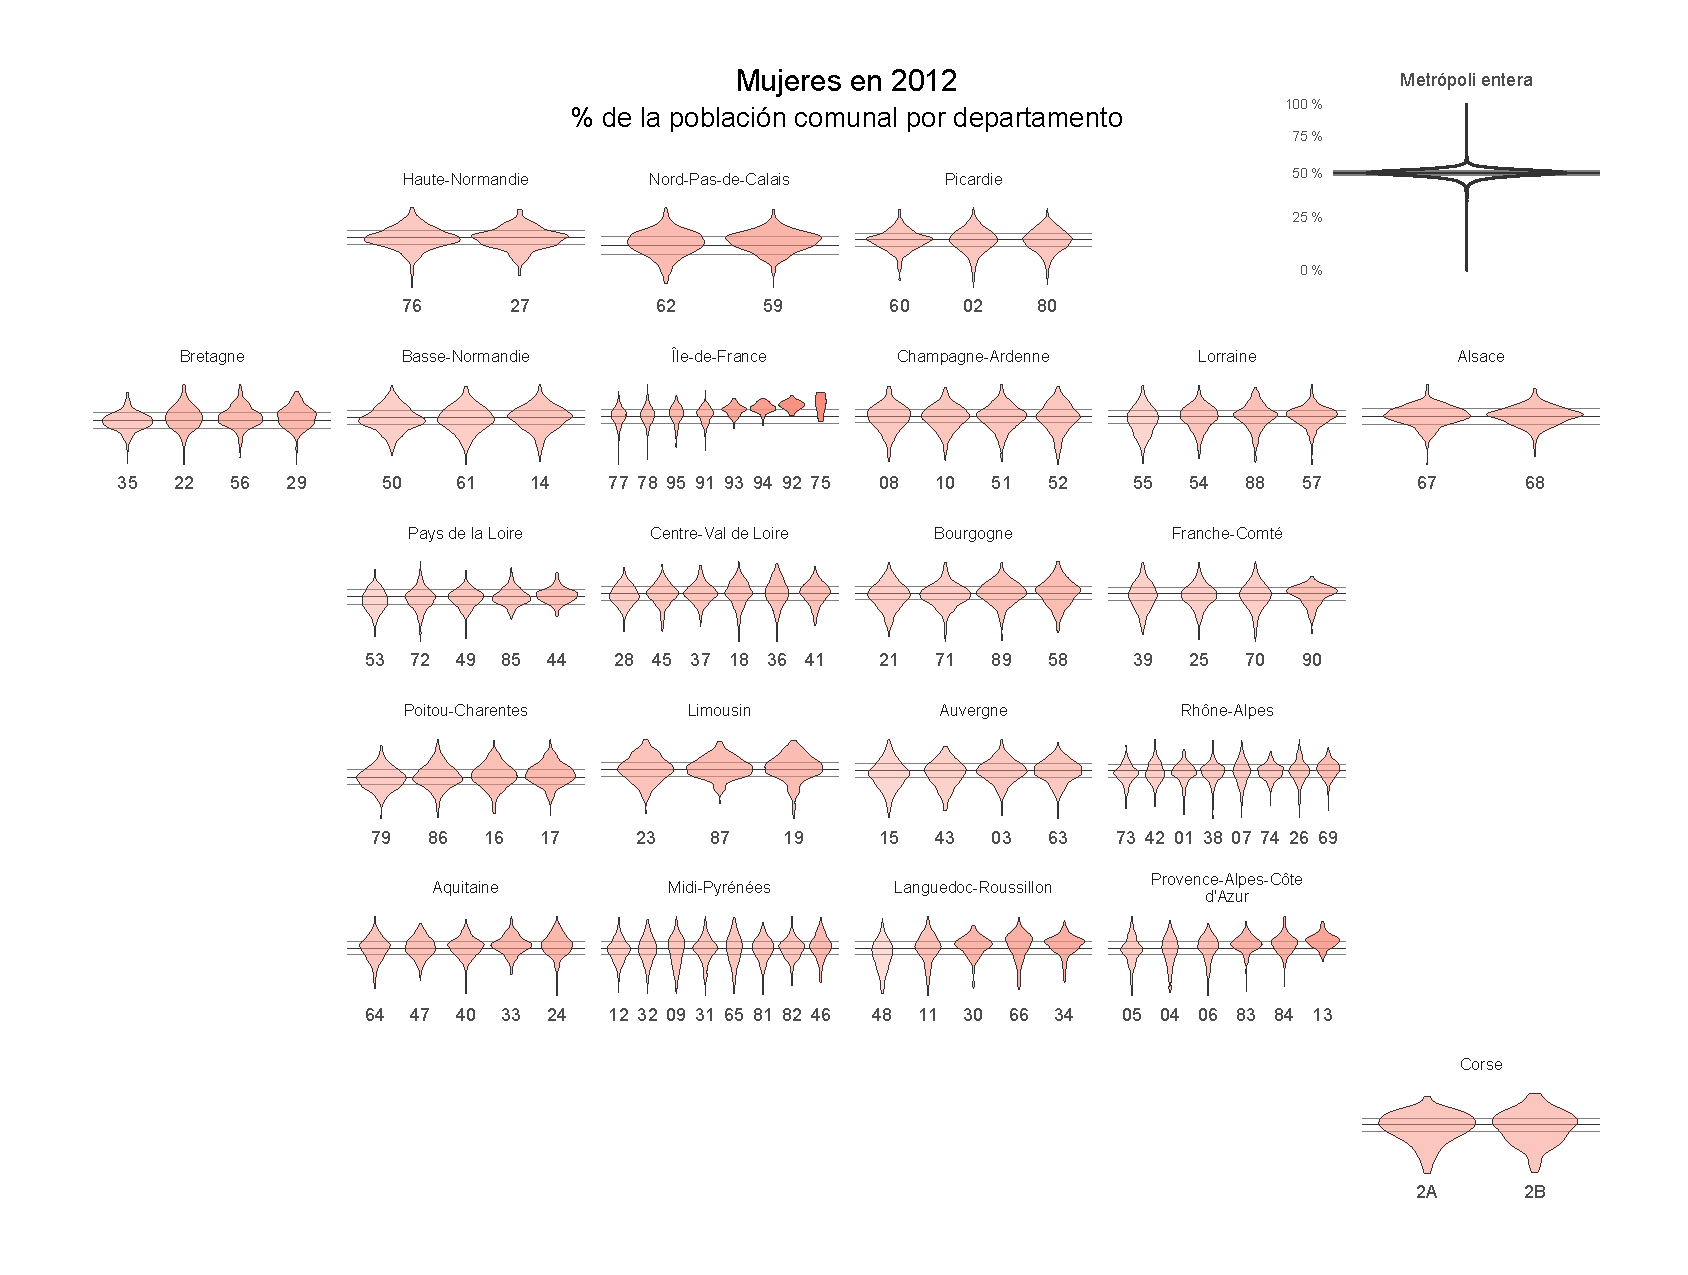
\includegraphics[width = 0.45\textwidth]{Figs/AED/Geofacet_Distr_por_Dpto_Muj_2012}
	\caption{Distribuciones departamentales del porcentaje de mujeres como proporción de la población de las comunas en 2012. Fuente: elaboración propia con los datos censales.}
	\label{fig:Distr_por_Dpto_Muj_2012}	
\end{figure}

Las variables de nacionalidad y condición migratoria son similares pero no idénticas. El \textcite{DefsCenso} define a un extranjero como un residente del territorio francés que no posee la nacionalidad francesa y a un inmigrante como aquella persona nacida extranjera en el extranjero; esto quiere decir, por ejemplo, que hay individuos franceses considerados inmigrantes pues pudieron haberse naturalizado, así como extranjeros considerados locales porque nacieron en territorio francés sin tener derecho a la nacionalidad.\\ 

En el proceso del modelado se deberá elegir la ``mejor'' de entre ambas. Por el momento, en la \textbf{Figura \ref{fig:Distr_por_Dpto_Nac_Inm_2012}} vemos las distribuciones para los extranjeros y los inmigrantes en 2012. Debido a que la mayoría de inmigrantes son extranjeros las distribuciones siguen un patrón muy parecido, salvo que en general siempre hay más inmigrantes que extranjeros--- observar líneas de referencia---. Mientras que en regiones del norte las comunas tienden a tener pocos extranjeros e inmigrantes, vemos que en la región parisina de Île de France tienen una presencia considerable. Las regiones más sureñas como Corse o PACA también tienen comunas con mayor presencia de extranjeros e inmigrantes.\\

\begin{figure}[h]
	\centering
	\begin{subfigure}{0.45\textwidth}
	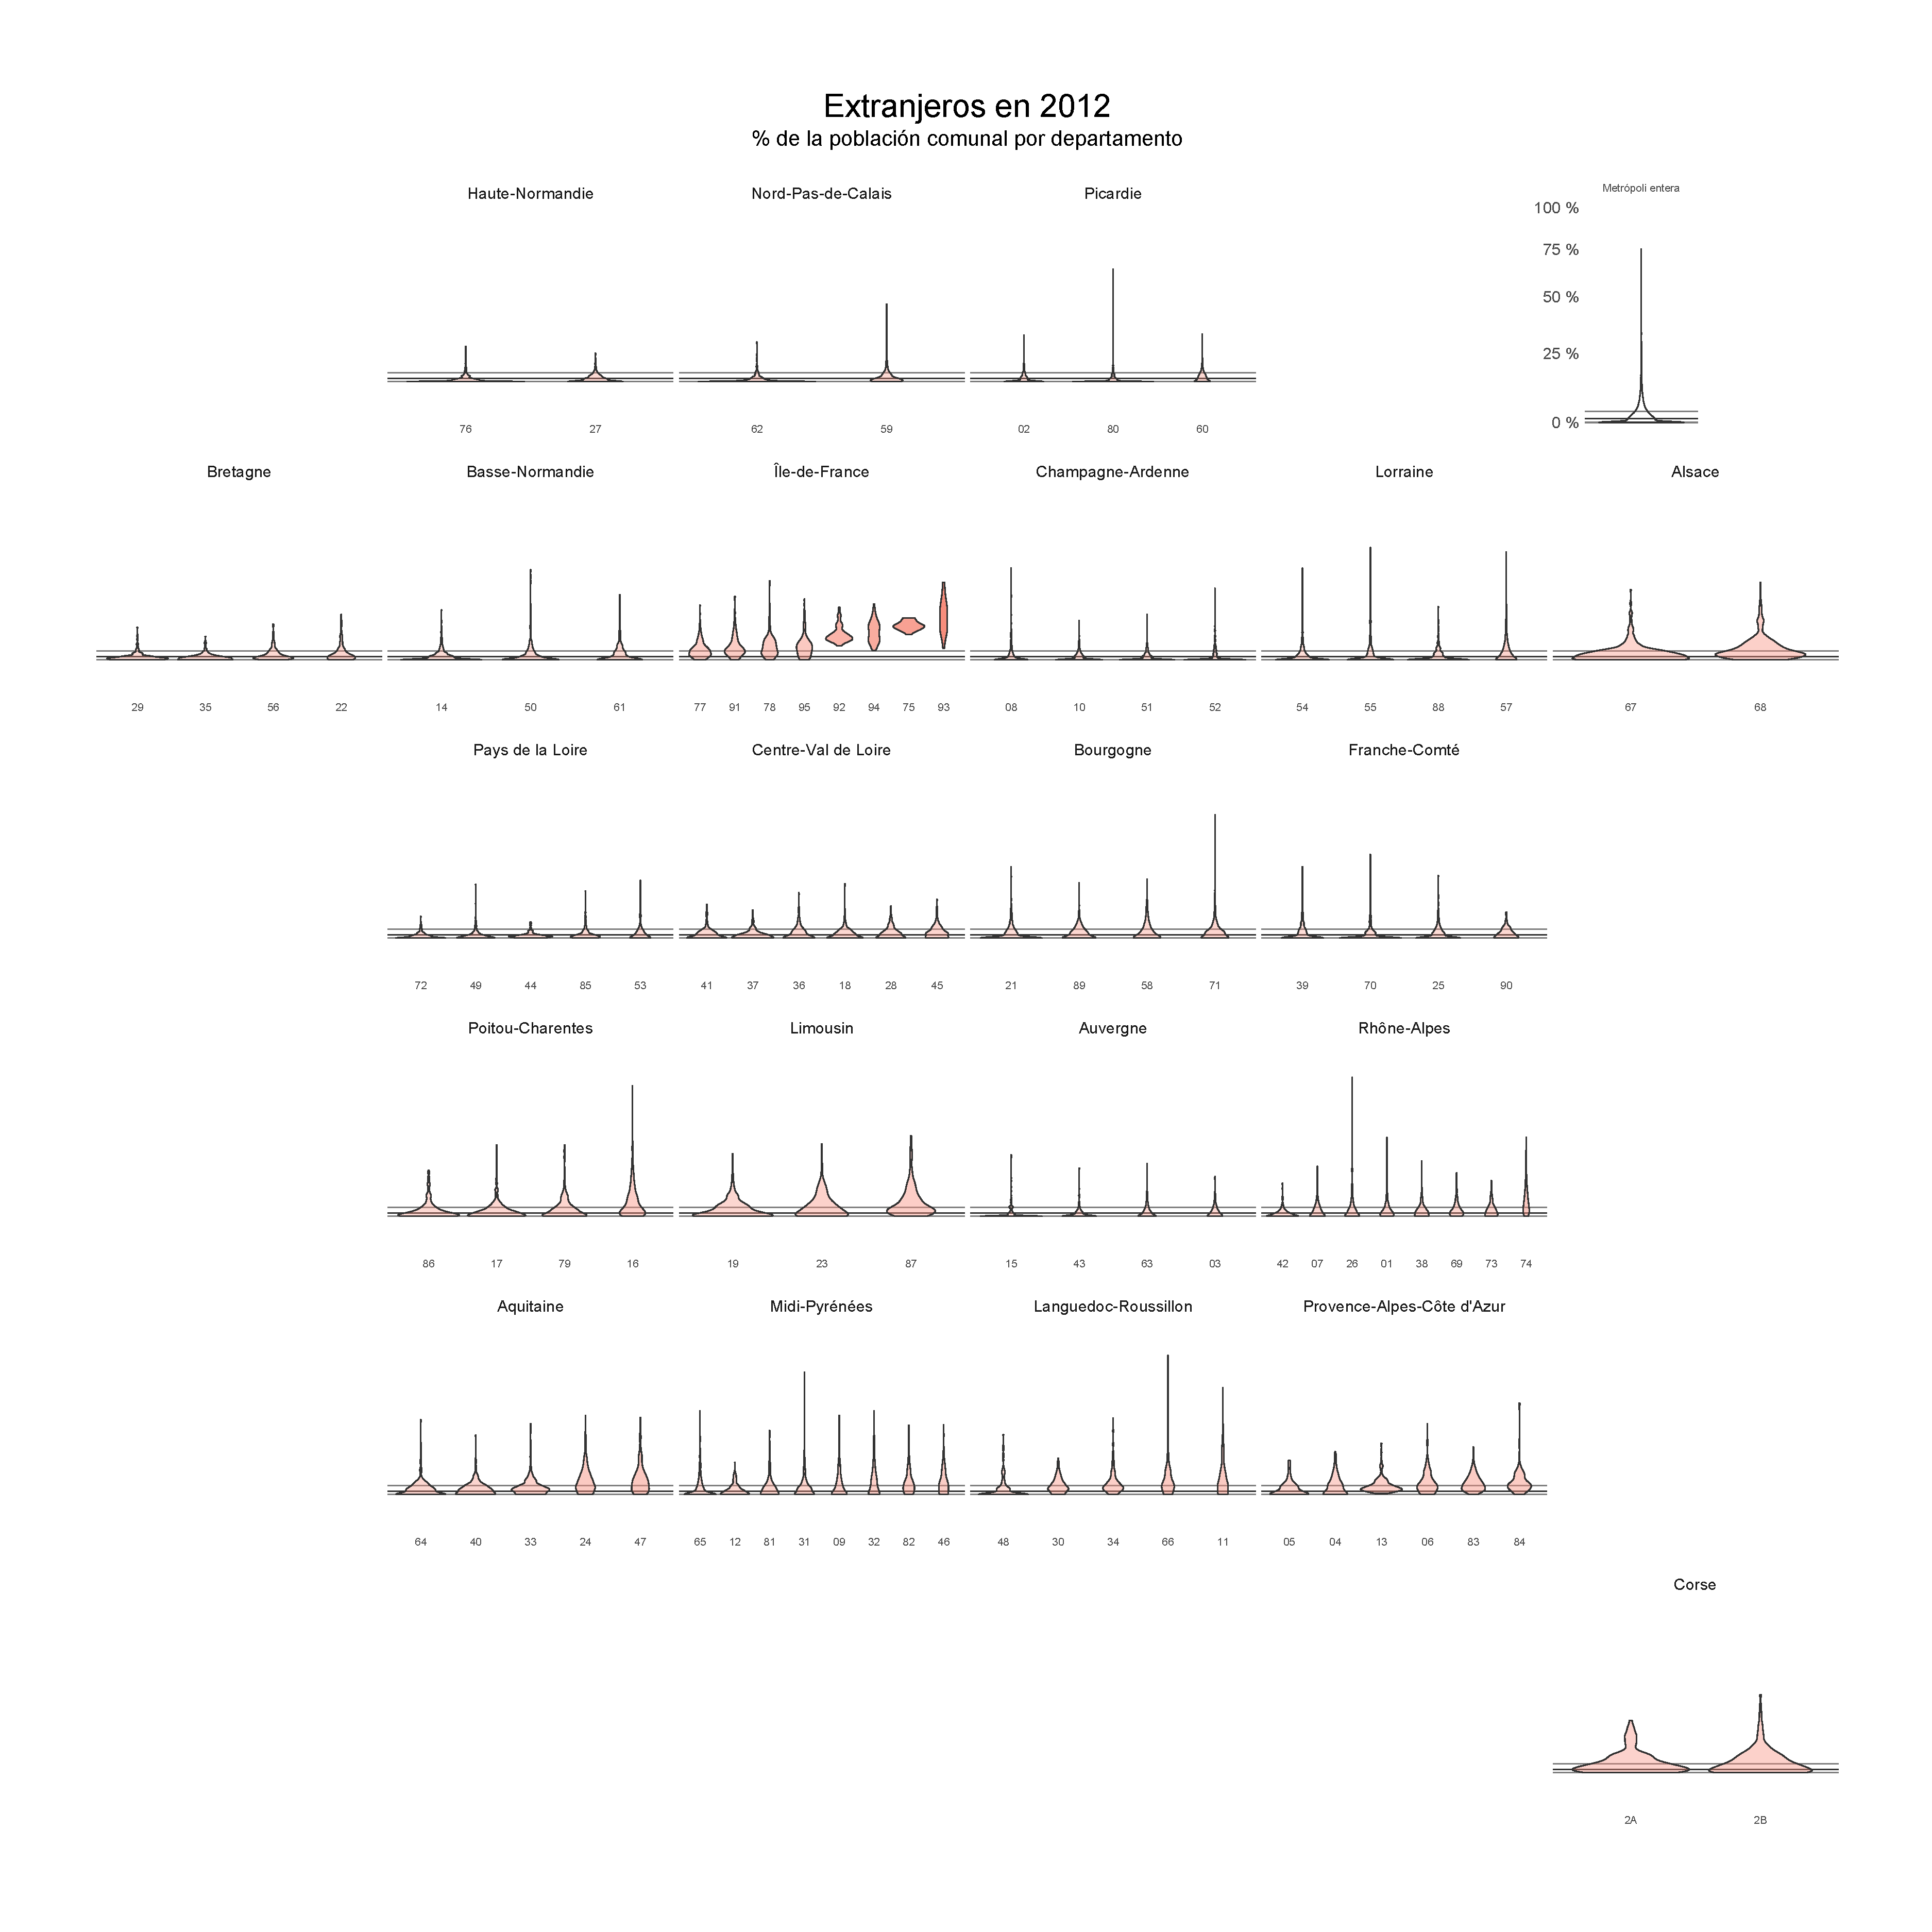
\includegraphics[width = \textwidth]{Figs/AED/Geofacet_Distr_por_Dpto_Ext_2012}
	\end{subfigure}
	~
	\begin{subfigure}{0.45\textwidth}
	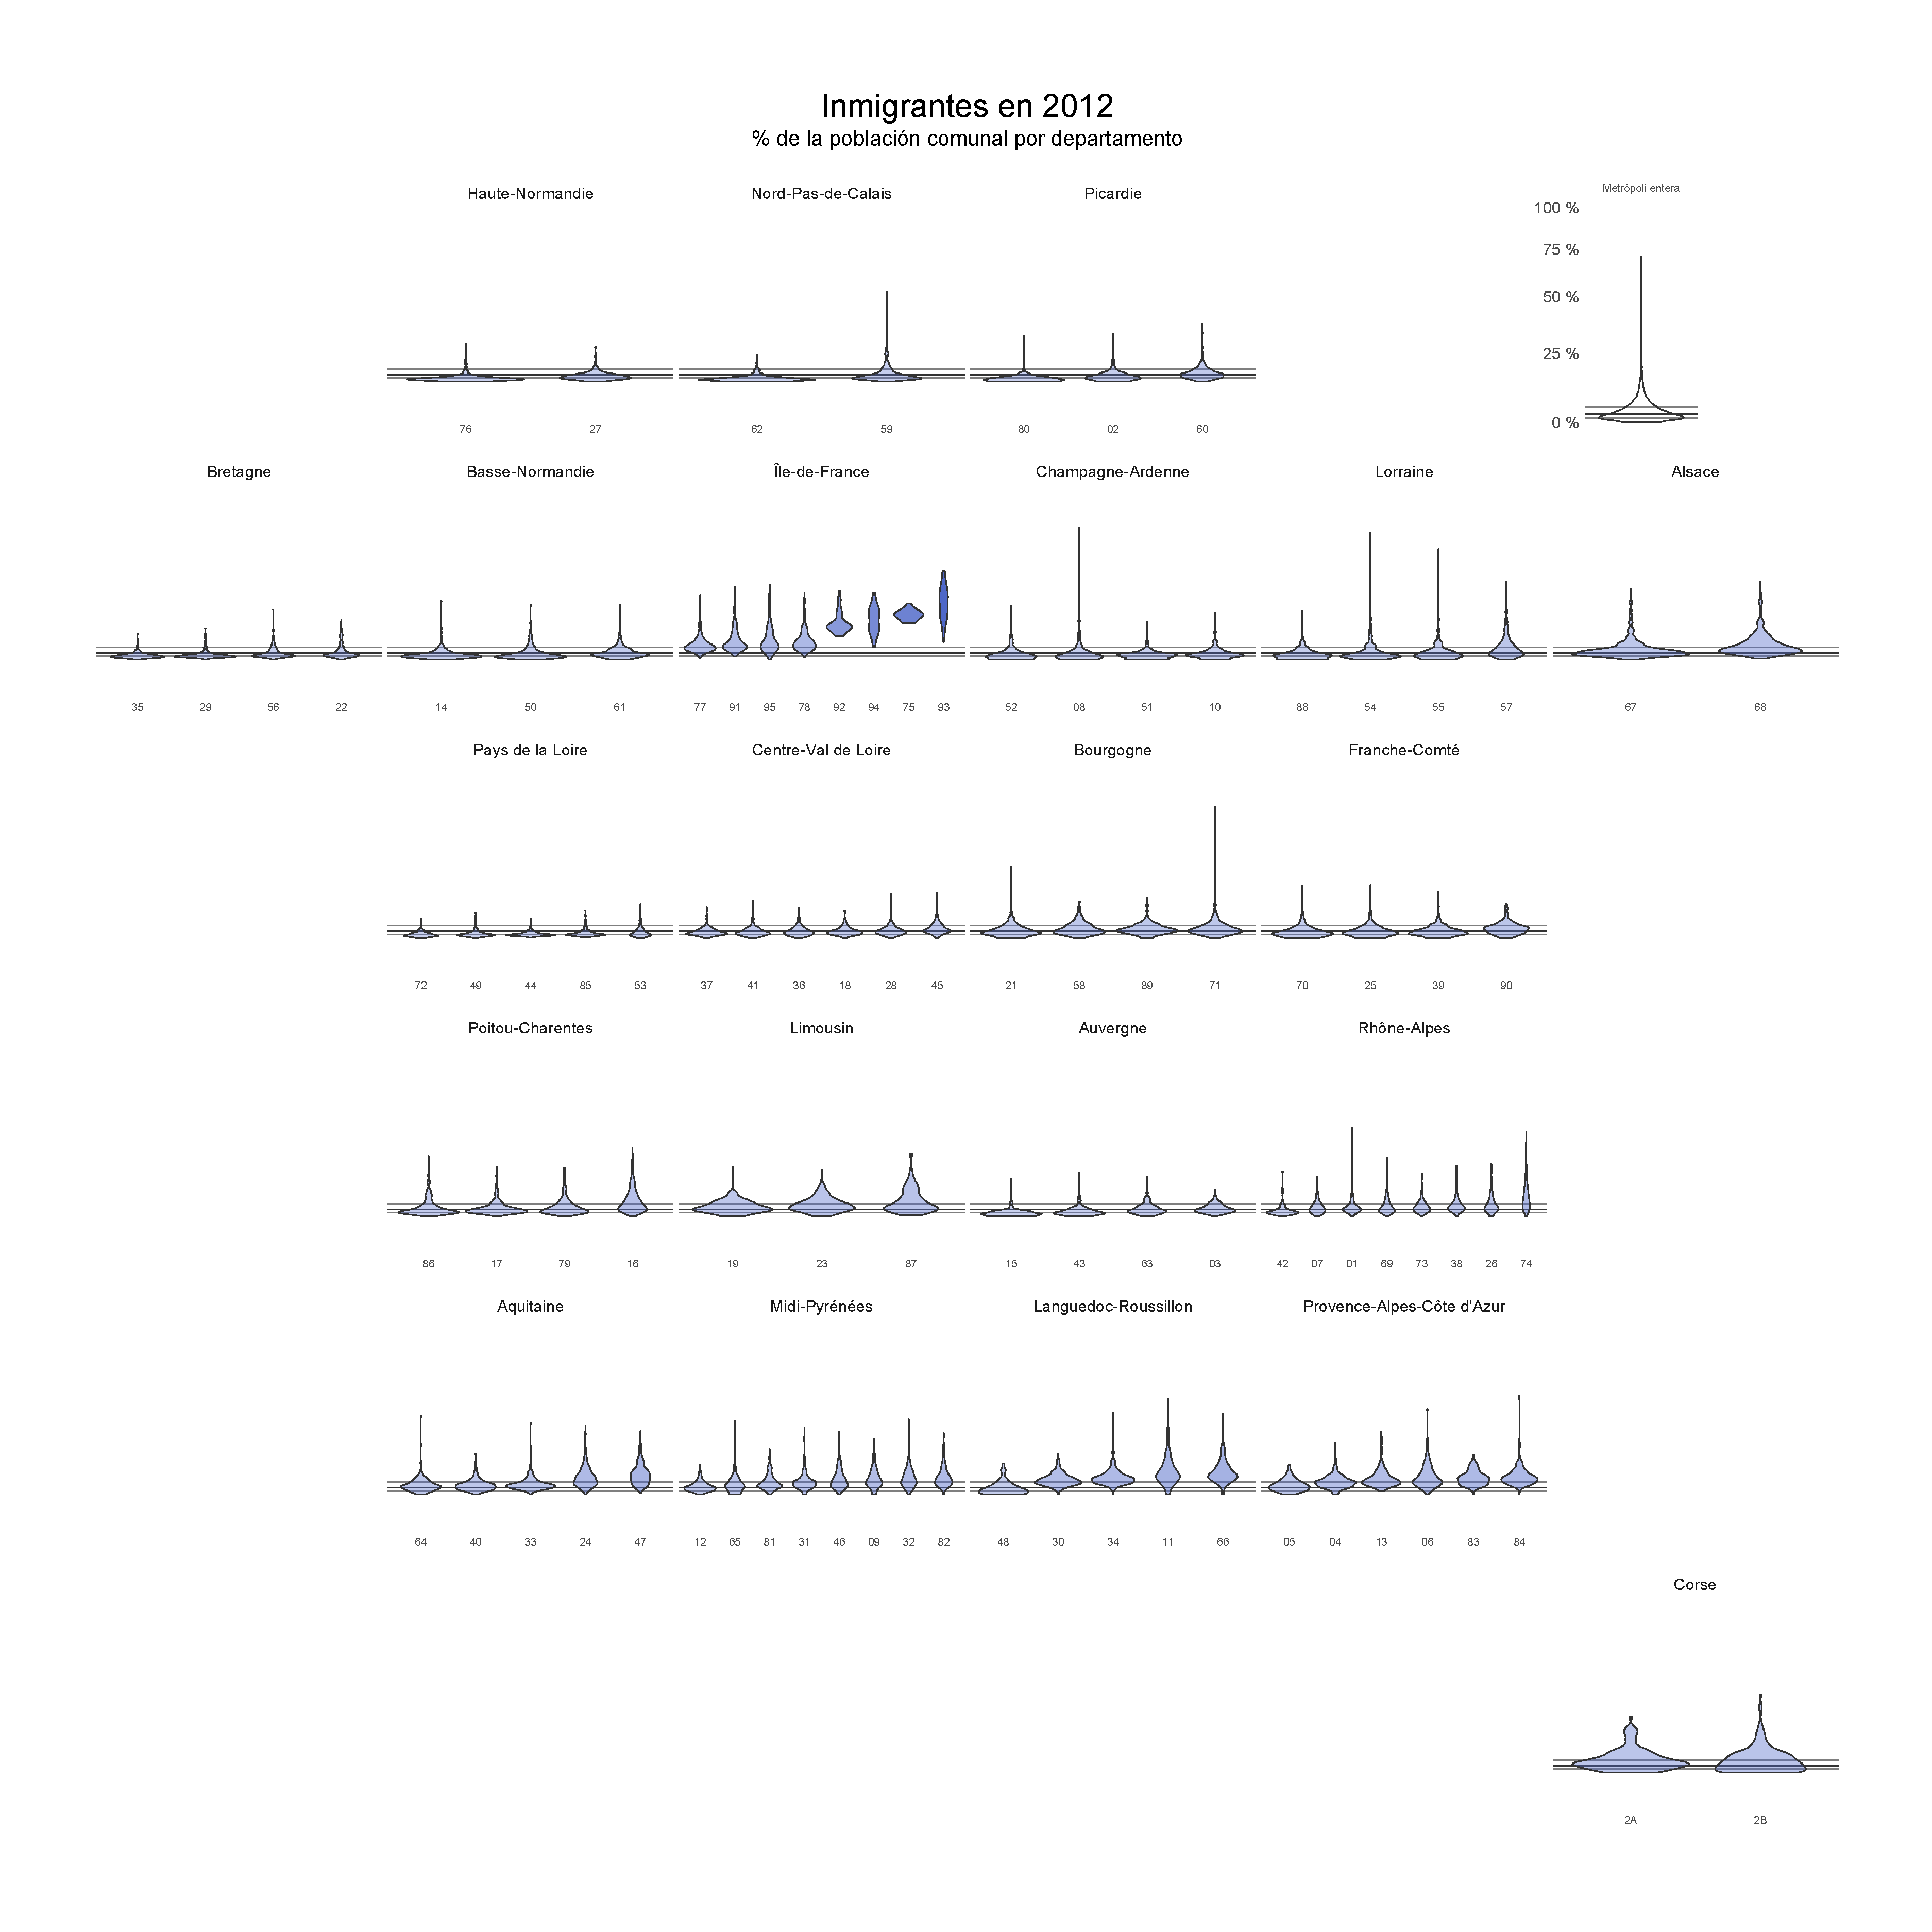
\includegraphics[width = \textwidth]{Figs/AED/Geofacet_Distr_por_Dpto_Inm_2012}
	\end{subfigure}
	\caption{Distribuciones departamentales del porcentaje de extranjeros y de inmigrantes como proporción de la población de las comunas en 2012. Fuente: elaboración propia con los datos censales.}
	\label{fig:Distr_por_Dpto_Nac_Inm_2012}	
\end{figure}

Ahora bien, la estructura generacional de las comunas francesas va cambiando. Si observamos las distribuciones para los diferentes grupos de edad en la \textbf{Figura \ref{fig:Distr_por_Dpto_Edades_2012}} vemos que hay regiones cuyos departamentos tienden a tener comunas más \textit{envejecidas} en el sentido de que hay comparativamente menor porcentaje de menores de edad o jóvenes que en el resto de la metrópoli y mayores porcentajes de personas de 65 años o más. Esto se ve particularmente en Corse, pero también en otras regiones como Limousin, Midi-Pyrinées o Bourgogne. Por el contrario, el norte y particularmente Île de France presentan una estructura generacional más joven.\\

\begin{figure}[h]
	\centering
	\begin{subfigure}{0.3\textwidth}
	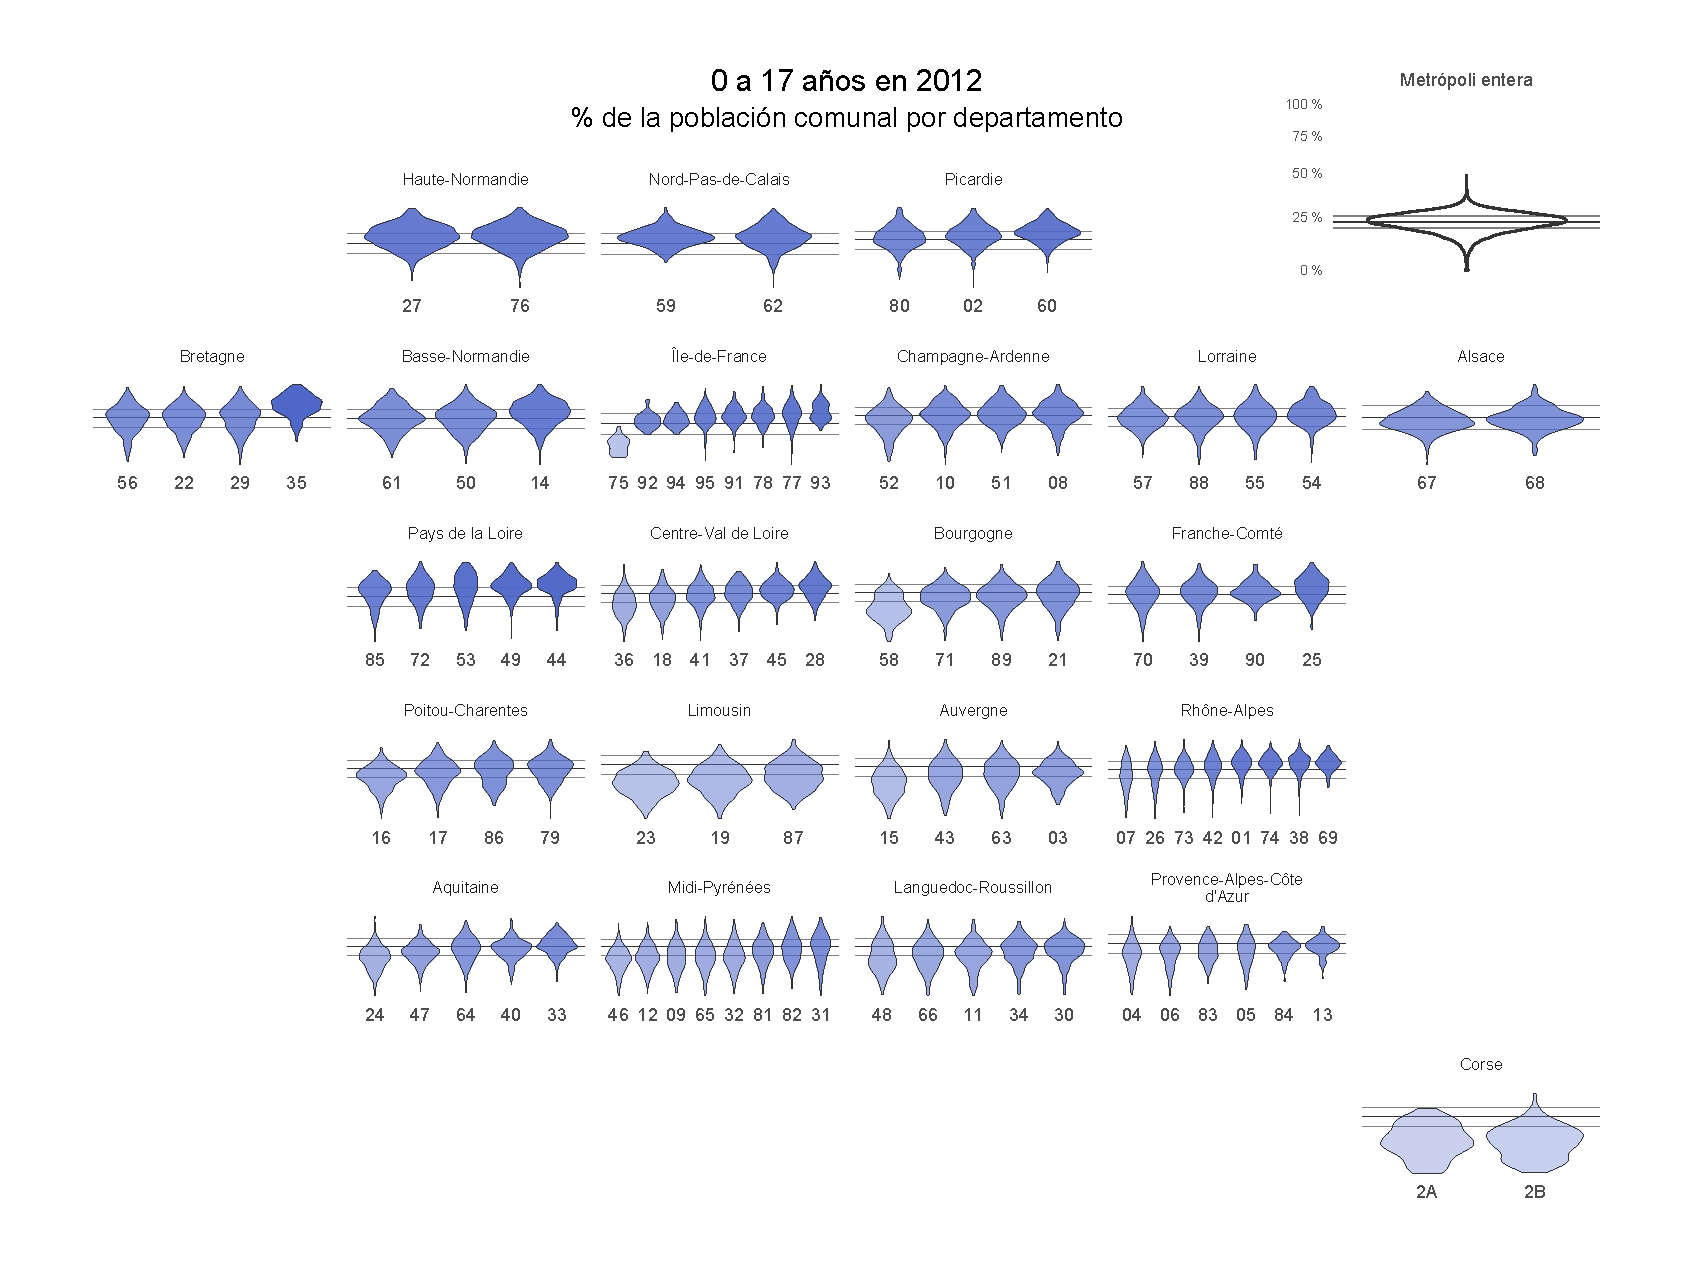
\includegraphics[width = \textwidth]{Figs/AED/Geofacet_Distr_por_Dpto_Ed1_2012}
	\end{subfigure}
	~
	\begin{subfigure}{0.3\textwidth}
	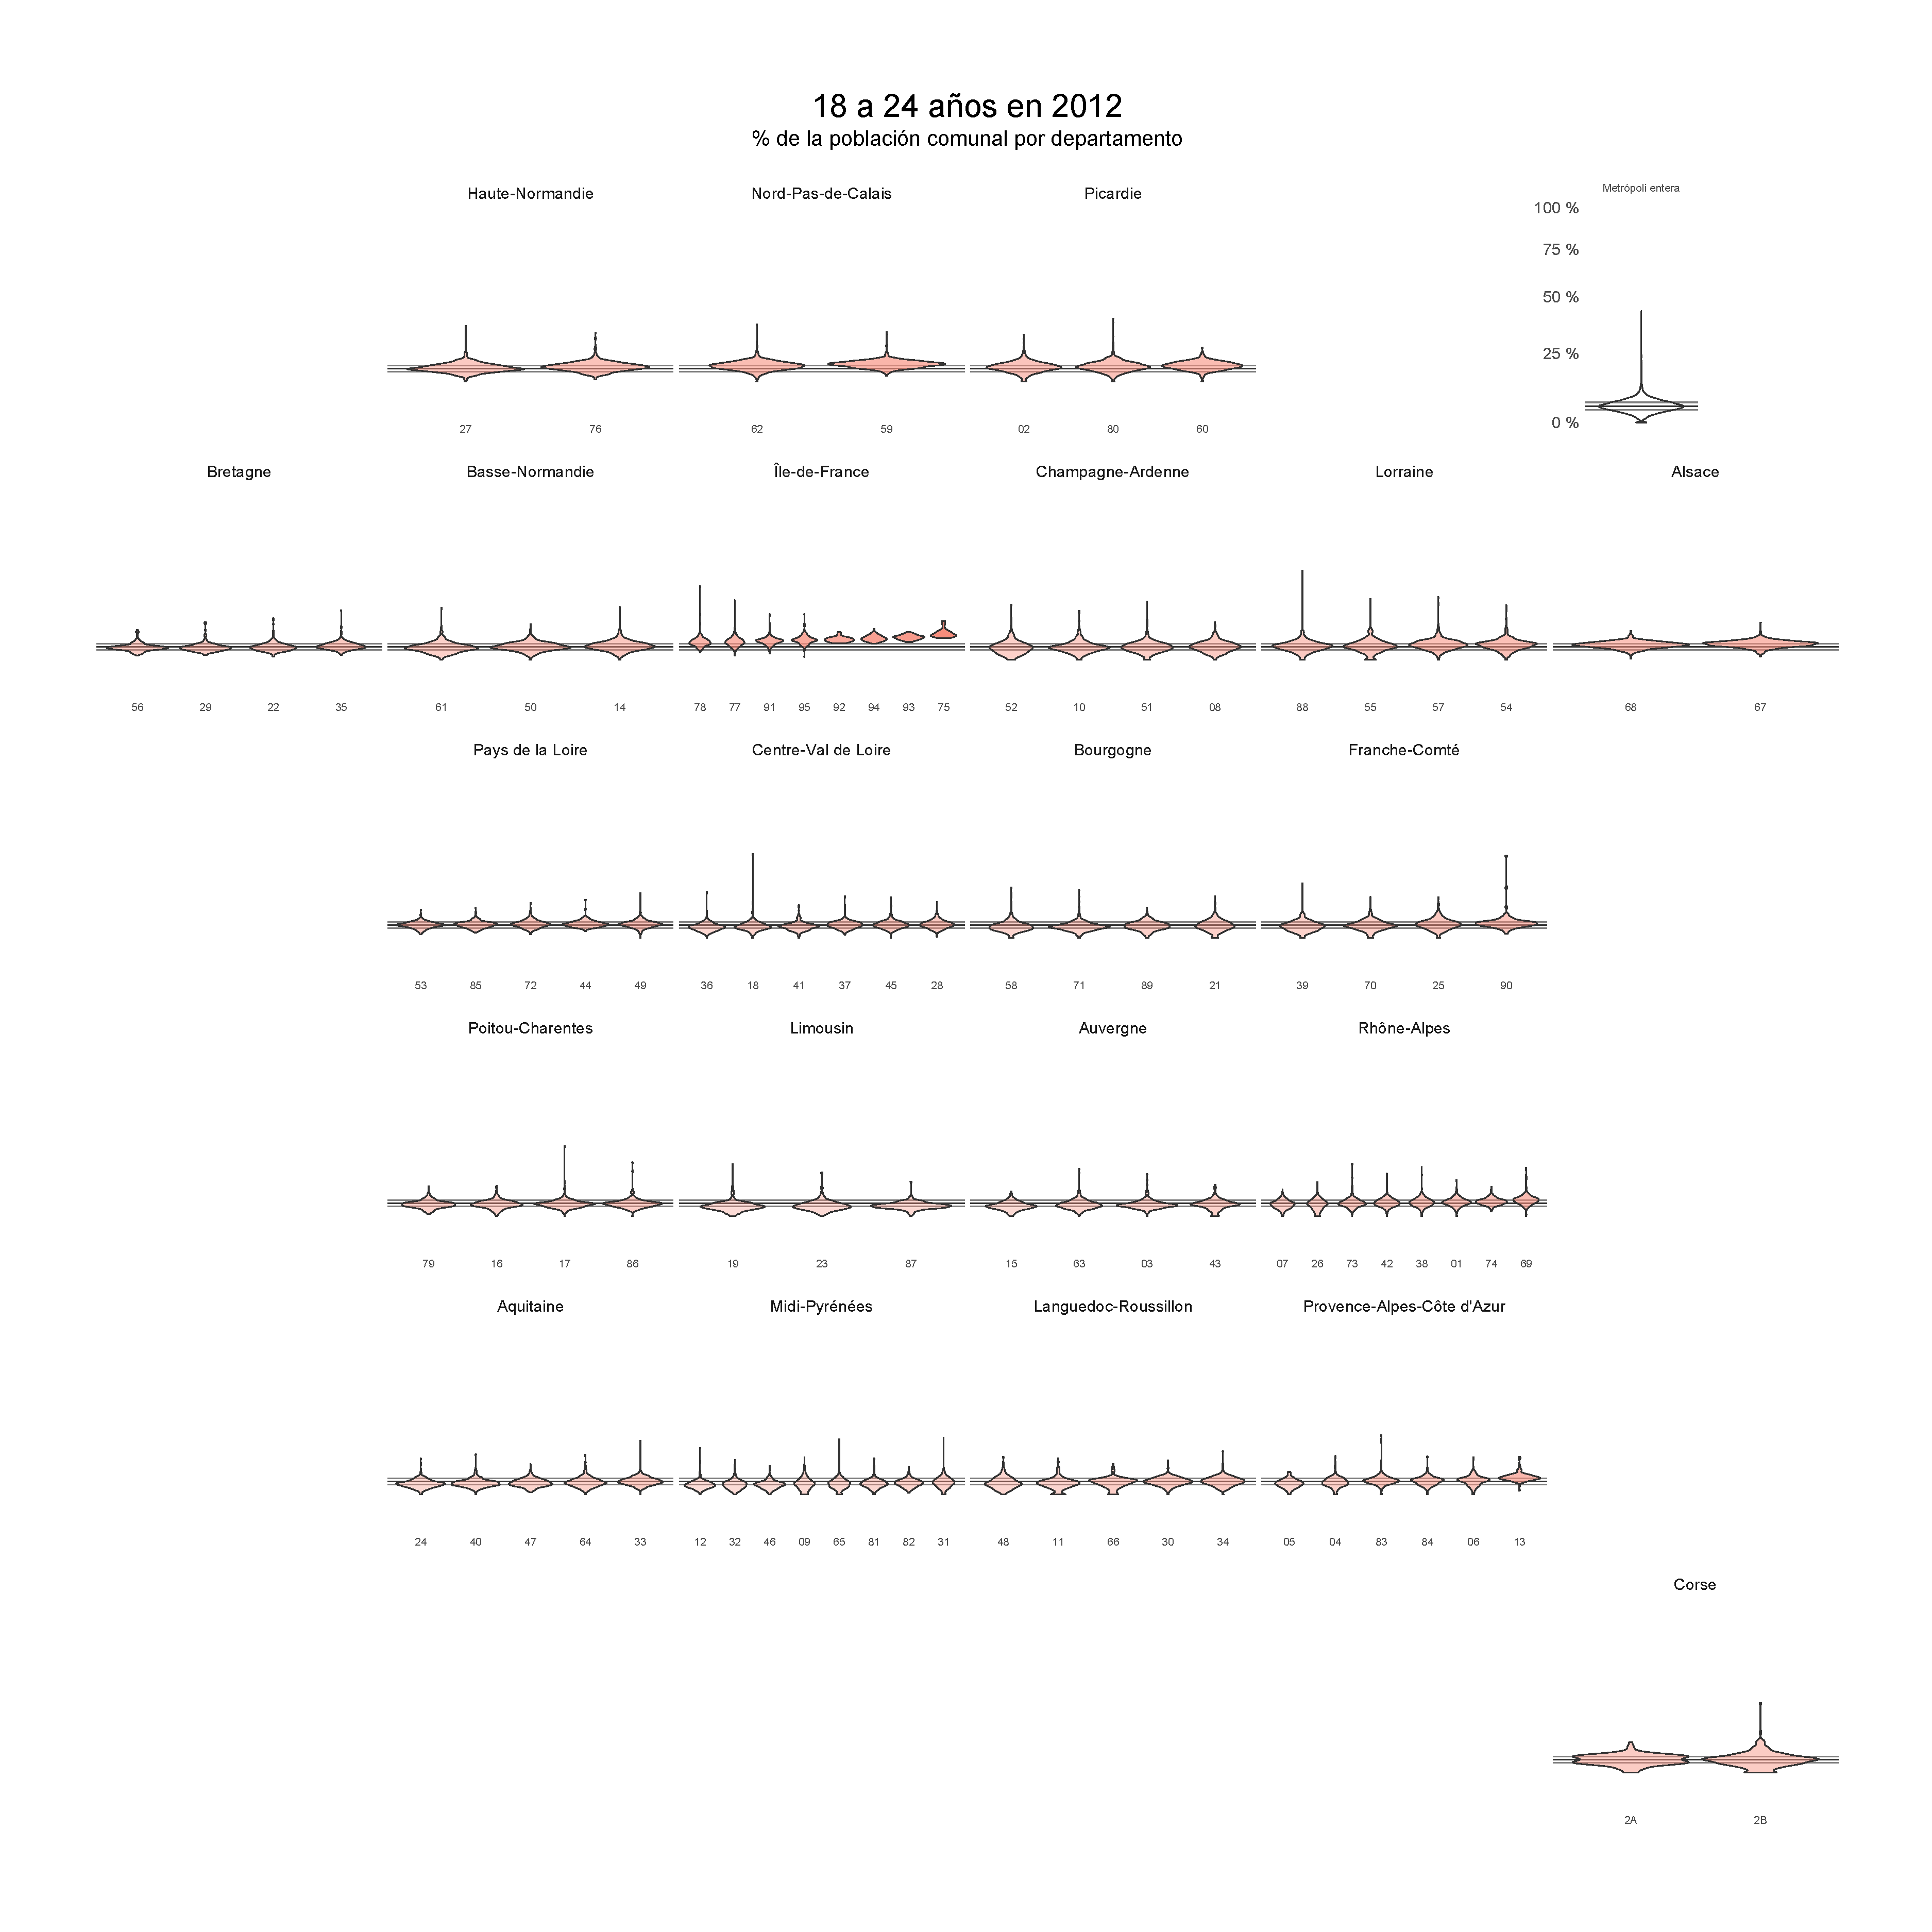
\includegraphics[width = \textwidth]{Figs/AED/Geofacet_Distr_por_Dpto_Ed2_2012}
	\end{subfigure}
	~
	\begin{subfigure}{0.3\textwidth}
	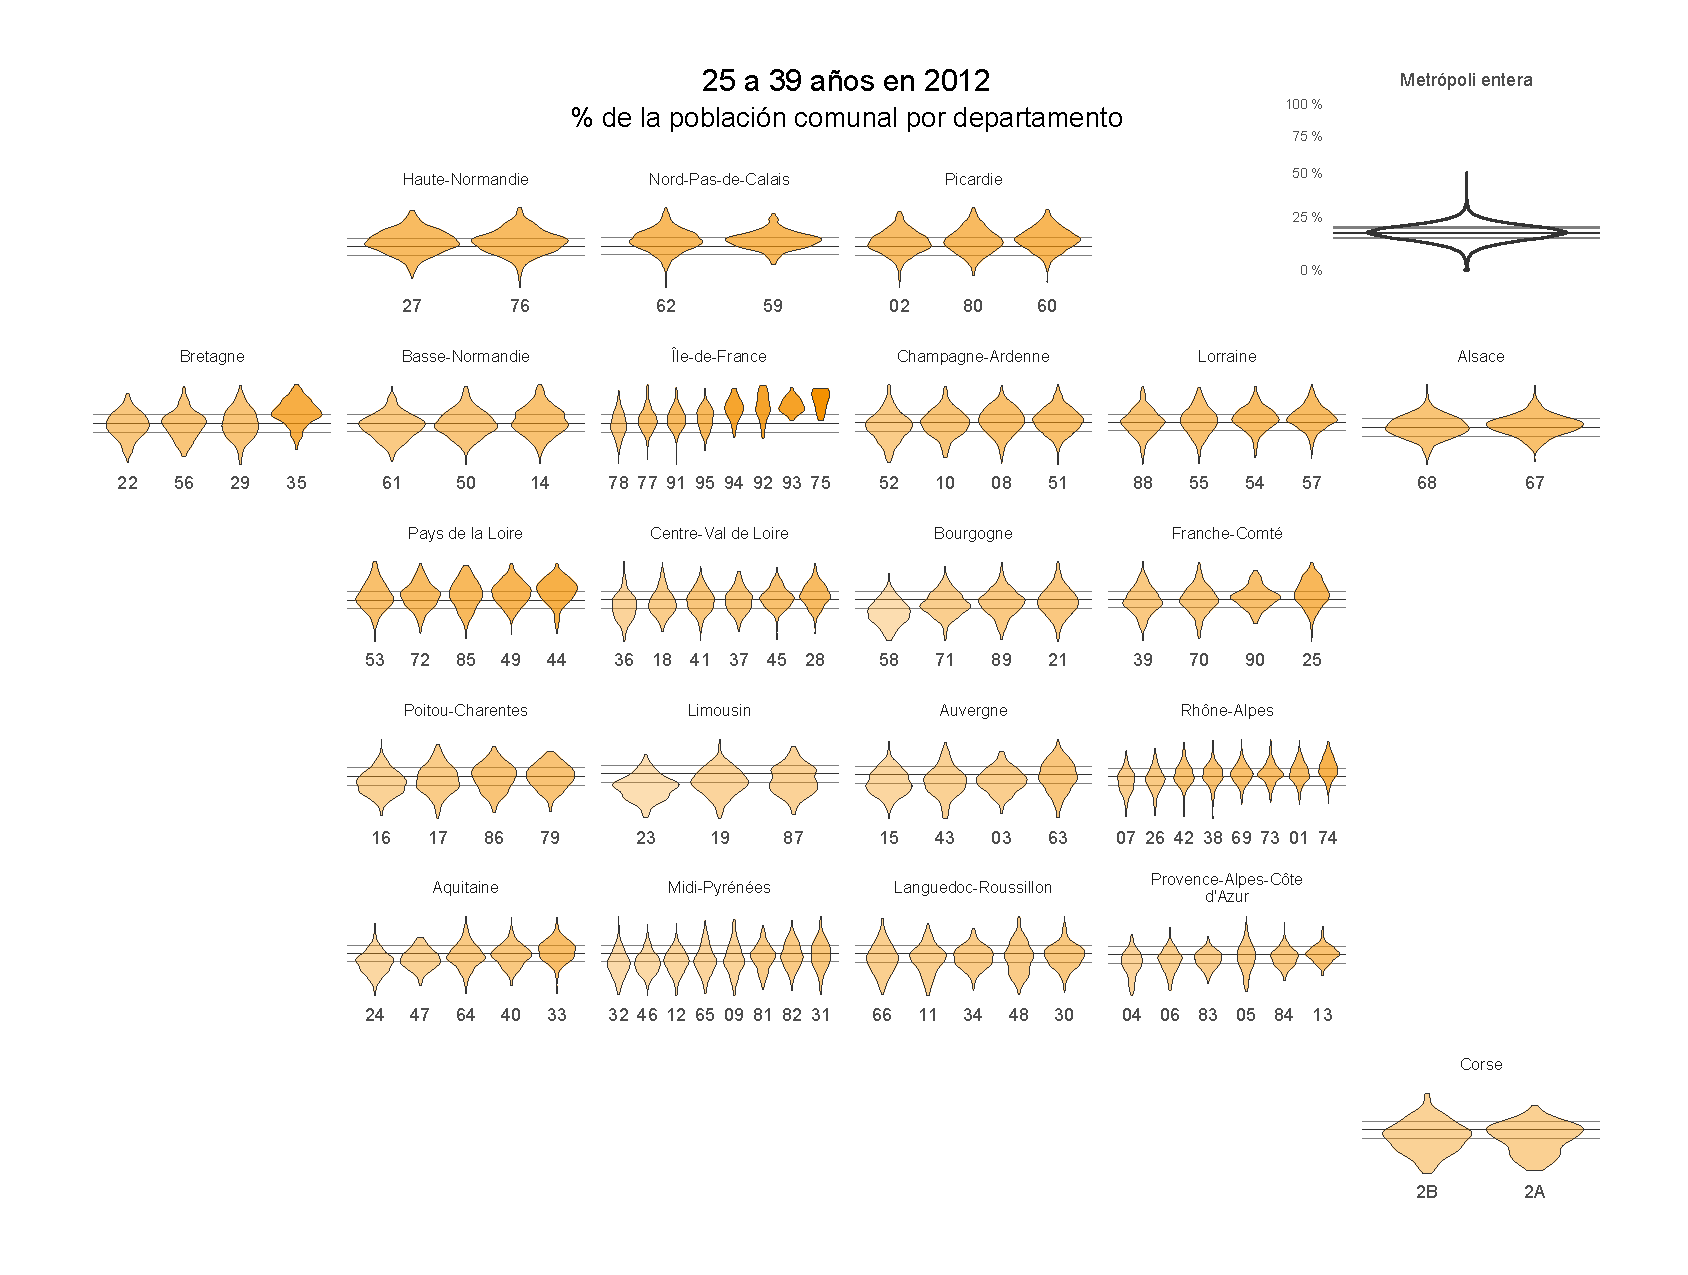
\includegraphics[width = \textwidth]{Figs/AED/Geofacet_Distr_por_Dpto_Ed3_2012}
	\end{subfigure}
	~
	\begin{subfigure}{0.3\textwidth}
	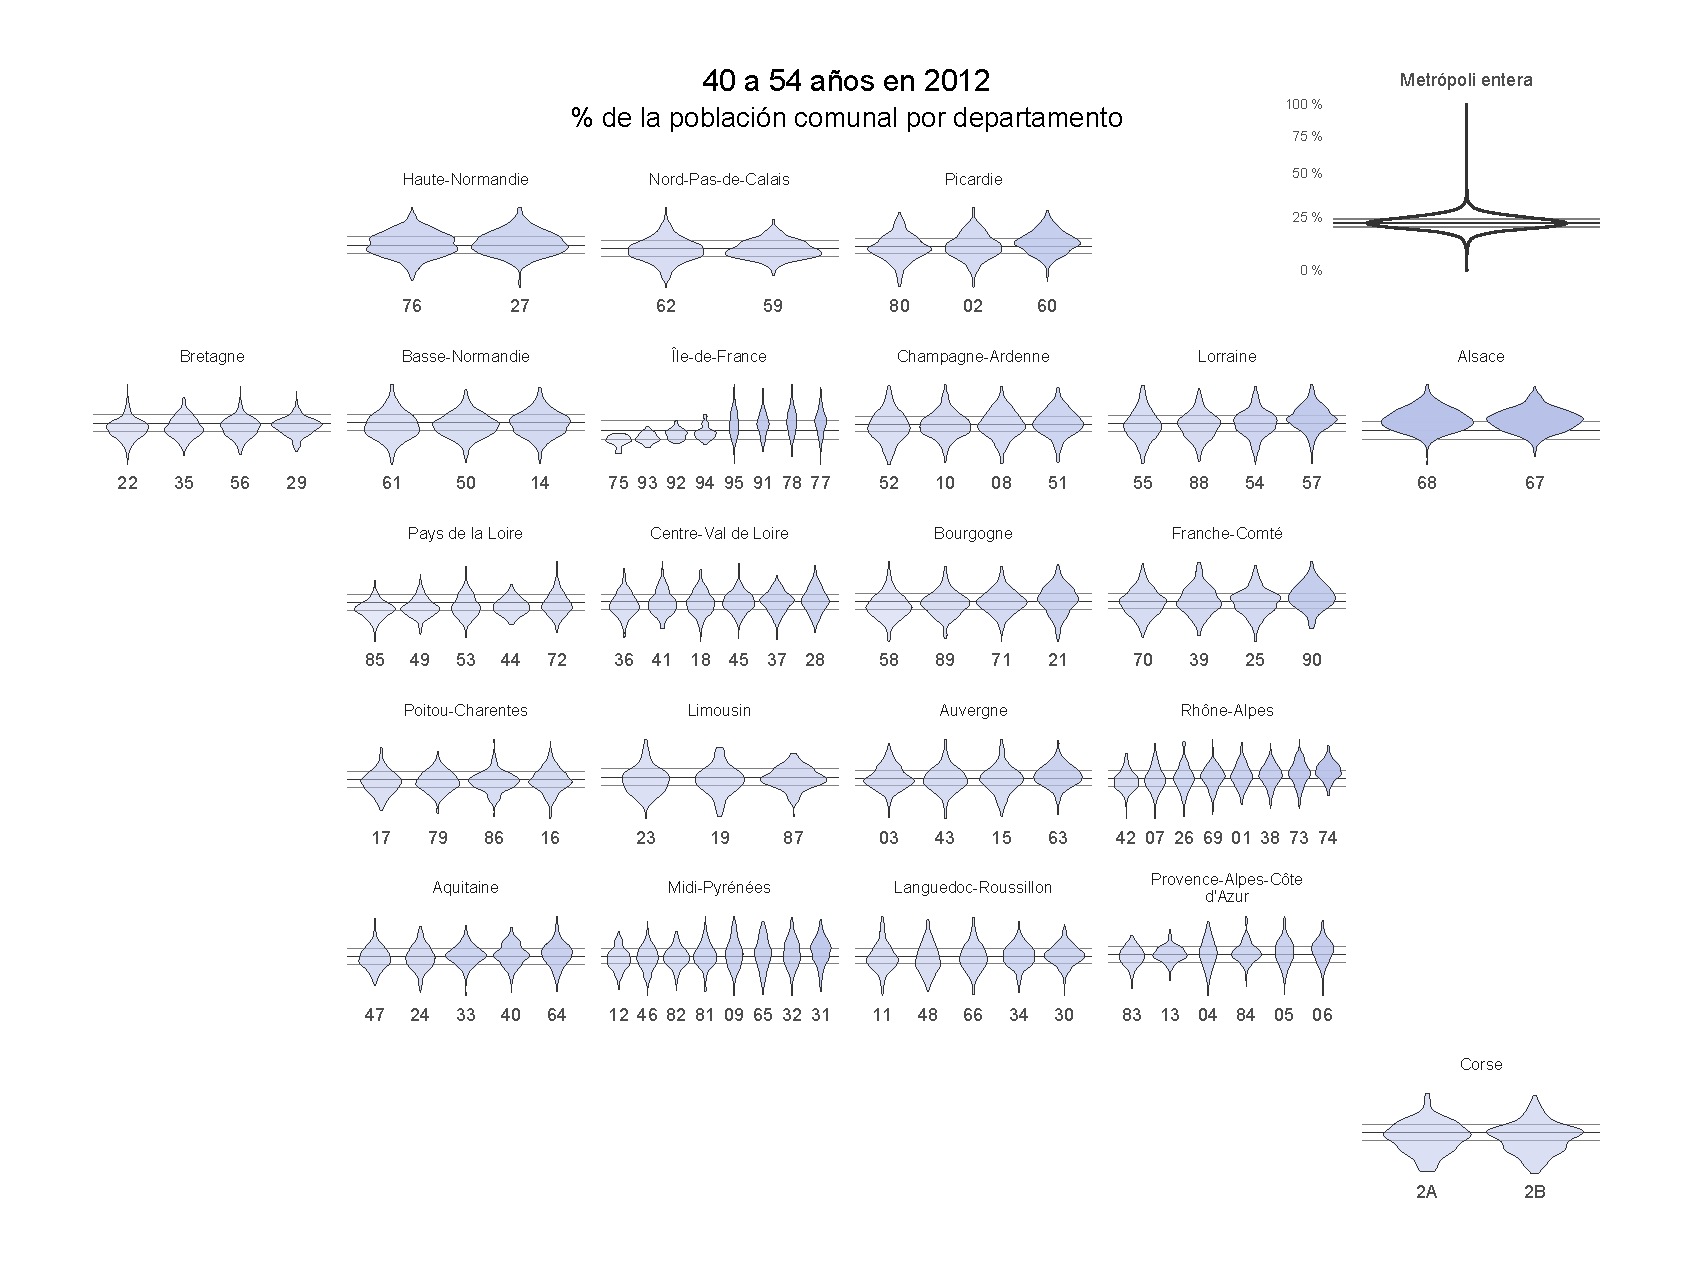
\includegraphics[width = \textwidth]{Figs/AED/Geofacet_Distr_por_Dpto_Ed4_2012}
	\end{subfigure}
	~
	\begin{subfigure}{0.3\textwidth}
	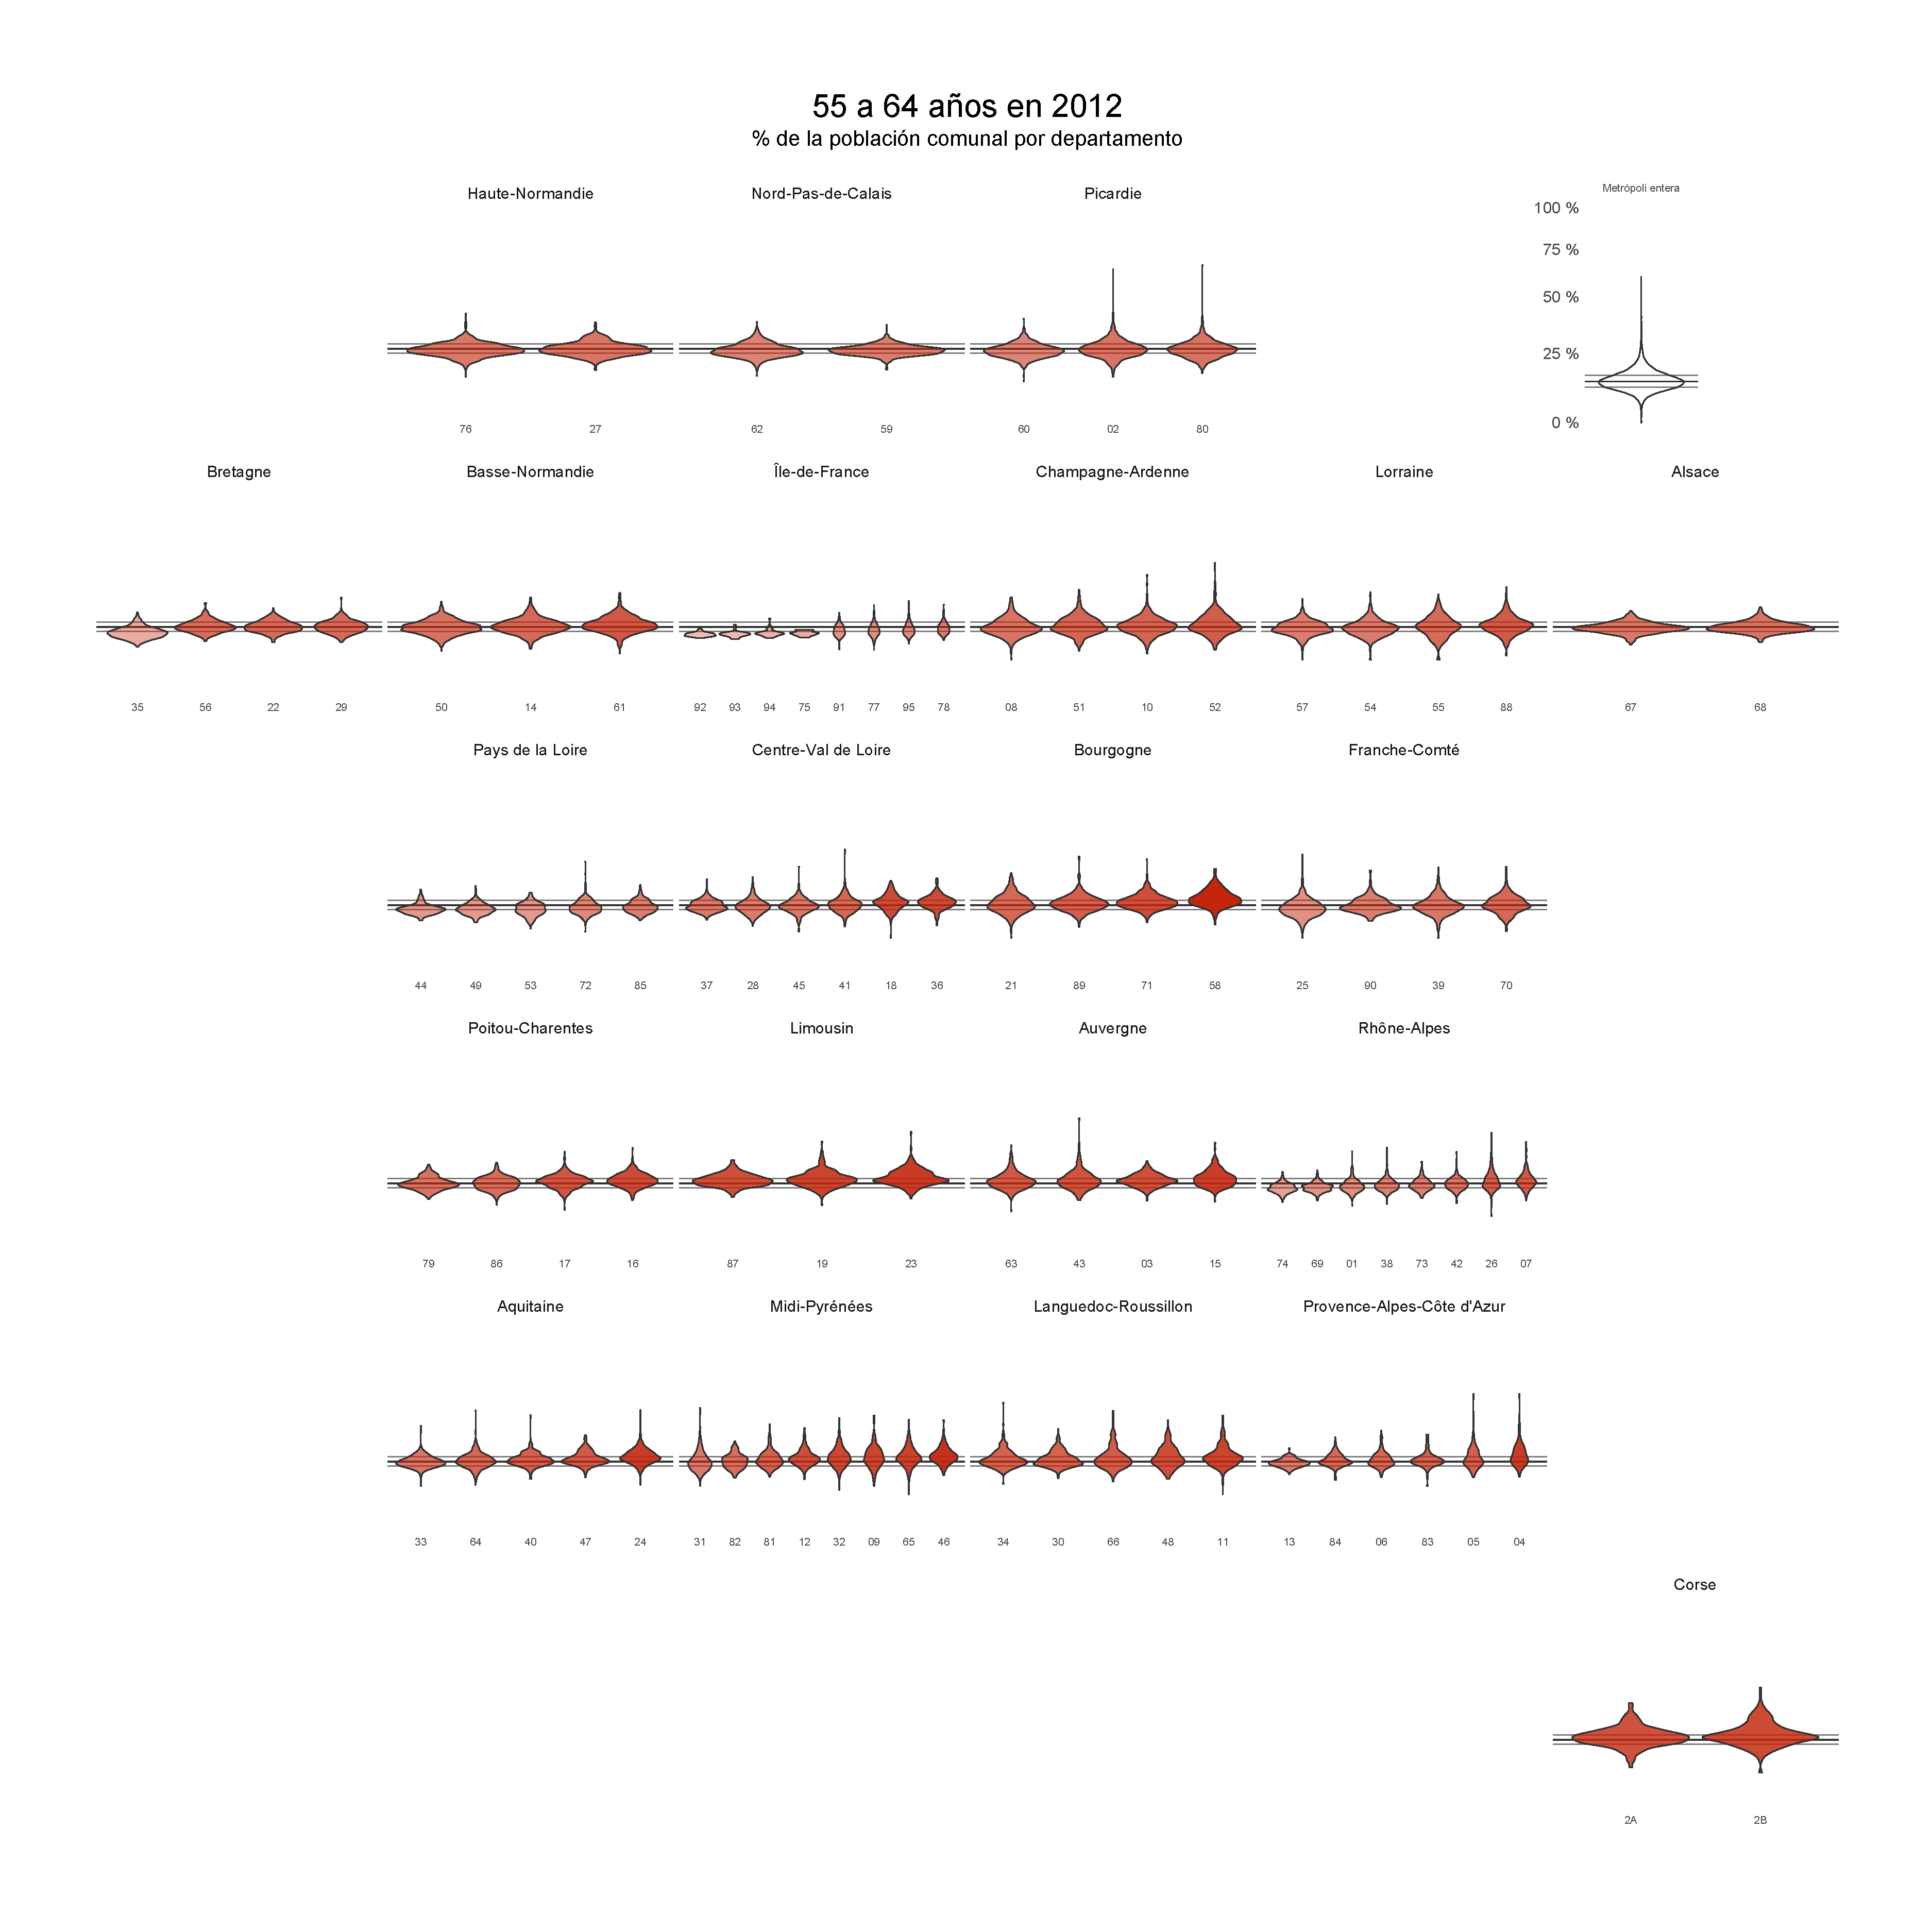
\includegraphics[width = \textwidth]{Figs/AED/Geofacet_Distr_por_Dpto_Ed5_2012}
	\end{subfigure}
	~
	\begin{subfigure}{0.3\textwidth}
	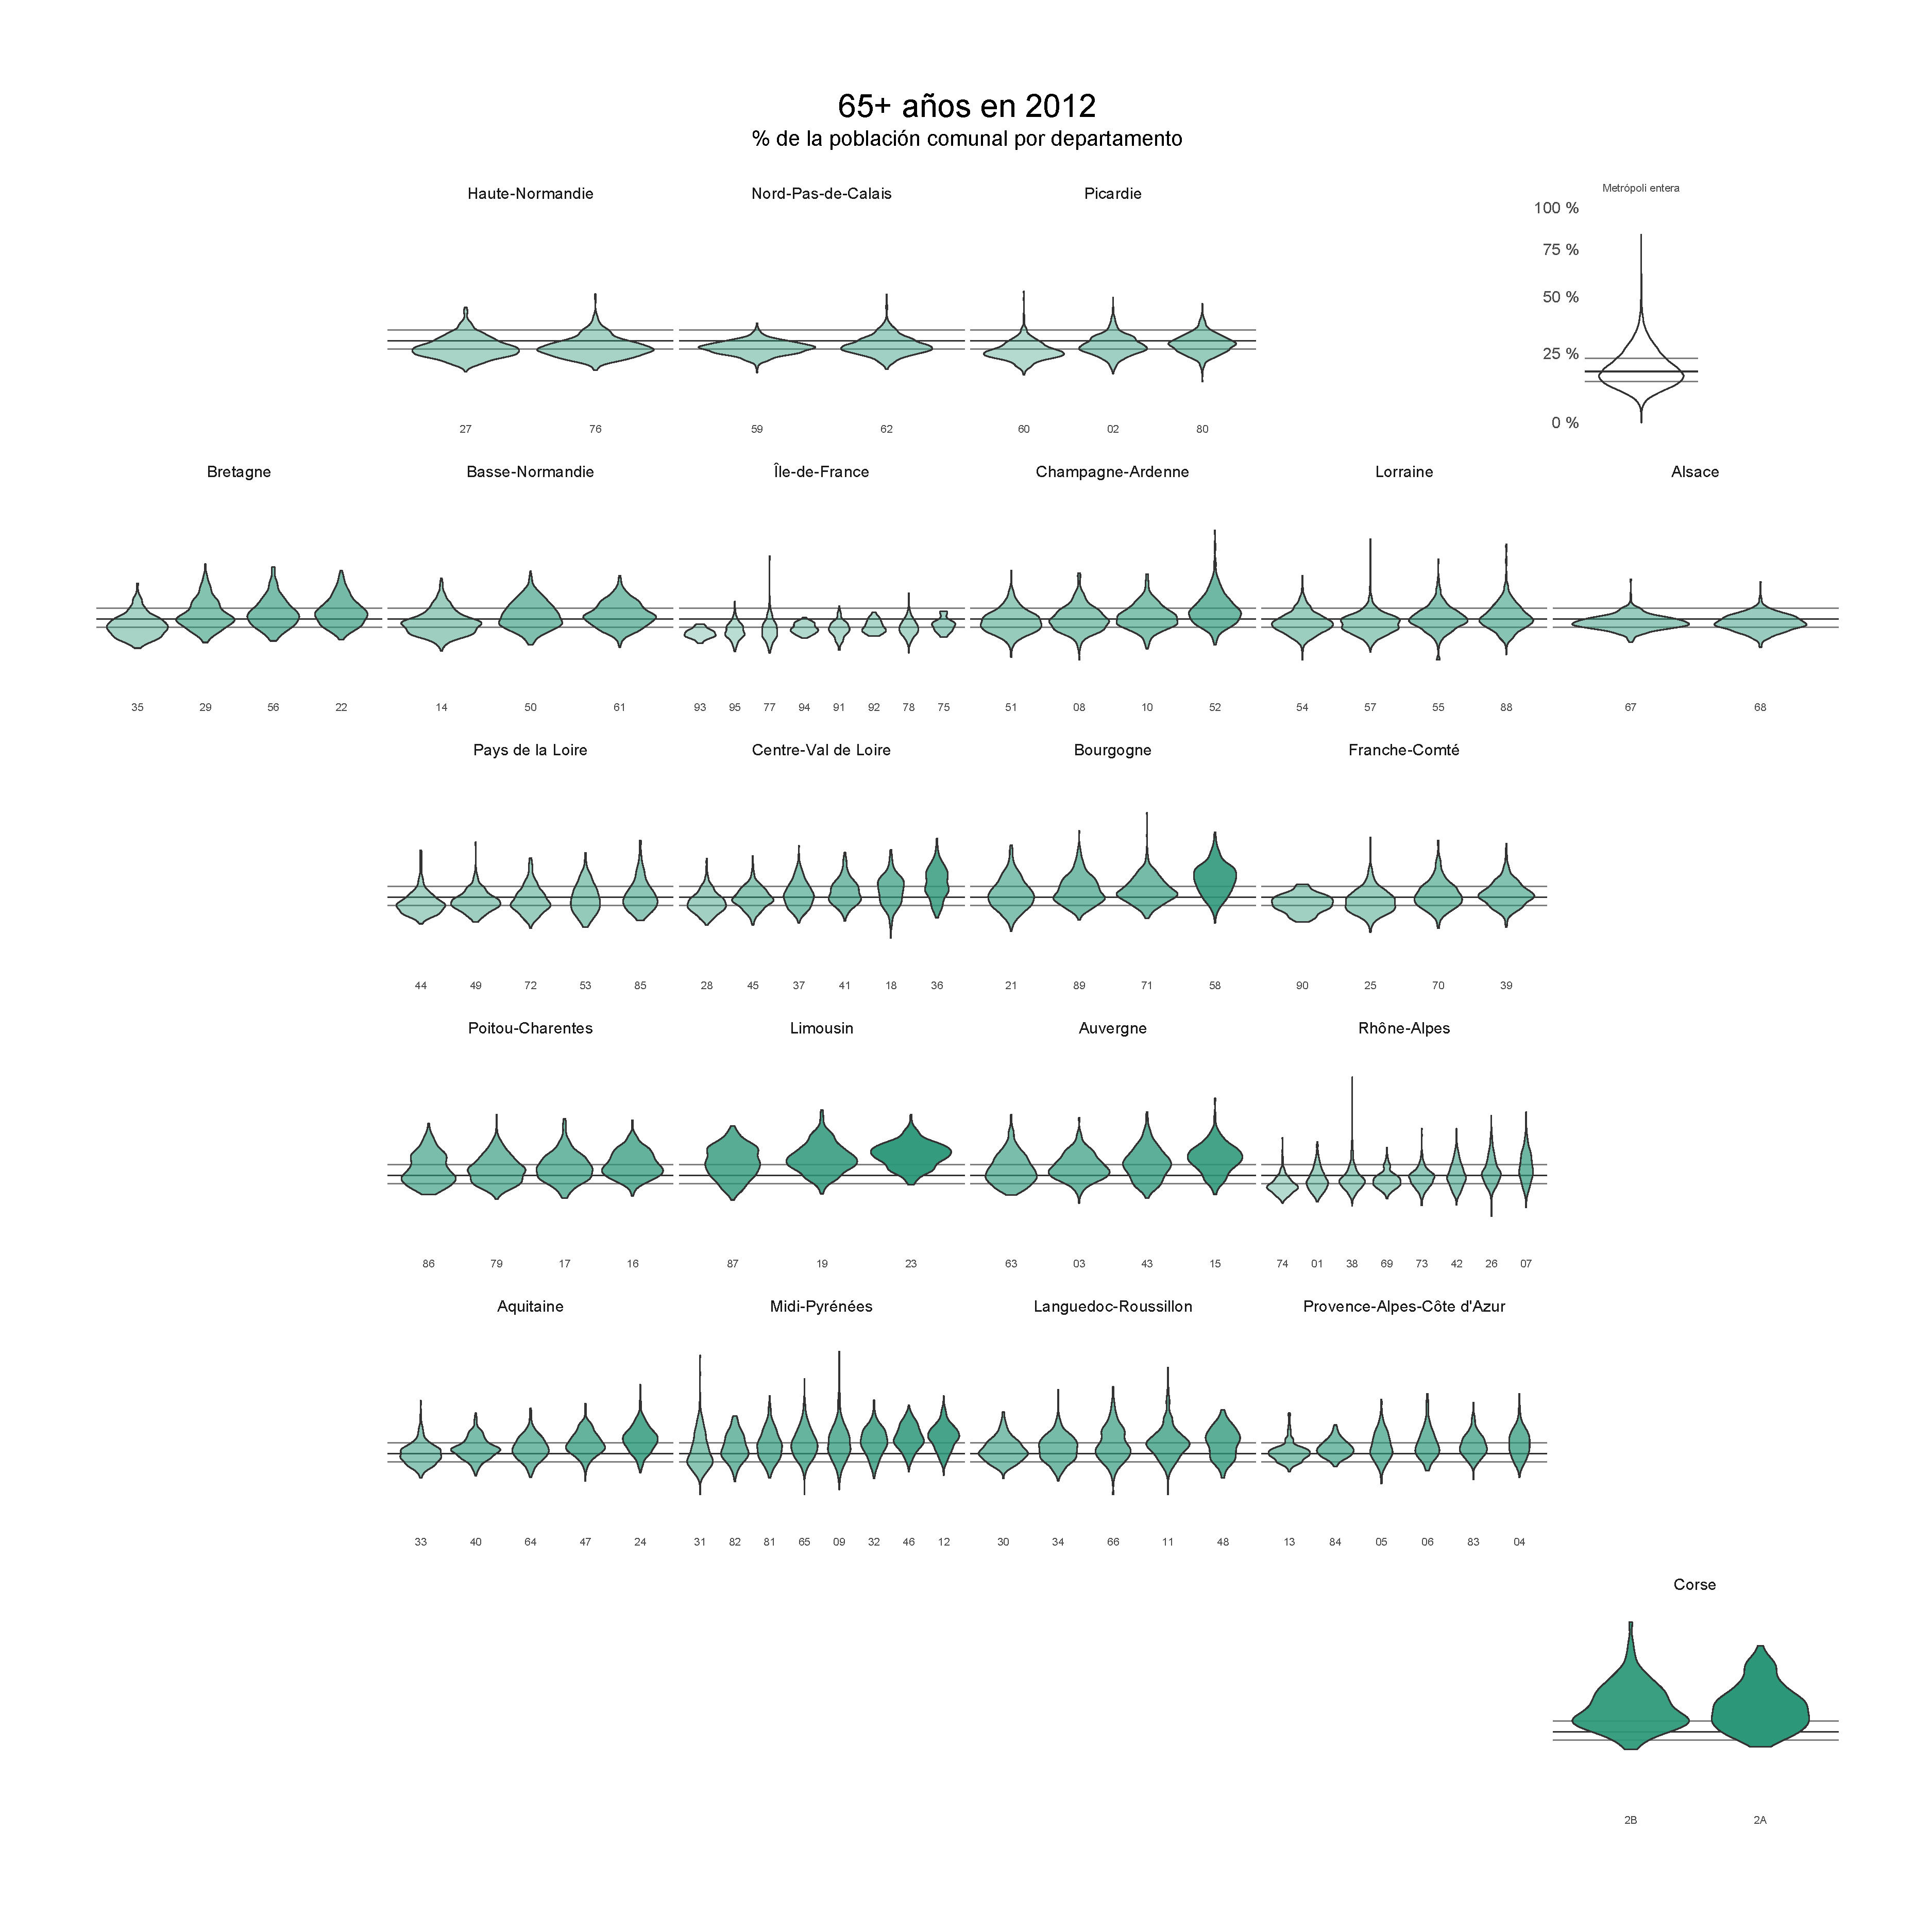
\includegraphics[width = \textwidth]{Figs/AED/Geofacet_Distr_por_Dpto_Ed6_2012}
	\end{subfigure}
	\caption{Distribuciones departamentales del porcentaje de los distintos grupos de edad como proporción de la población de las comunas en 2012. Fuente: elaboración propia con los datos censales.}
	\label{fig:Distr_por_Dpto_Edades_2012}	
\end{figure}

Finalmente, vemos en la \textbf{Figura \ref{fig:Distr_por_Dpto_CSP_2012}} las distribuciones para las diferentes categorías socioprofesionales. El primer dato que salta a la vista es que la región parisina tiene una composición socioprofesional muy particular. En efecto, Île de France es una región que comparativamente hablando, casi no tiene agricultores, obreros o retirados. Por el contrario, tiene un fuerte componente de los llamados cuadros y profesiones intelectuales superiores, pero su distribución es distinta a través de los departamentos que conforman la zona metropolitana. Dentro de la ciudad de París--- departamento 75--- representan el mayor porcentaje. Pero también forman un porcentaje importante de las poblaciones comunales de los departamentos al poniente y al sur de este departamento.  Estos departamentos son el 92-Hauts-de-Seine y 94-Val-de-Marne, dentro de la llamada \textit{pequeña corona} de París y los departamentos occidentales de la \textit{gran corona} de París, que incluye 78-Yvelines, 91-Essonne y 95-Val-d'Oise. Por el contrario, en el oriente de la zona metropolitana, en los departamentos de 93-Seine-Saint-Denis y 77-Seine-et-Marne, viven los empleados de la urbe. Las profesiones intermediarias viven más bien en la \textit{gran corona}, es decir en los departamentos 77, 78, 91 y 95.\\
 
\begin{sidewaysfigure}[h]
	\centering
	\begin{subfigure}{0.235\textwidth}
	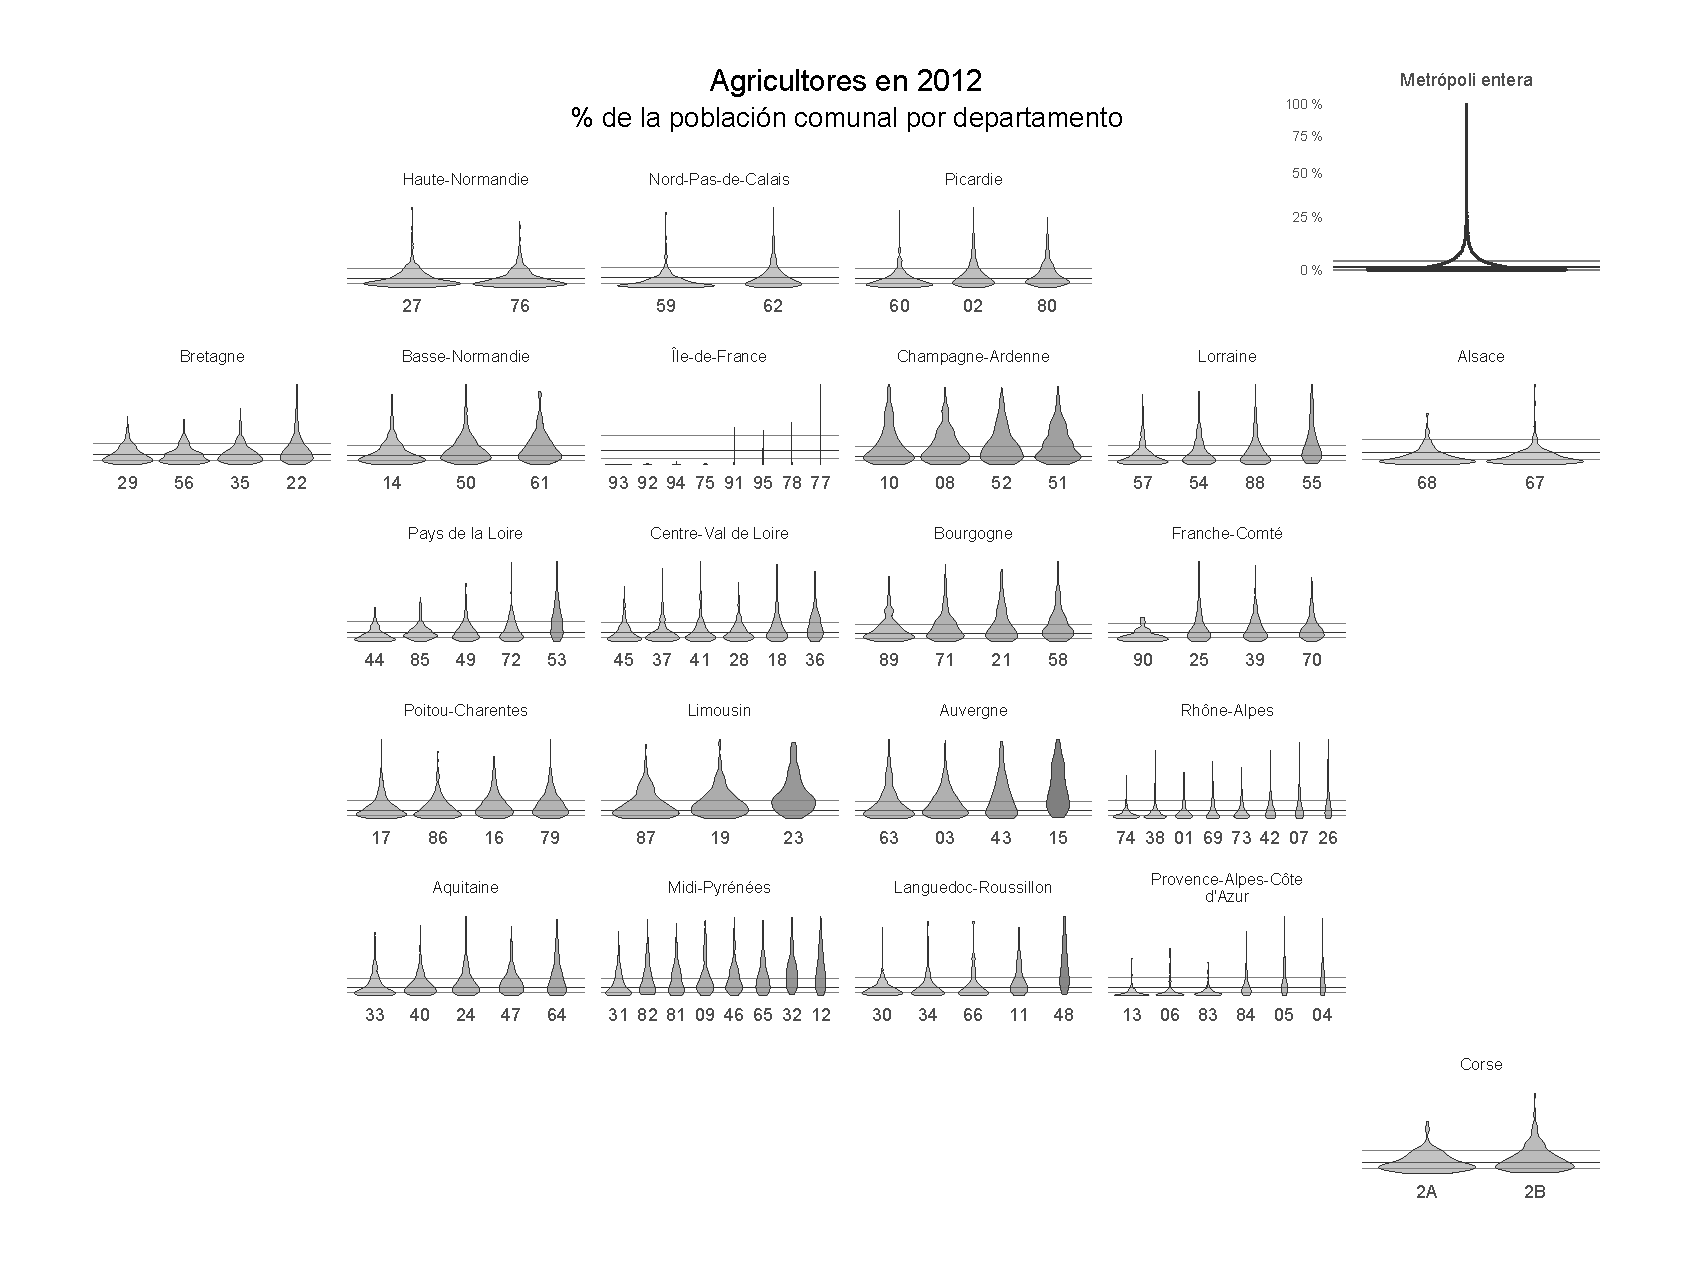
\includegraphics[width = \textwidth]{Figs/AED/Geofacet_Distr_por_Dpto_CSP1_2012}
	\end{subfigure}
	~
	\begin{subfigure}{0.235\textwidth}
	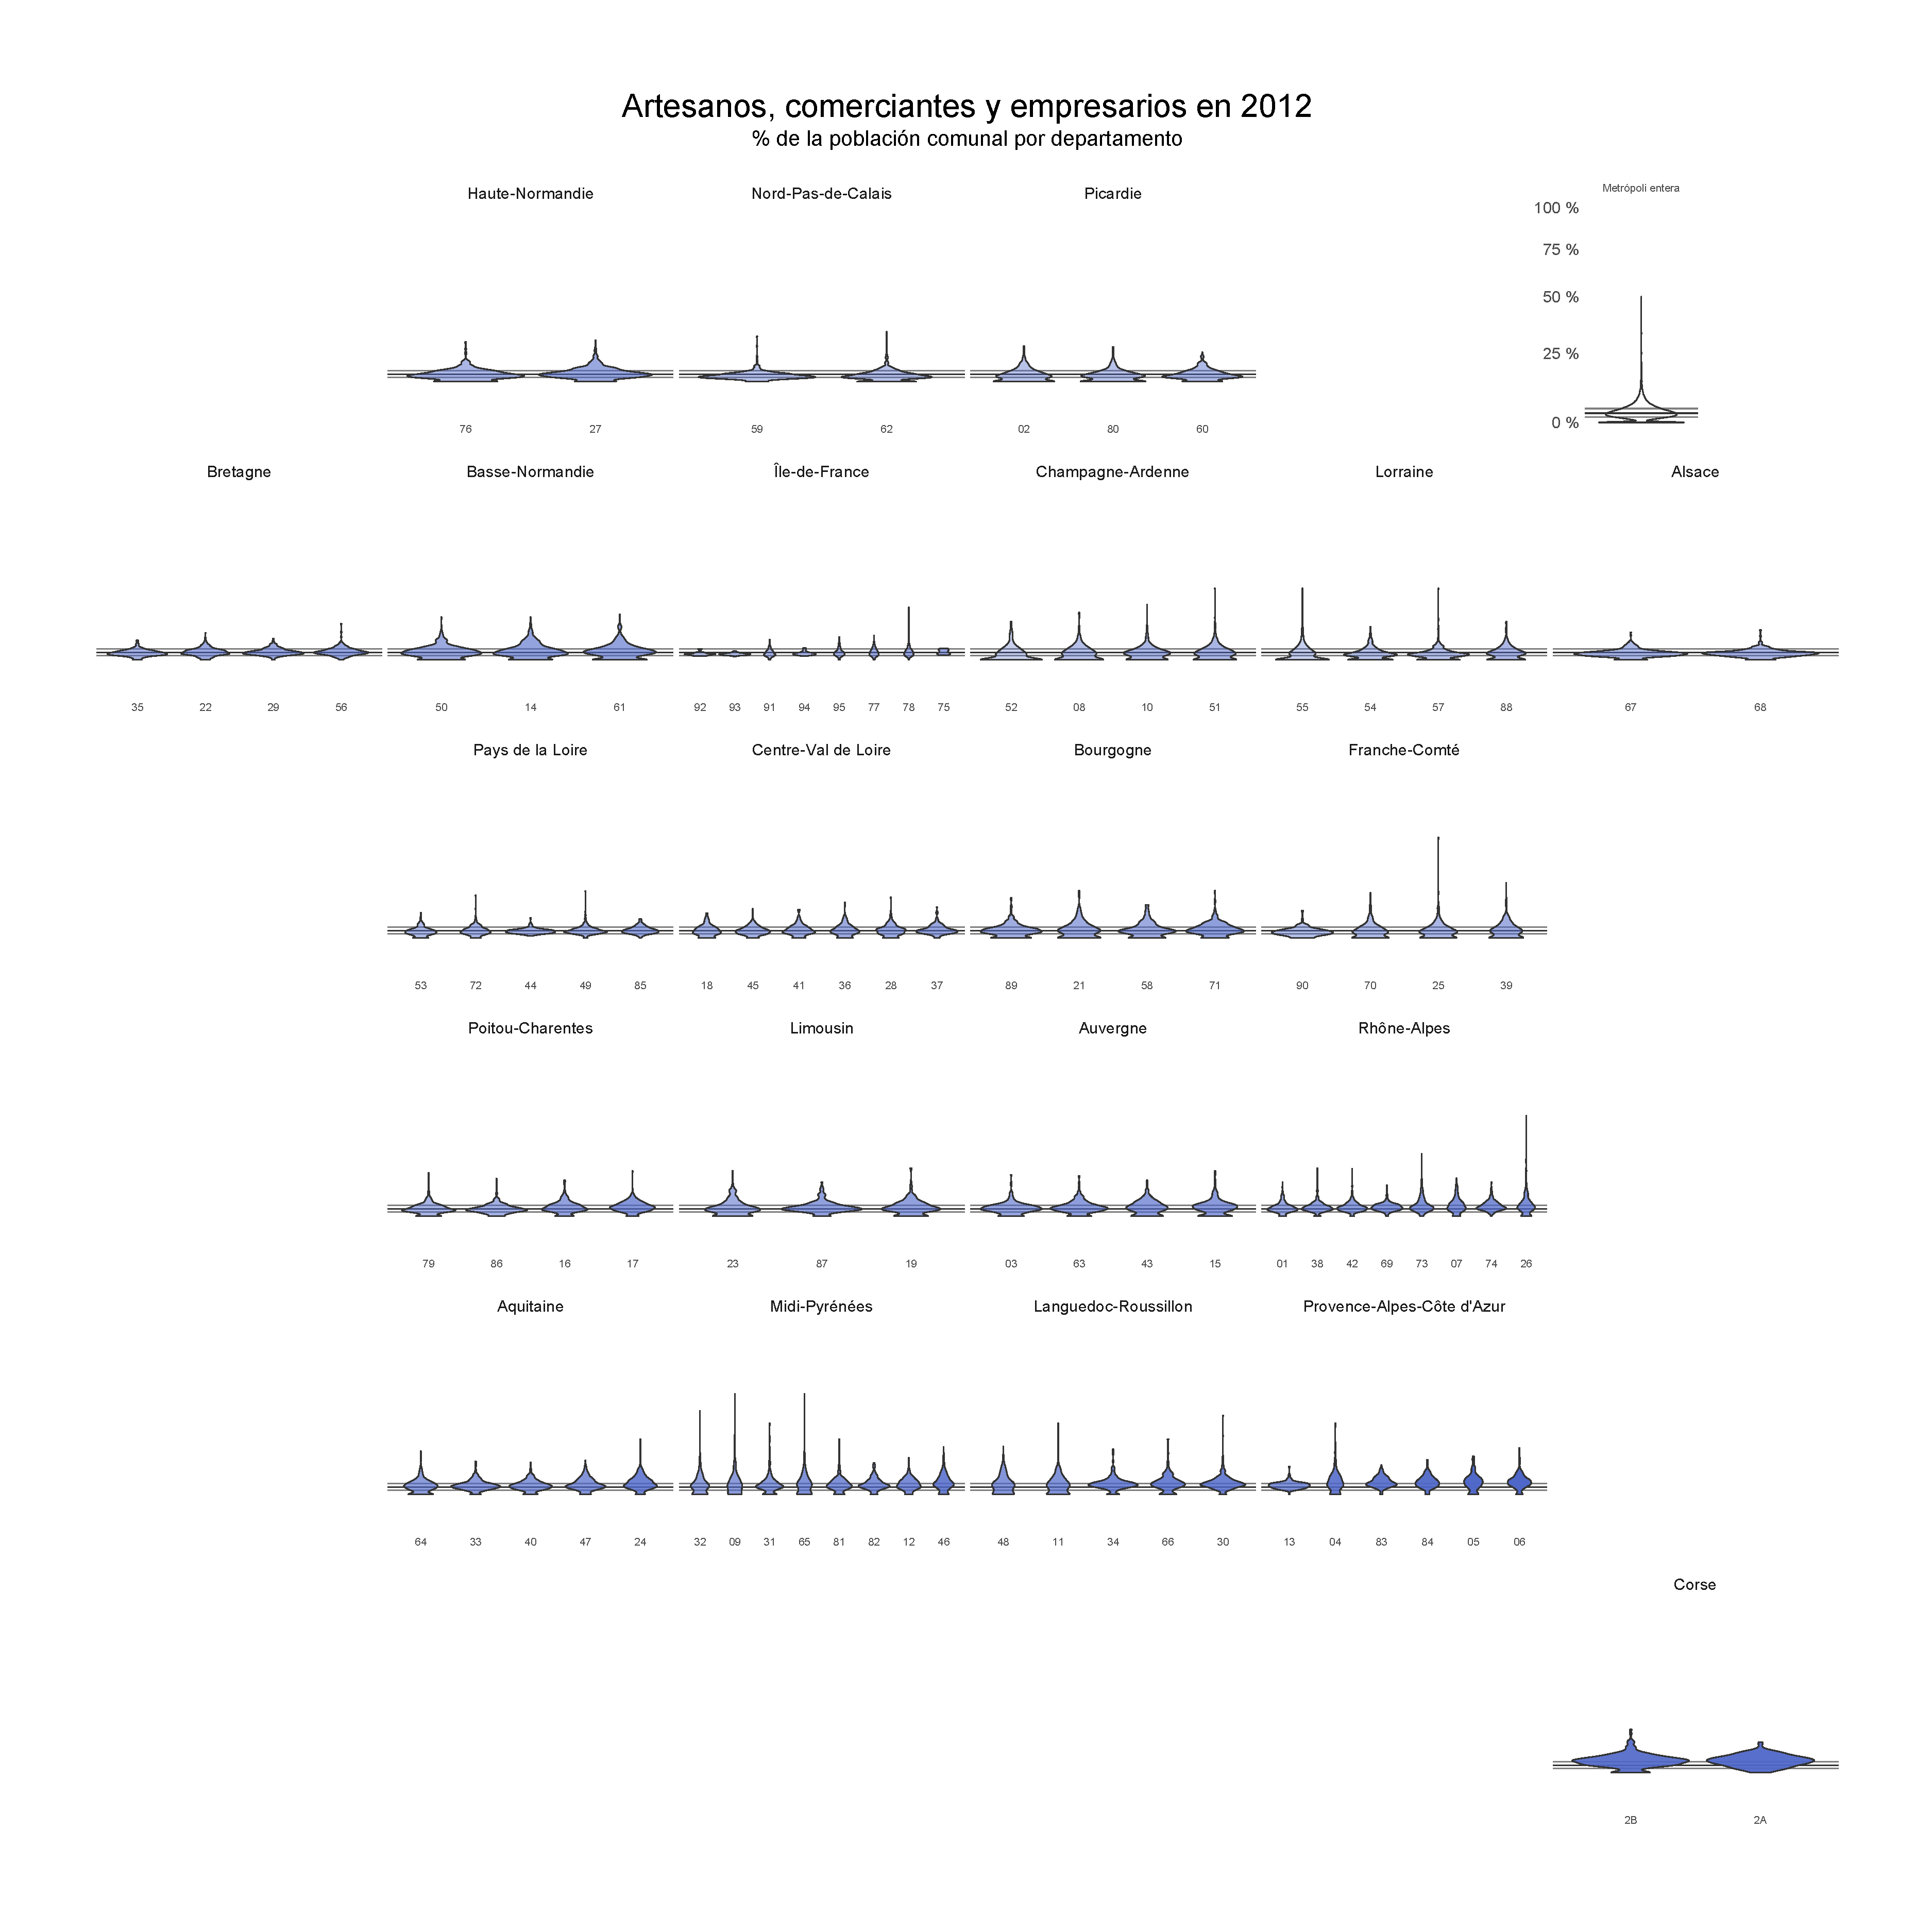
\includegraphics[width = \textwidth]{Figs/AED/Geofacet_Distr_por_Dpto_CSP2_2012}
	\end{subfigure}
	~
	\begin{subfigure}{0.235\textwidth}
	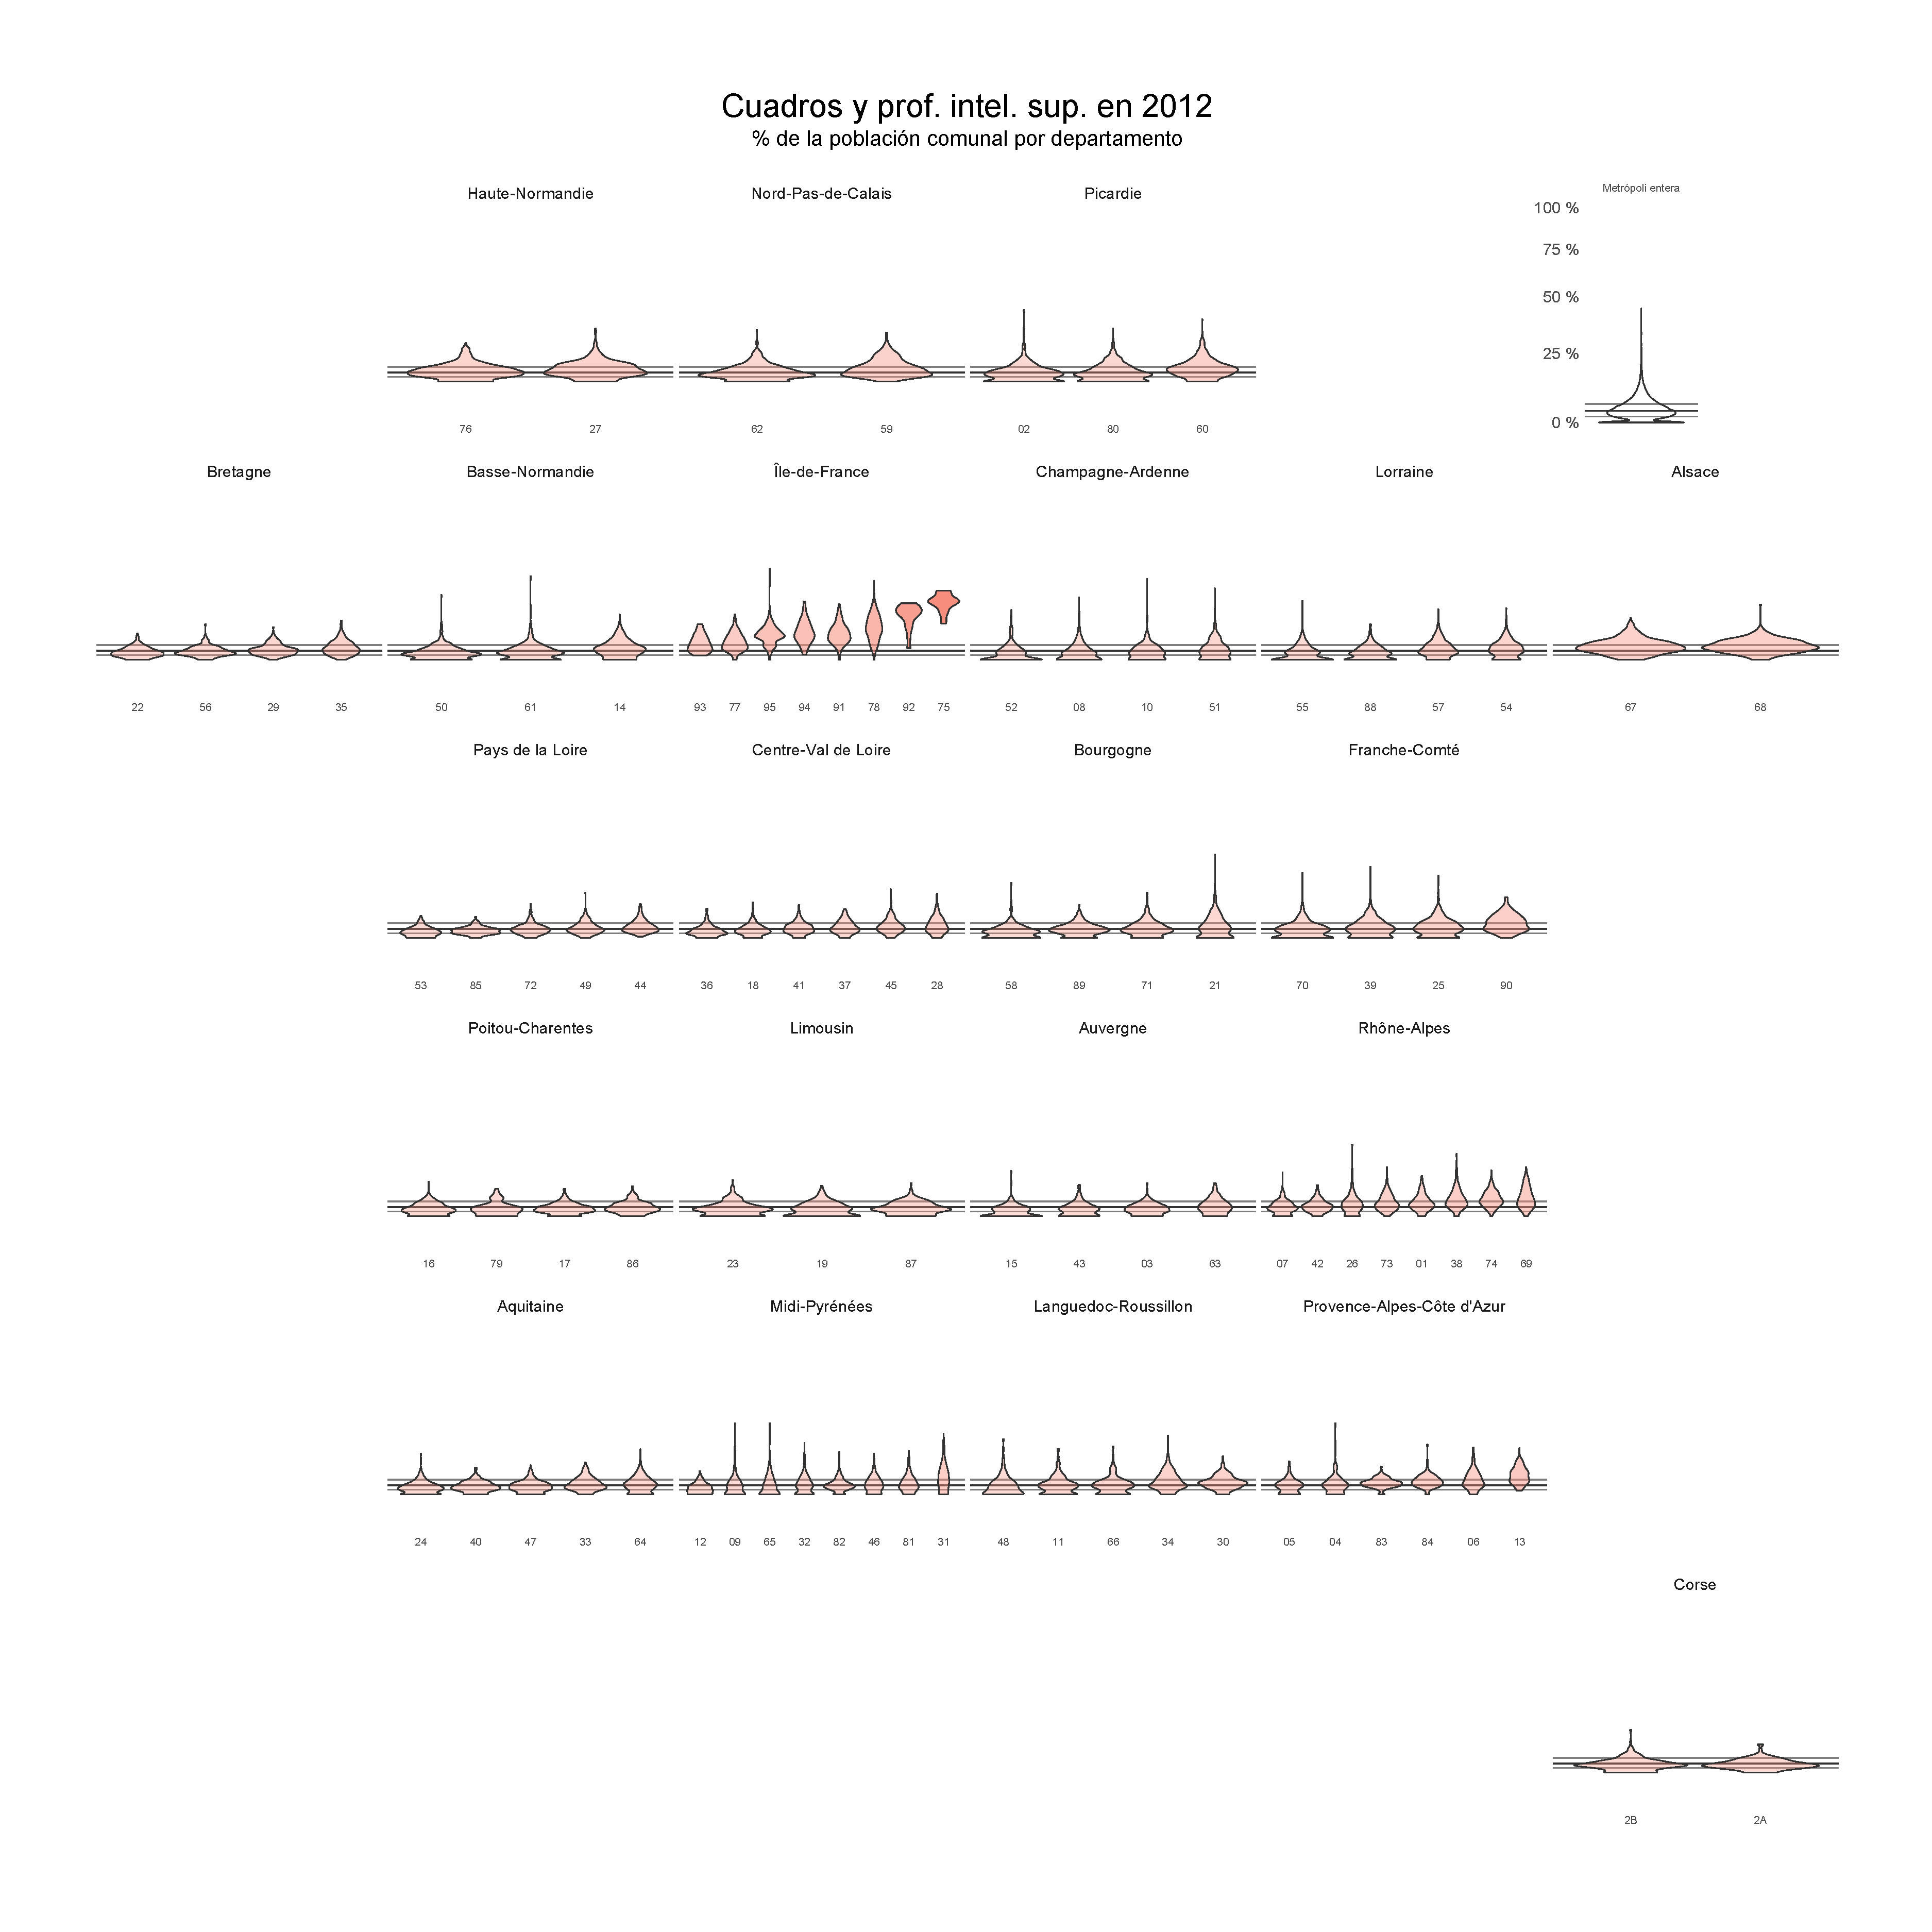
\includegraphics[width = \textwidth]{Figs/AED/Geofacet_Distr_por_Dpto_CSP3_2012}
	\end{subfigure}
	~
	\begin{subfigure}{0.235\textwidth}
	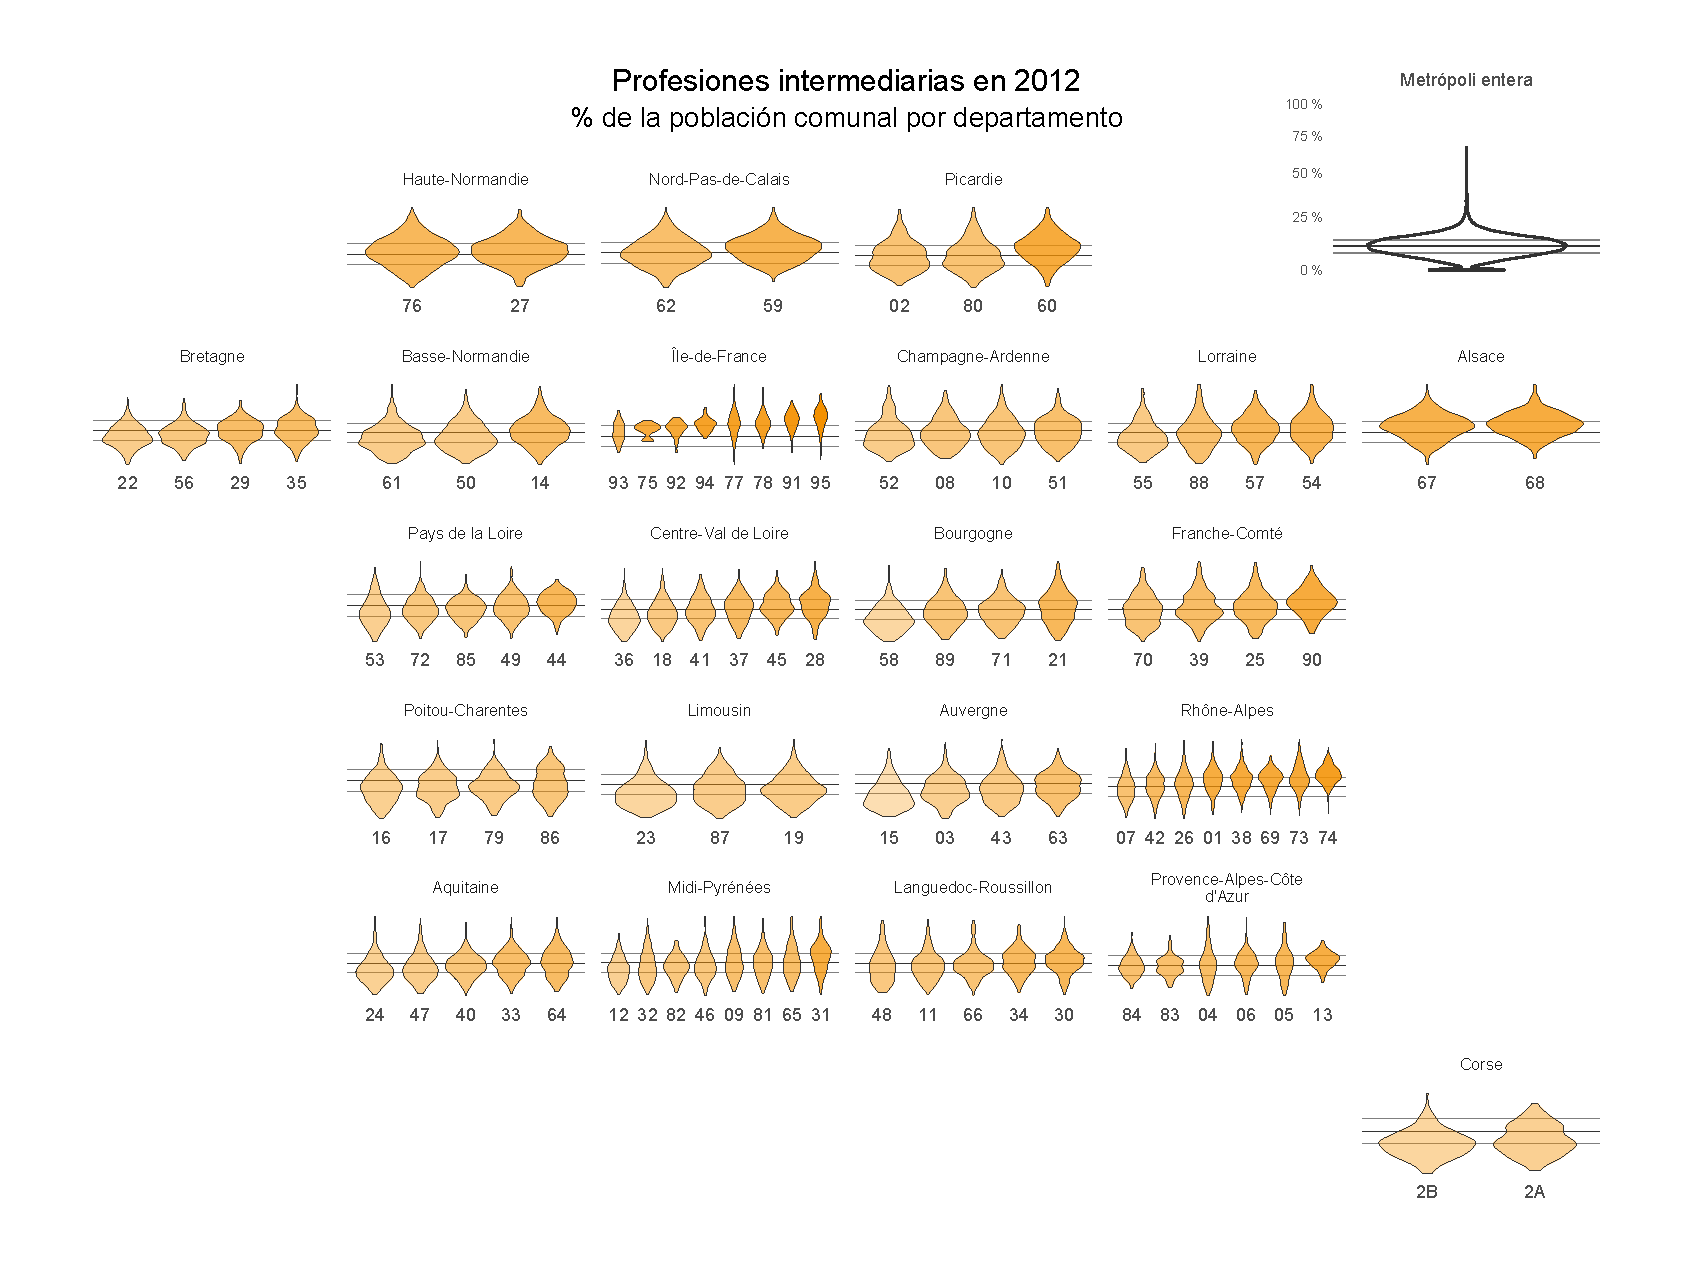
\includegraphics[width = \textwidth]{Figs/AED/Geofacet_Distr_por_Dpto_CSP4_2012}
	\end{subfigure}
	~
	\begin{subfigure}{0.235\textwidth}
	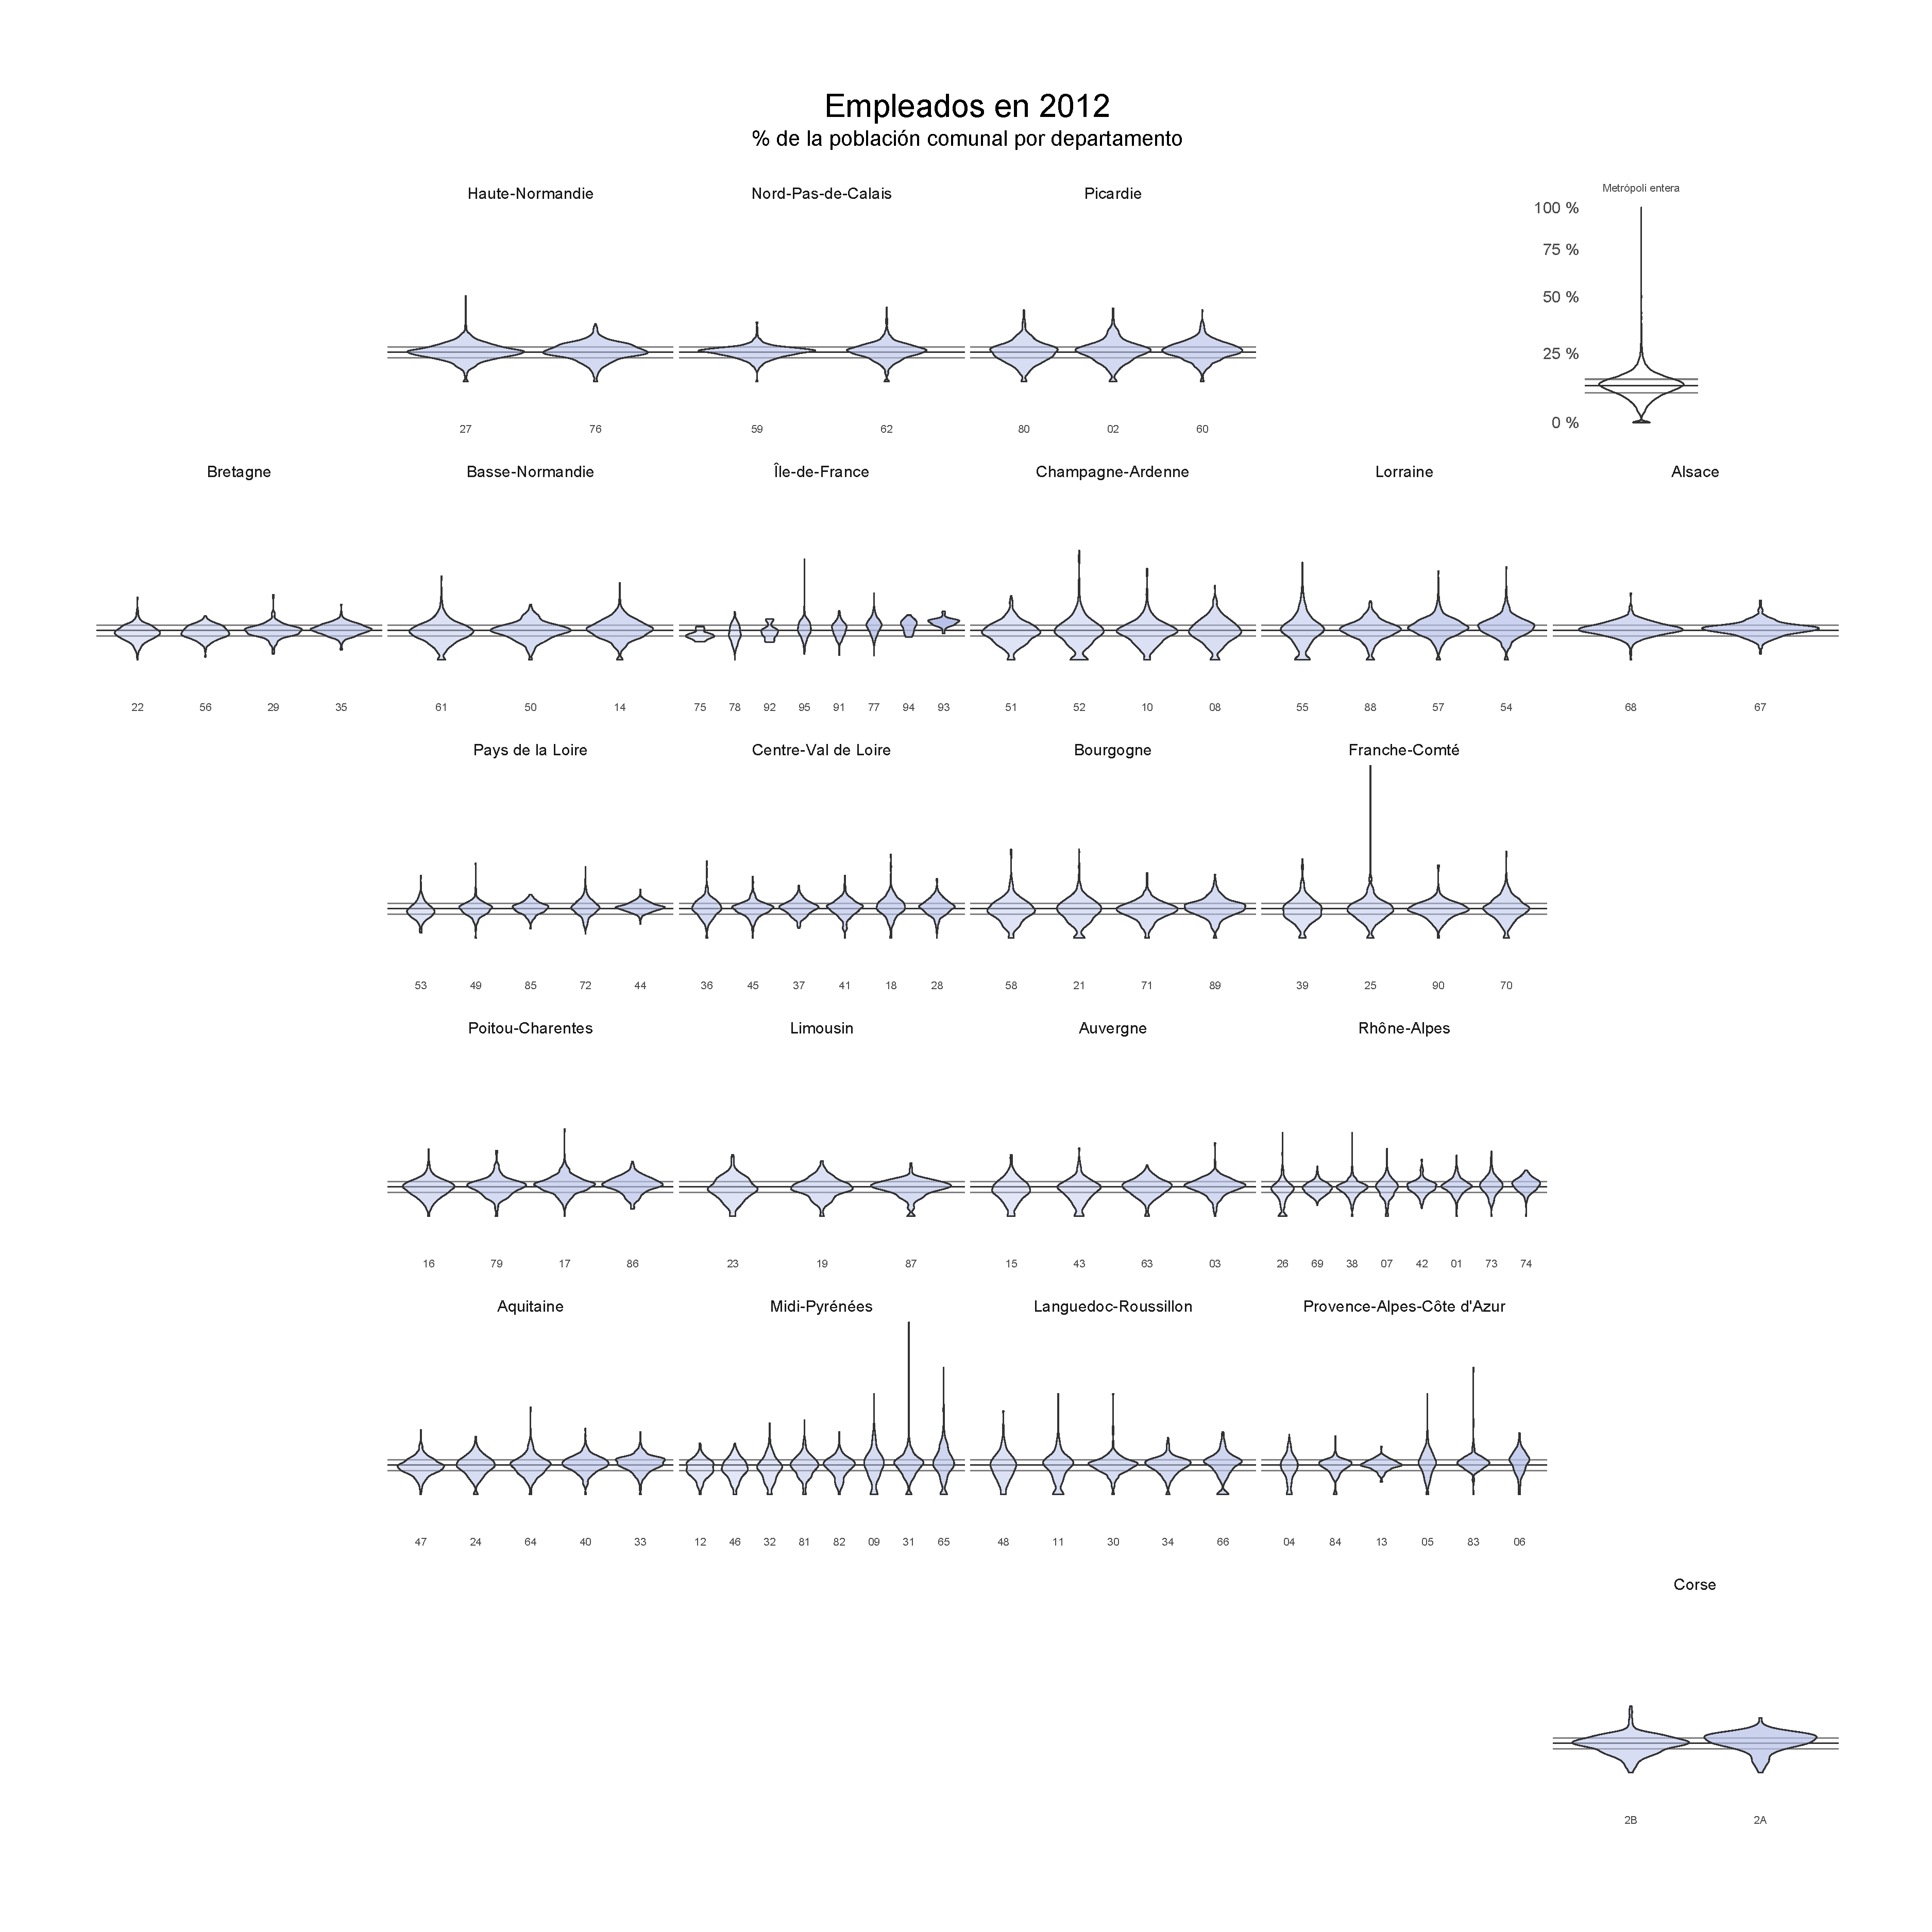
\includegraphics[width = \textwidth]{Figs/AED/Geofacet_Distr_por_Dpto_CSP5_2012}
	\end{subfigure}
	~
	\begin{subfigure}{0.235\textwidth}
	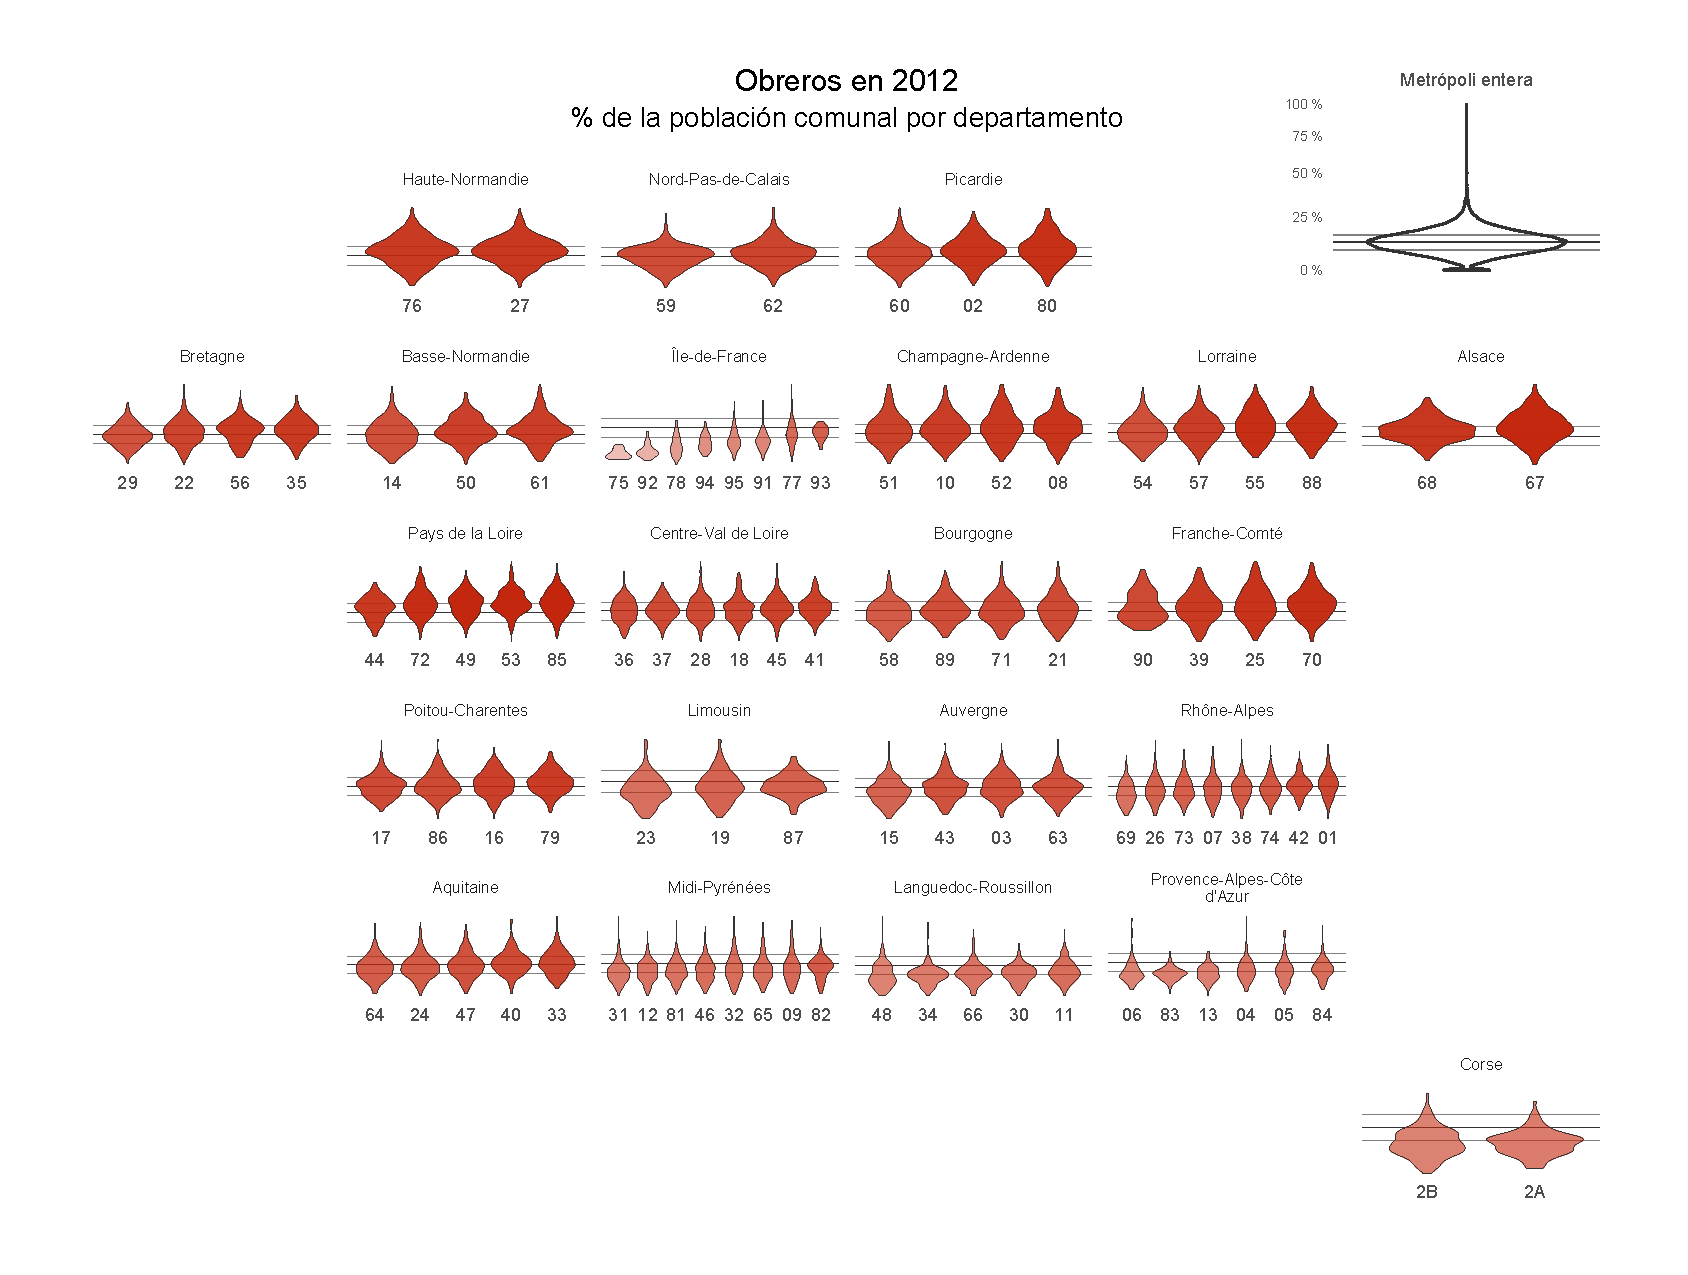
\includegraphics[width = \textwidth]{Figs/AED/Geofacet_Distr_por_Dpto_CSP6_2012}
	\end{subfigure}
	~
	\begin{subfigure}{0.235\textwidth}
	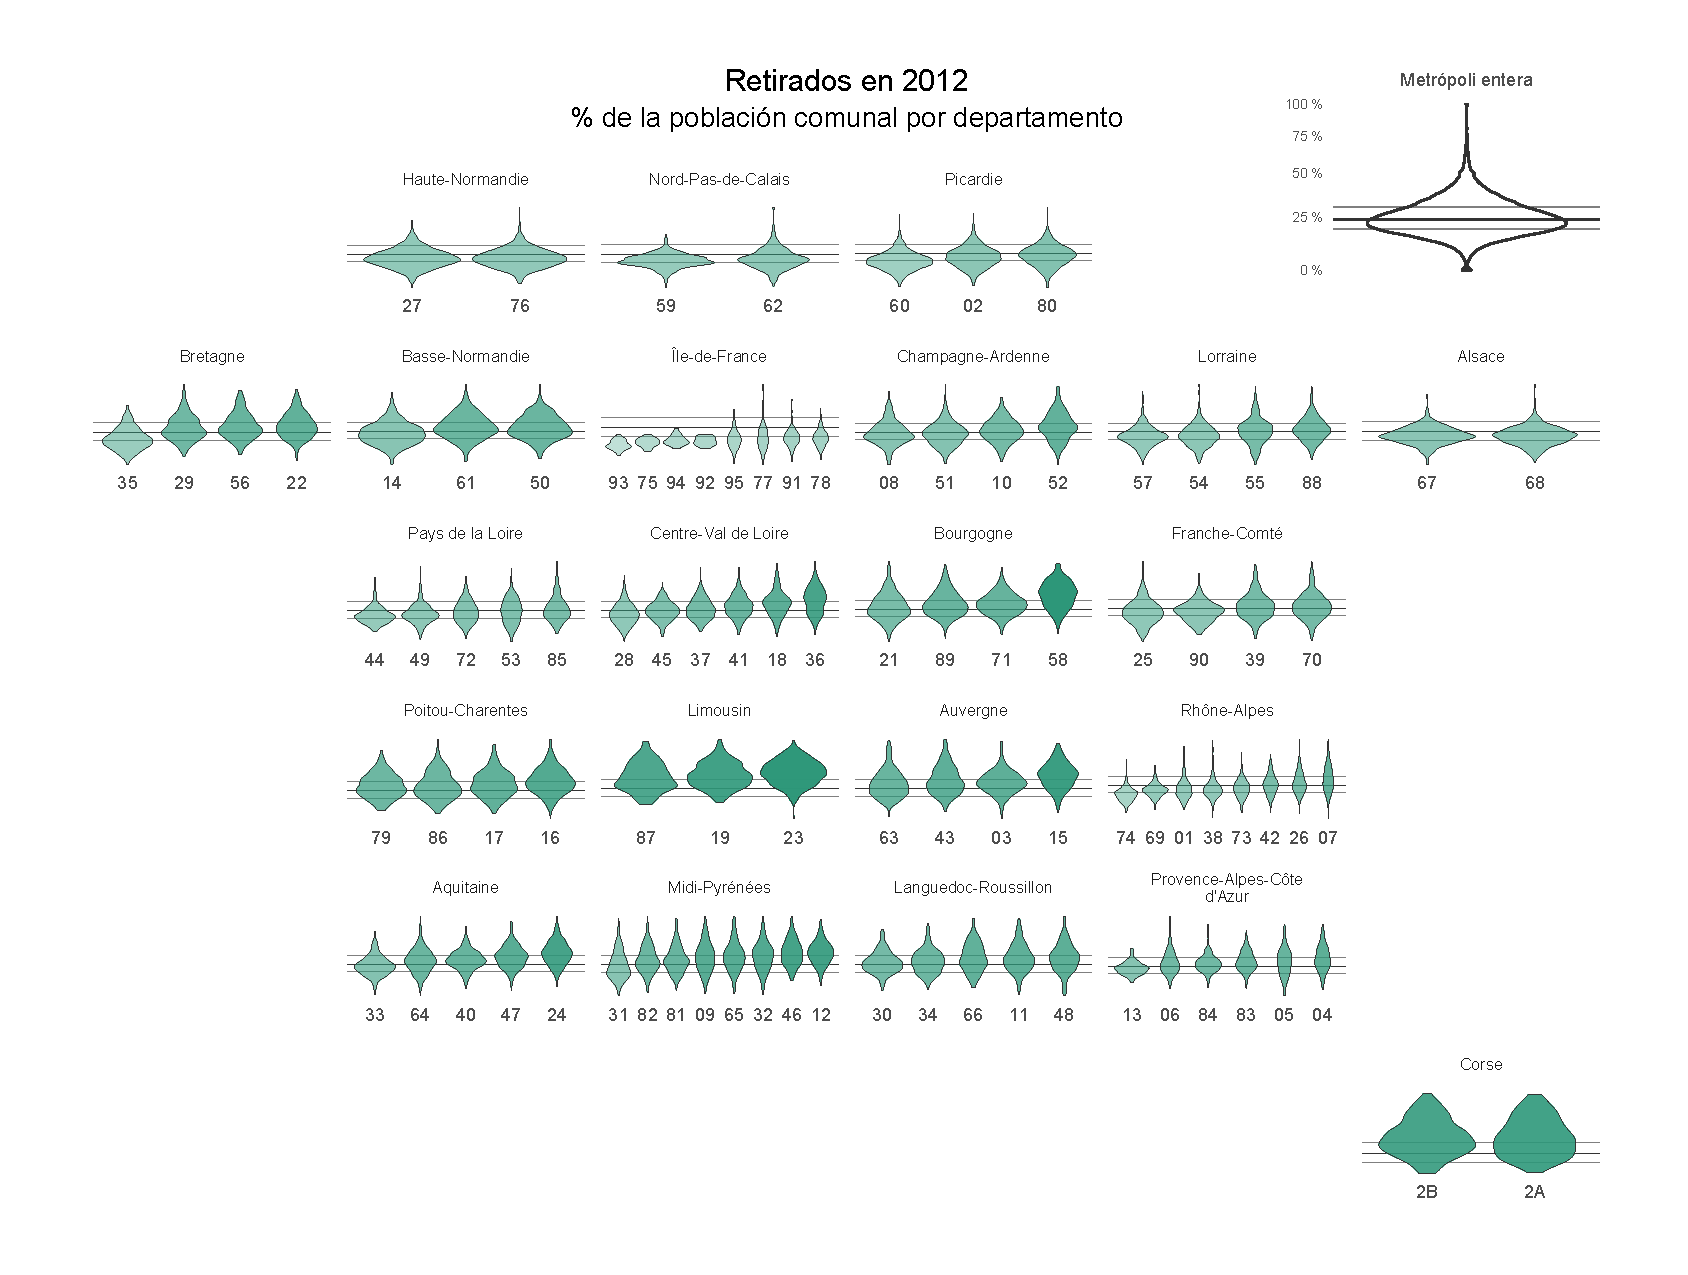
\includegraphics[width = \textwidth]{Figs/AED/Geofacet_Distr_por_Dpto_CSP7_2012}
	\end{subfigure}
	~
	\begin{subfigure}{0.235\textwidth}
	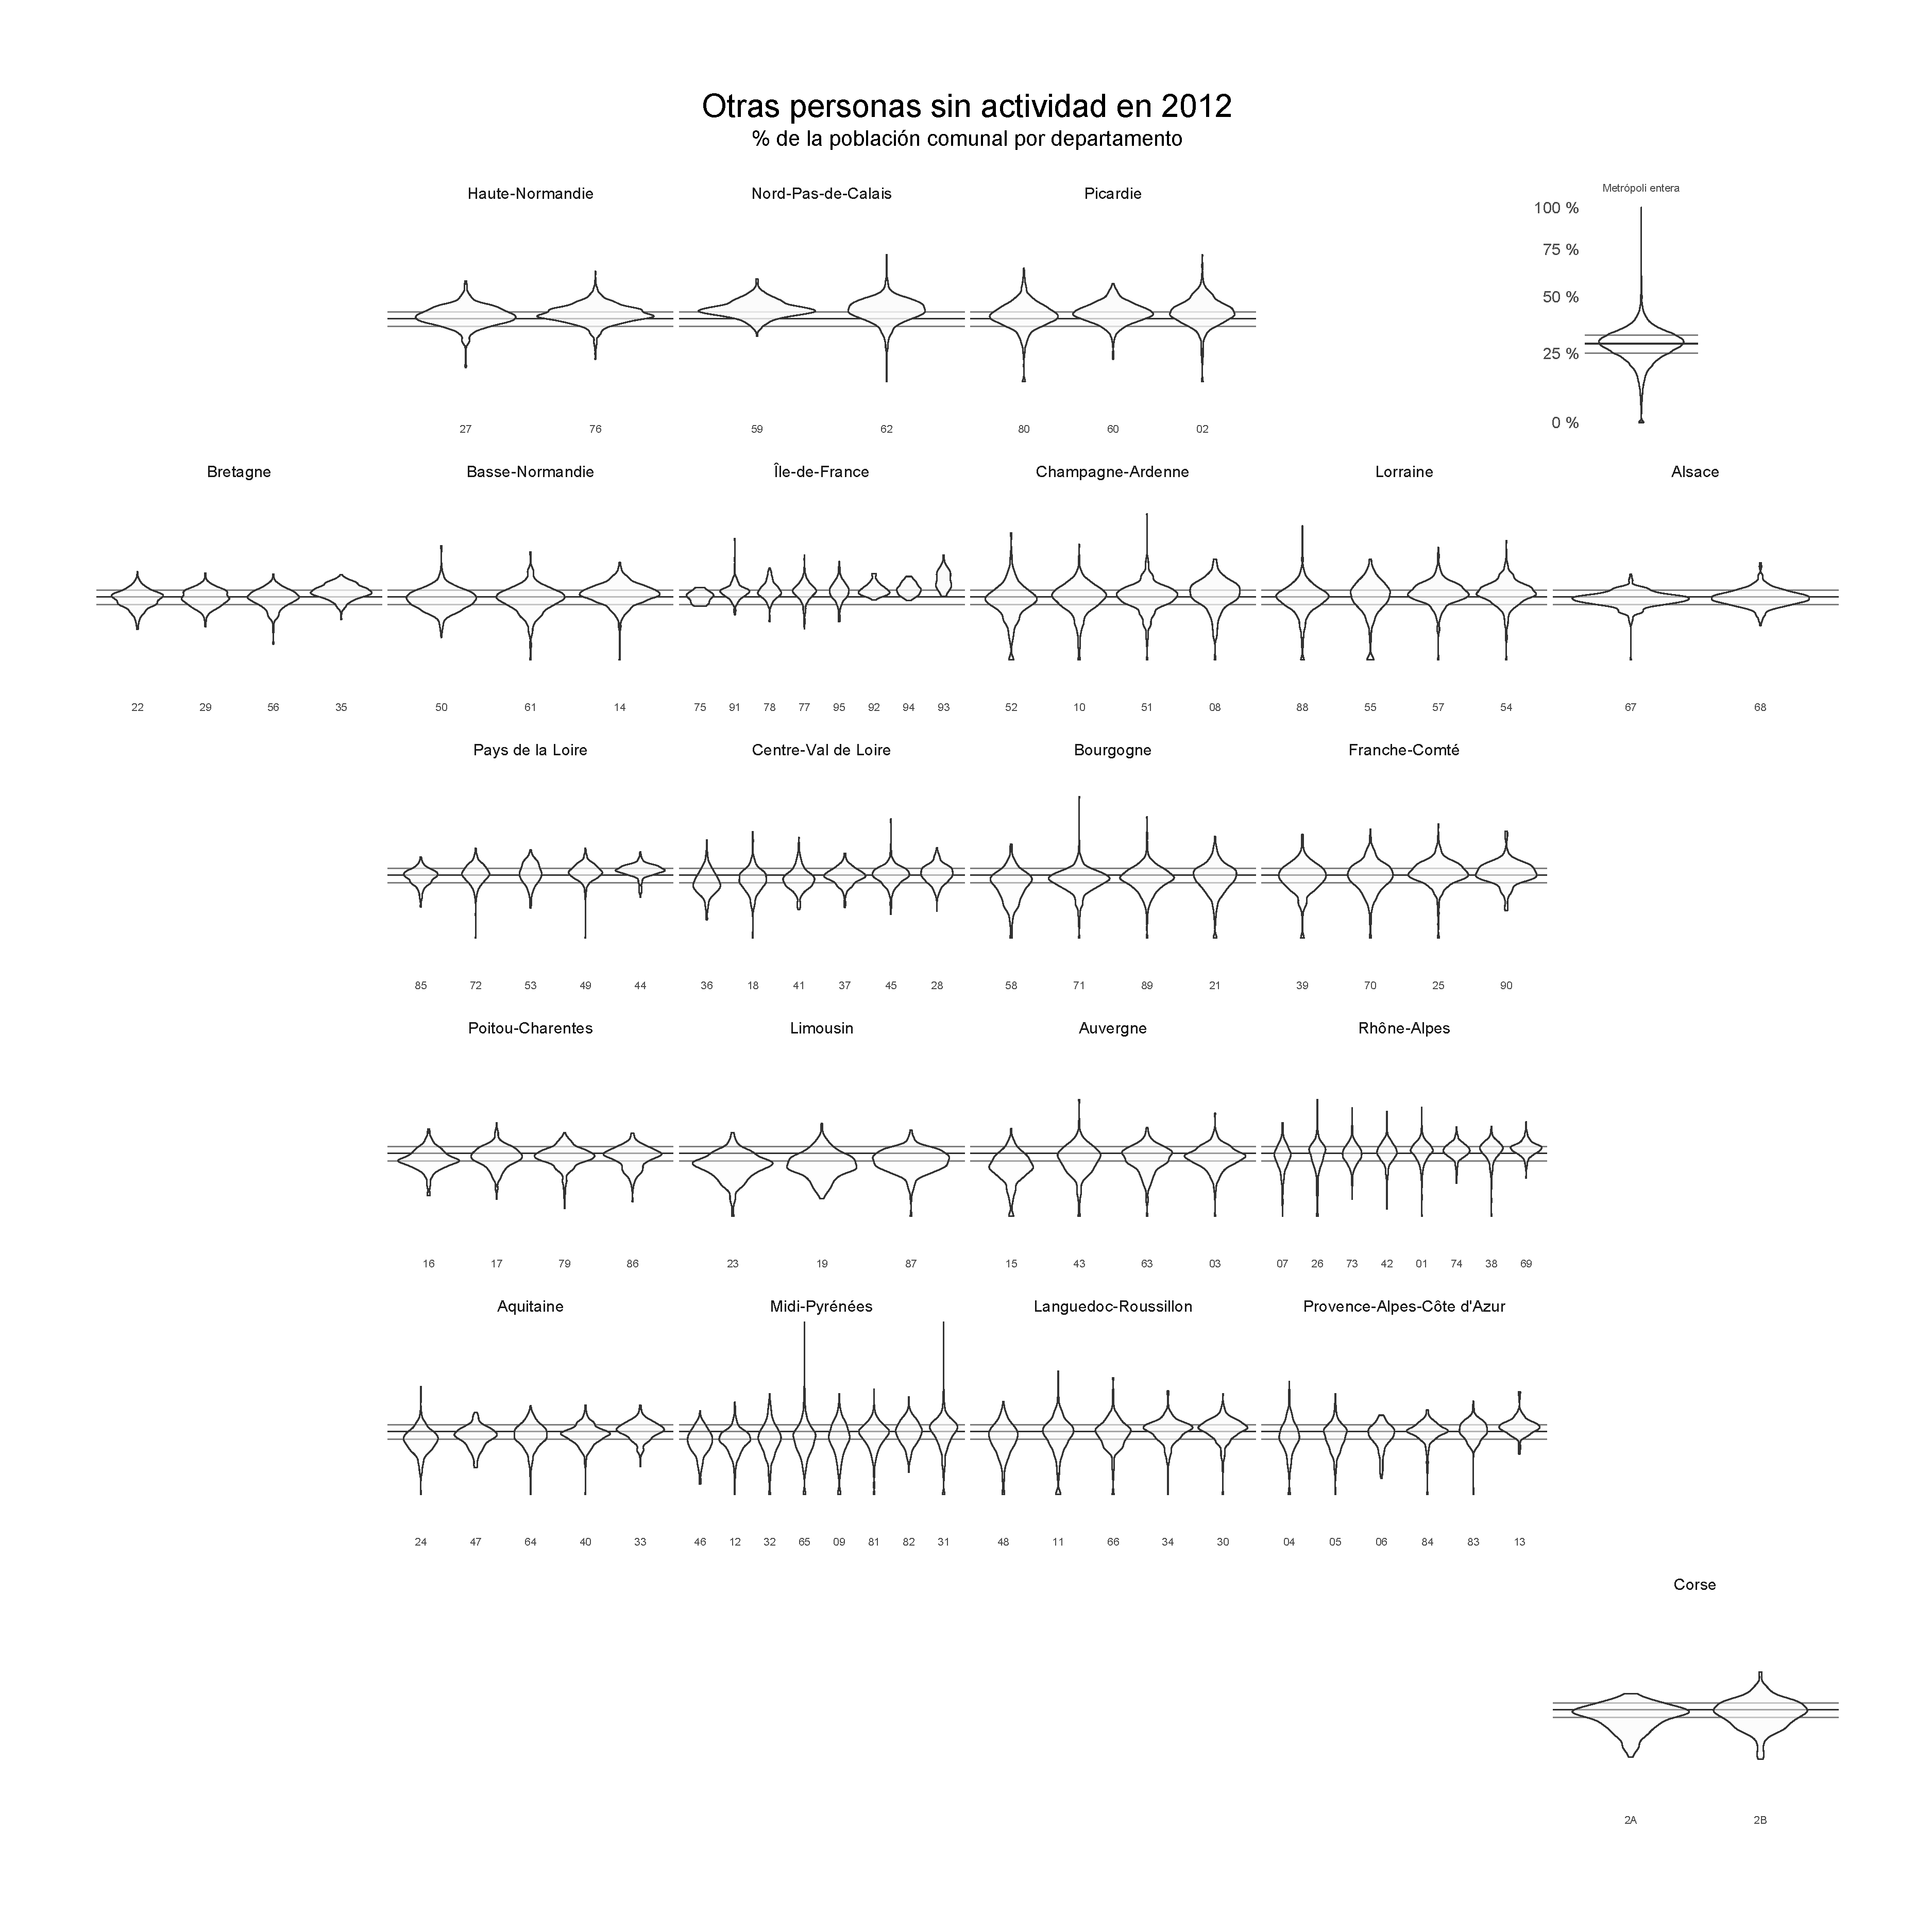
\includegraphics[width = \textwidth]{Figs/AED/Geofacet_Distr_por_Dpto_CSP8_2012}
	\end{subfigure}
	\caption{Distribuciones departamentales del porcentaje de los distintos grupos de categorías socioprofesionales como proporción de la población de las comunas en 2012. Fuente: elaboración propia con los datos censales.}
	\label{fig:Distr_por_Dpto_CSP_2012}	
\end{sidewaysfigure}
 
 En el resto de la metrópoli francesa procederé a comentar categoría por categoría. Los agricultores están presentes sobre todo en las regiones centrales y sureñas. La pequeña burguesía--- es decir los artesanos, comerciantes y empresarios--- tiene presencia en general nacional, pero resaltan las regiones de la costa mediterránea como PACA y Languedoc-Rousillon. Los cuadros y las profesiones intelectuales superiores están más representadas en las grandes ciudades como son Lyon, Marsella, Toulouse, Niza o Lille--- departamentos 69 en Rhône-Alpes, 13 en PACA, 31 en Midi-Pyrénées, 06 en PACA y 59 en Nord-Pas-de-Calais respectivamente---.\\ 
 
 Las profesiones intermediarias\footnote{Este nombre se refiere a aquellas ocupaciones que fungen como intermediarios entre personas. La mayoría son intermediarios entre gerentes y el grueso de los obreros o empleados. Otros son intermediarios en un sentido figurado, como la enfermería o el trabajo social.} tienen una variabilidad intraregional que se puede observar por la progresión de intensidades en los colores de los violines; es decir, dentro de cada región tienden a haber departamentos con medianas superiores a la mediana nacional y otros con medianas inferiores. Los empleados, por el contrario, parecen distribuirse de manera relativamente homogénea a través de los departamentos de una misma región, salvo por algunas comunas atípicas que alargan las colas de algunos violines. El norte industrial es visible desde las distribuciones de los obreros, quienes están más presentes en las regiones del norte y oeste que en el sureste.\\
 
  Las distribuciones de las proporciones de las poblaciones que representan las personas retiradas permite confirmar que el sur de Francia está más avejentado que el norte, aunque también observamos que dentro de algunas regiones como Aquitaine, Midi-Pyrénées o Bourgogne existe considerable variabilidad a través de sus departamentos. Finalmente, la categoría de personas sin actividad es más bien residual y un poco más difícil de interpretar en este nivel, pues incorpora tanto menores de edad como personas sin trabajo, incluidos estudiantes. Podemos, sin embargo, observar similitudes con las distribuciones de los menores de edad y seguir pensando que las regiones del norte tienen una estructura más juvenil que regiones más avejentadas como Limousin y Auvergne.

\clearpage
\section{Otros datos a nivel comuna}

Derivado del marco teórico sobre el voto NAP existen otras variables explicativas de interés que ayuden a perfilar el clivaje de escolaridad o el estado económico del lugar. Afortunadamente el INSEE también publica datos sobre el máximo grado escolar que tienen los habitantes mayores de 15 años de cada comuna, así como el número de habitantes que siguen estudiando.\footnote{El sistema educativo francés tiene una estructura distinta al mexicano, así que las categorías en el \textbf{Cuadro \ref{tbl:Otros_datos_comuna}} son aproximadas. Por ejemplo, entre otros, Dip2 incluye al llamado Brevet, Dip3 a varios tipos de Baccalauréat y para clasificarse en Dip4 se requieren al menos 2 años de ciclos universitarios.} Por otro lado, también es posible obtener el número de personas empleadas y desempleadas dentro de las comunas para 3 grupos de edad. La distinción por grupos de edad es importante puesto que referencias como \textcite{LeBras16} o \textcite{Perrineau07} tienden a mencionar la precariedad salarial juvenil como un catalizador del voto frontista.\\ 

\begin{table}[h]
\centering
\resizebox{\linewidth}{!}{
\begin{tabular}{|c | c | c | c |}
\hline
\textbf{Base de origen} &
\textbf{Variable} & 
\textbf{Abreviatura} & 
\textbf{Categoría}\\[2pt] 
\hline
\multirow{5}{*}{Diplômes-formation} & 
\multirow{5}{*}{Escolaridad} &  
Dip1 & Personas sin escolaridad\\ 
&& Dip2 & Primaria o secundaria\\  
&& Dip3 & Preparatoria o equivalente\\  
&& Dip4 & Universidad o más\\ 
&& Esc & Personas aún estudiando\\ \hline
\multirow{6}{*}{Emploi-population active} & 
\multirow{6}{*}{Empleo} & 
Ocu1 & Empleados de 15 a 24 años\\
&& Des1 & Desempleados de 15 a 24 años\\
&& Ocu2 & Empleados de 25 a 54 años\\
&& Des2 & Desempleados de 25 a 54 años\\
&& Ocu3 & Empleados de 55 a 64 años\\
&& Des3 & Desempleados de 55 a 64 años\\
\hline
\end{tabular}
}
\caption{Otros datos a nivel comuna a utilizar en el análisis.}
\label{tbl:Otros_datos_comuna}
\end{table}

Si repetimos el análisis exploratorio hecho para los datos censales, vemos en la \textbf{Figura \ref{fig:Distr_por_Dpto_Esc_2012}} las distribuciones departamentales por nivel escolar en 2012. En primer lugar, confirmamos la singularidad de Île de France respecto al resto del país. Es claramente la región con los departamentos más escolarizados de Francia, en el sentido de que tienden a tener una población con mayores niveles de escolarización y con diploma universitario--- notablemente en 75-París intramuros y el acaudalado 92-Hauts-de-Seine---. Asimismo, observamos menores porcentajes de personas sin ningún diploma escolar, salvo el caso aparentemente atípico de 93-Seine-Saint-Denis, pero que veíamos en la sección anterior que era el departamento de más inmigrantes, empleados y obreros. Resulta ilustrativo el patrón de personas con preparatoria pues hay un contraste entre París y su \textit{petite courone} y la \textit{grande courone}--- 75, 92, 93 y 94 vs 78, 95, 91 y 77---.\\ 

 Respecto al panorama general de la metrópoli, de nueva cuenta se refleja el patrón generacional de un norte más joven que el sur observando las distribuciones de personas todavía estudiando. Resaltan departamentos en Corse, Poitou-Charentes, Basse-Normandie o Picardie como lugares con altas poblaciones no escolarizadas. Por su parte, Limousin, Auvergne, Champagne-Ardenne y, en cierto sentido, Midi-Pyrinées son regiones con fuertes poblaciones cuyo máximo nivel de estudios es la educación básica.\\ 
 
 En cuanto a las personas con preparatoria, ambos departamentos en Alsace se ubican por encima de la mediana nacional. En términos de población con diploma universitario encontramos lugares cercanos a grandes universidades francesas como la de Aix-Marsaille, 13 en PACA, o en Rhône-Alpes las de Grenoble-Alpes (38) y la ENS-Lyon (69). También en dicha región resalta que el departamento con mayor mediana es 74-Haute-Savoie, probablemente se debe a su carácter conurbado con la ciudad suiza de Ginebra.\\
 
\begin{figure}[h]
	\centering
	\begin{subfigure}{0.3\textwidth}
	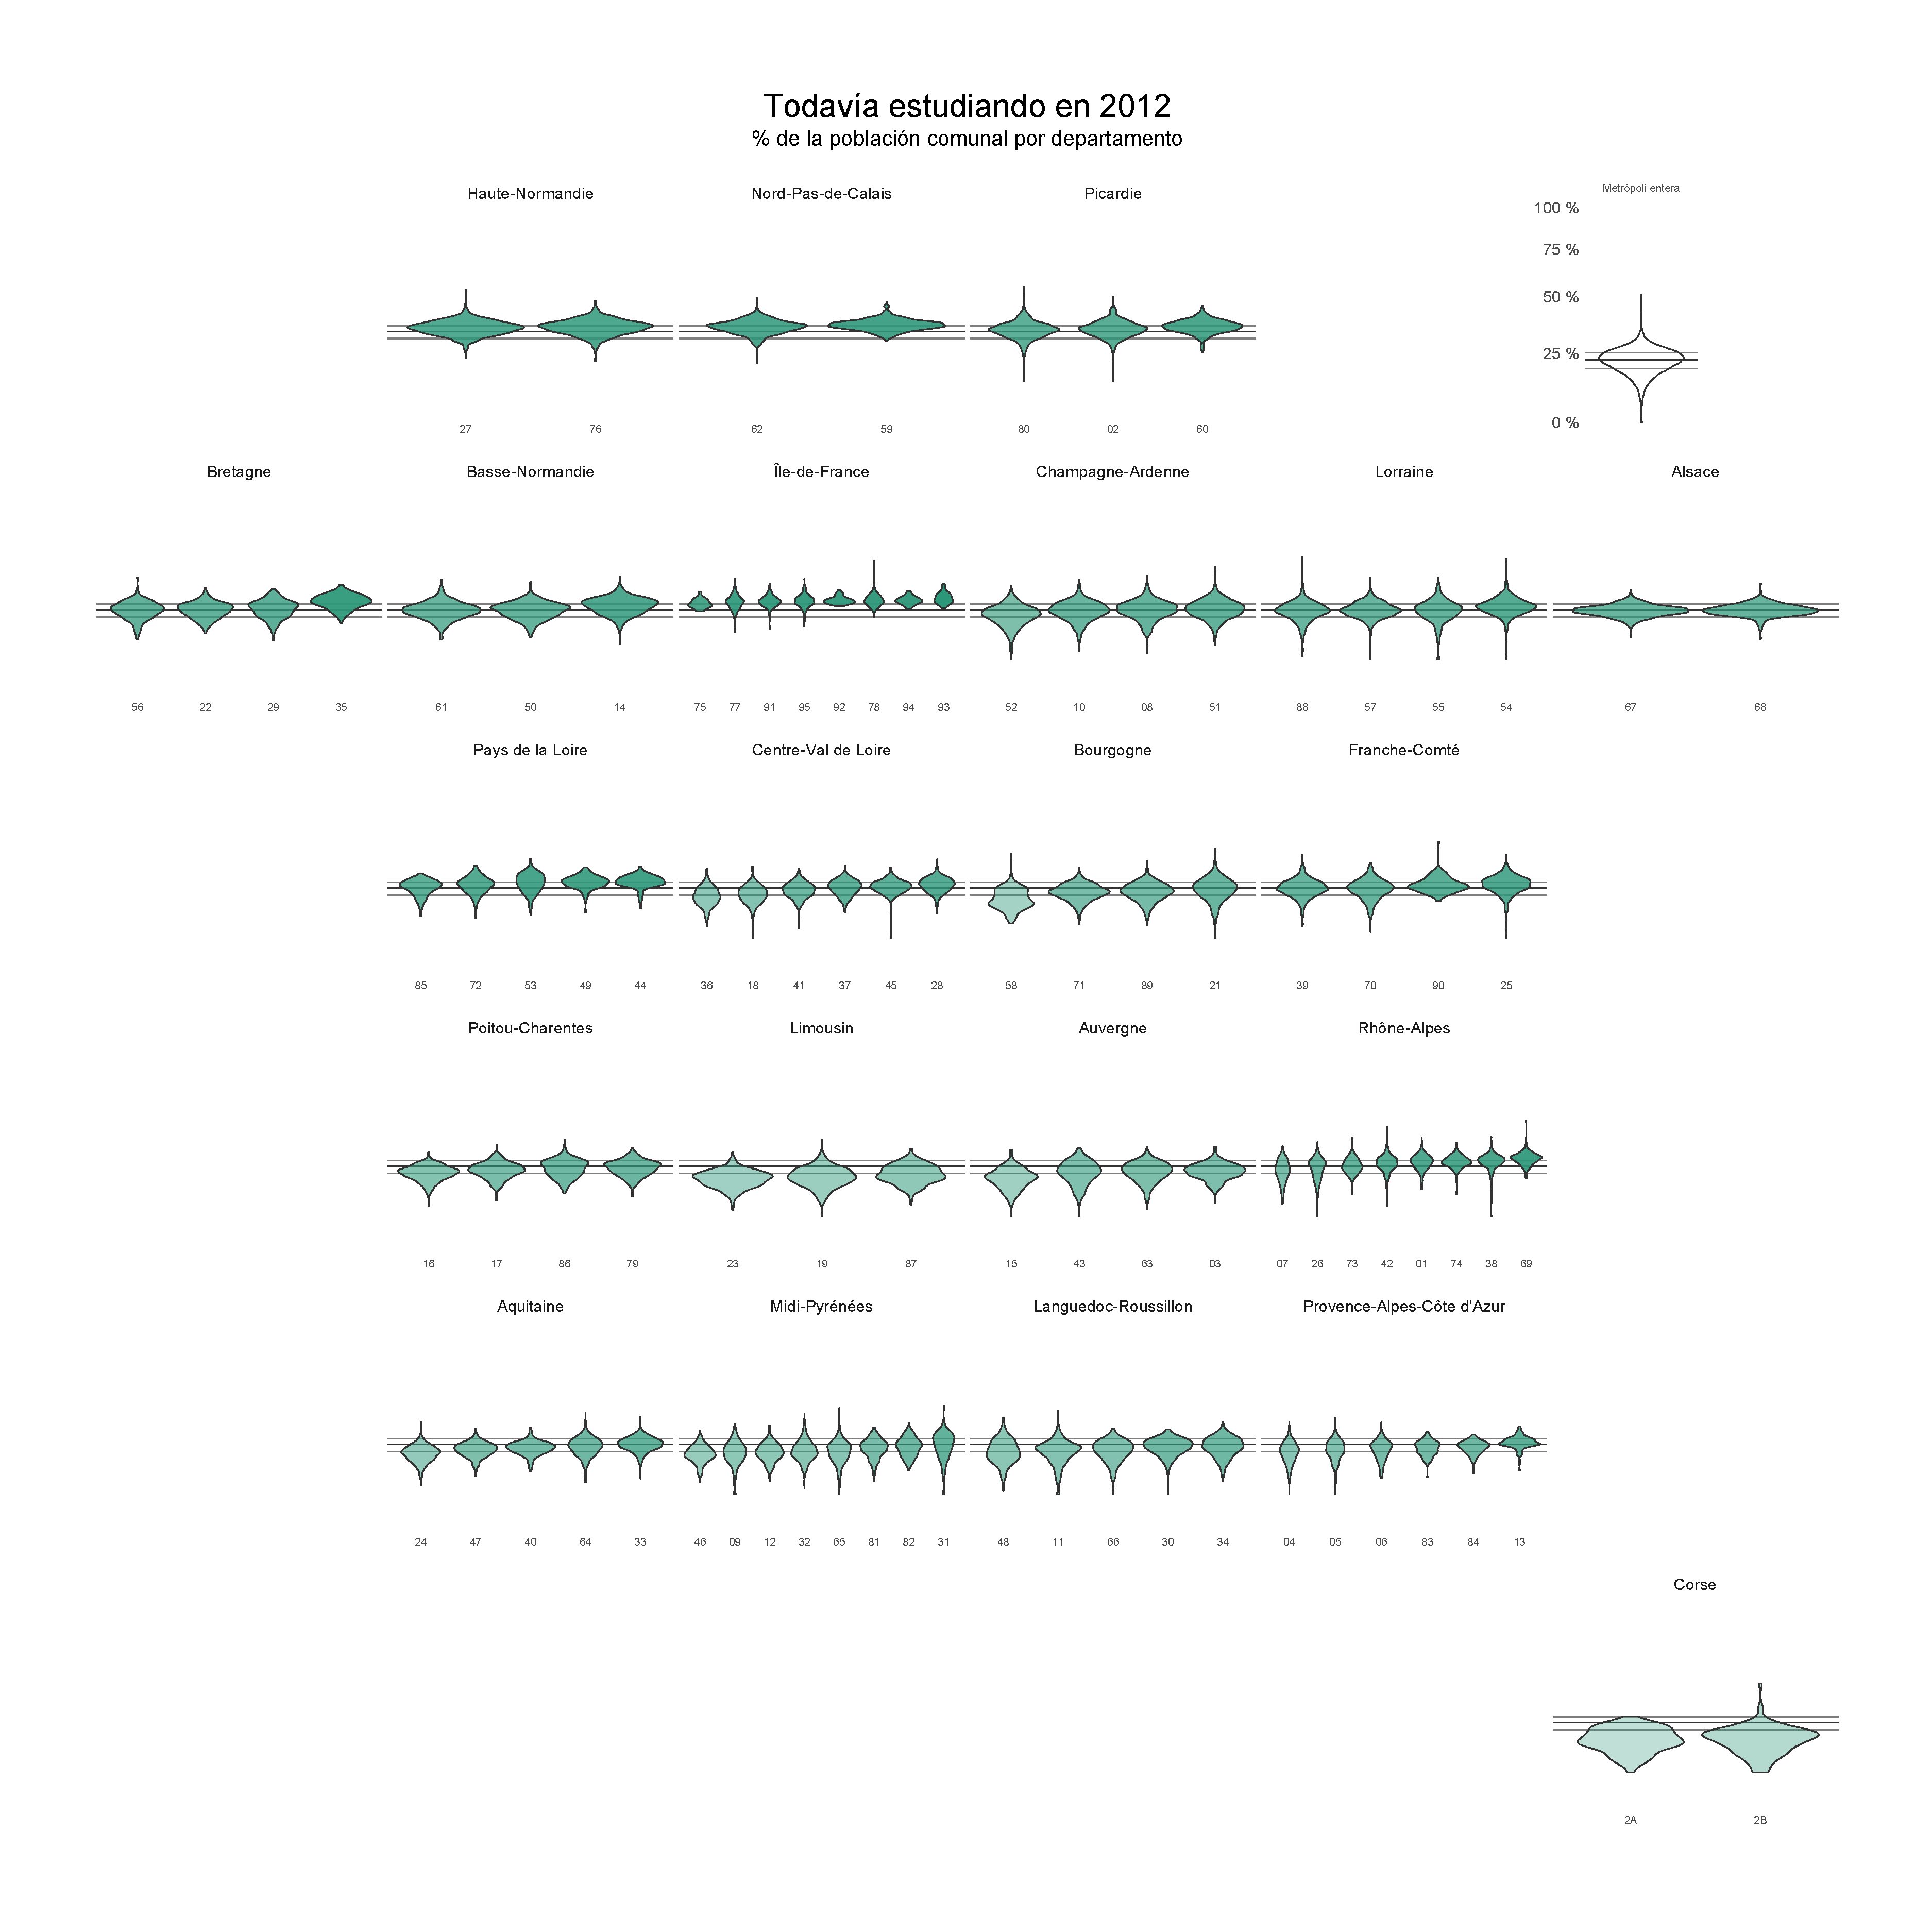
\includegraphics[width = \textwidth]{Figs/AED/Geofacet_Distr_por_Dpto_Esc_2012}
	\end{subfigure}
	~
	\begin{subfigure}{0.3\textwidth}
	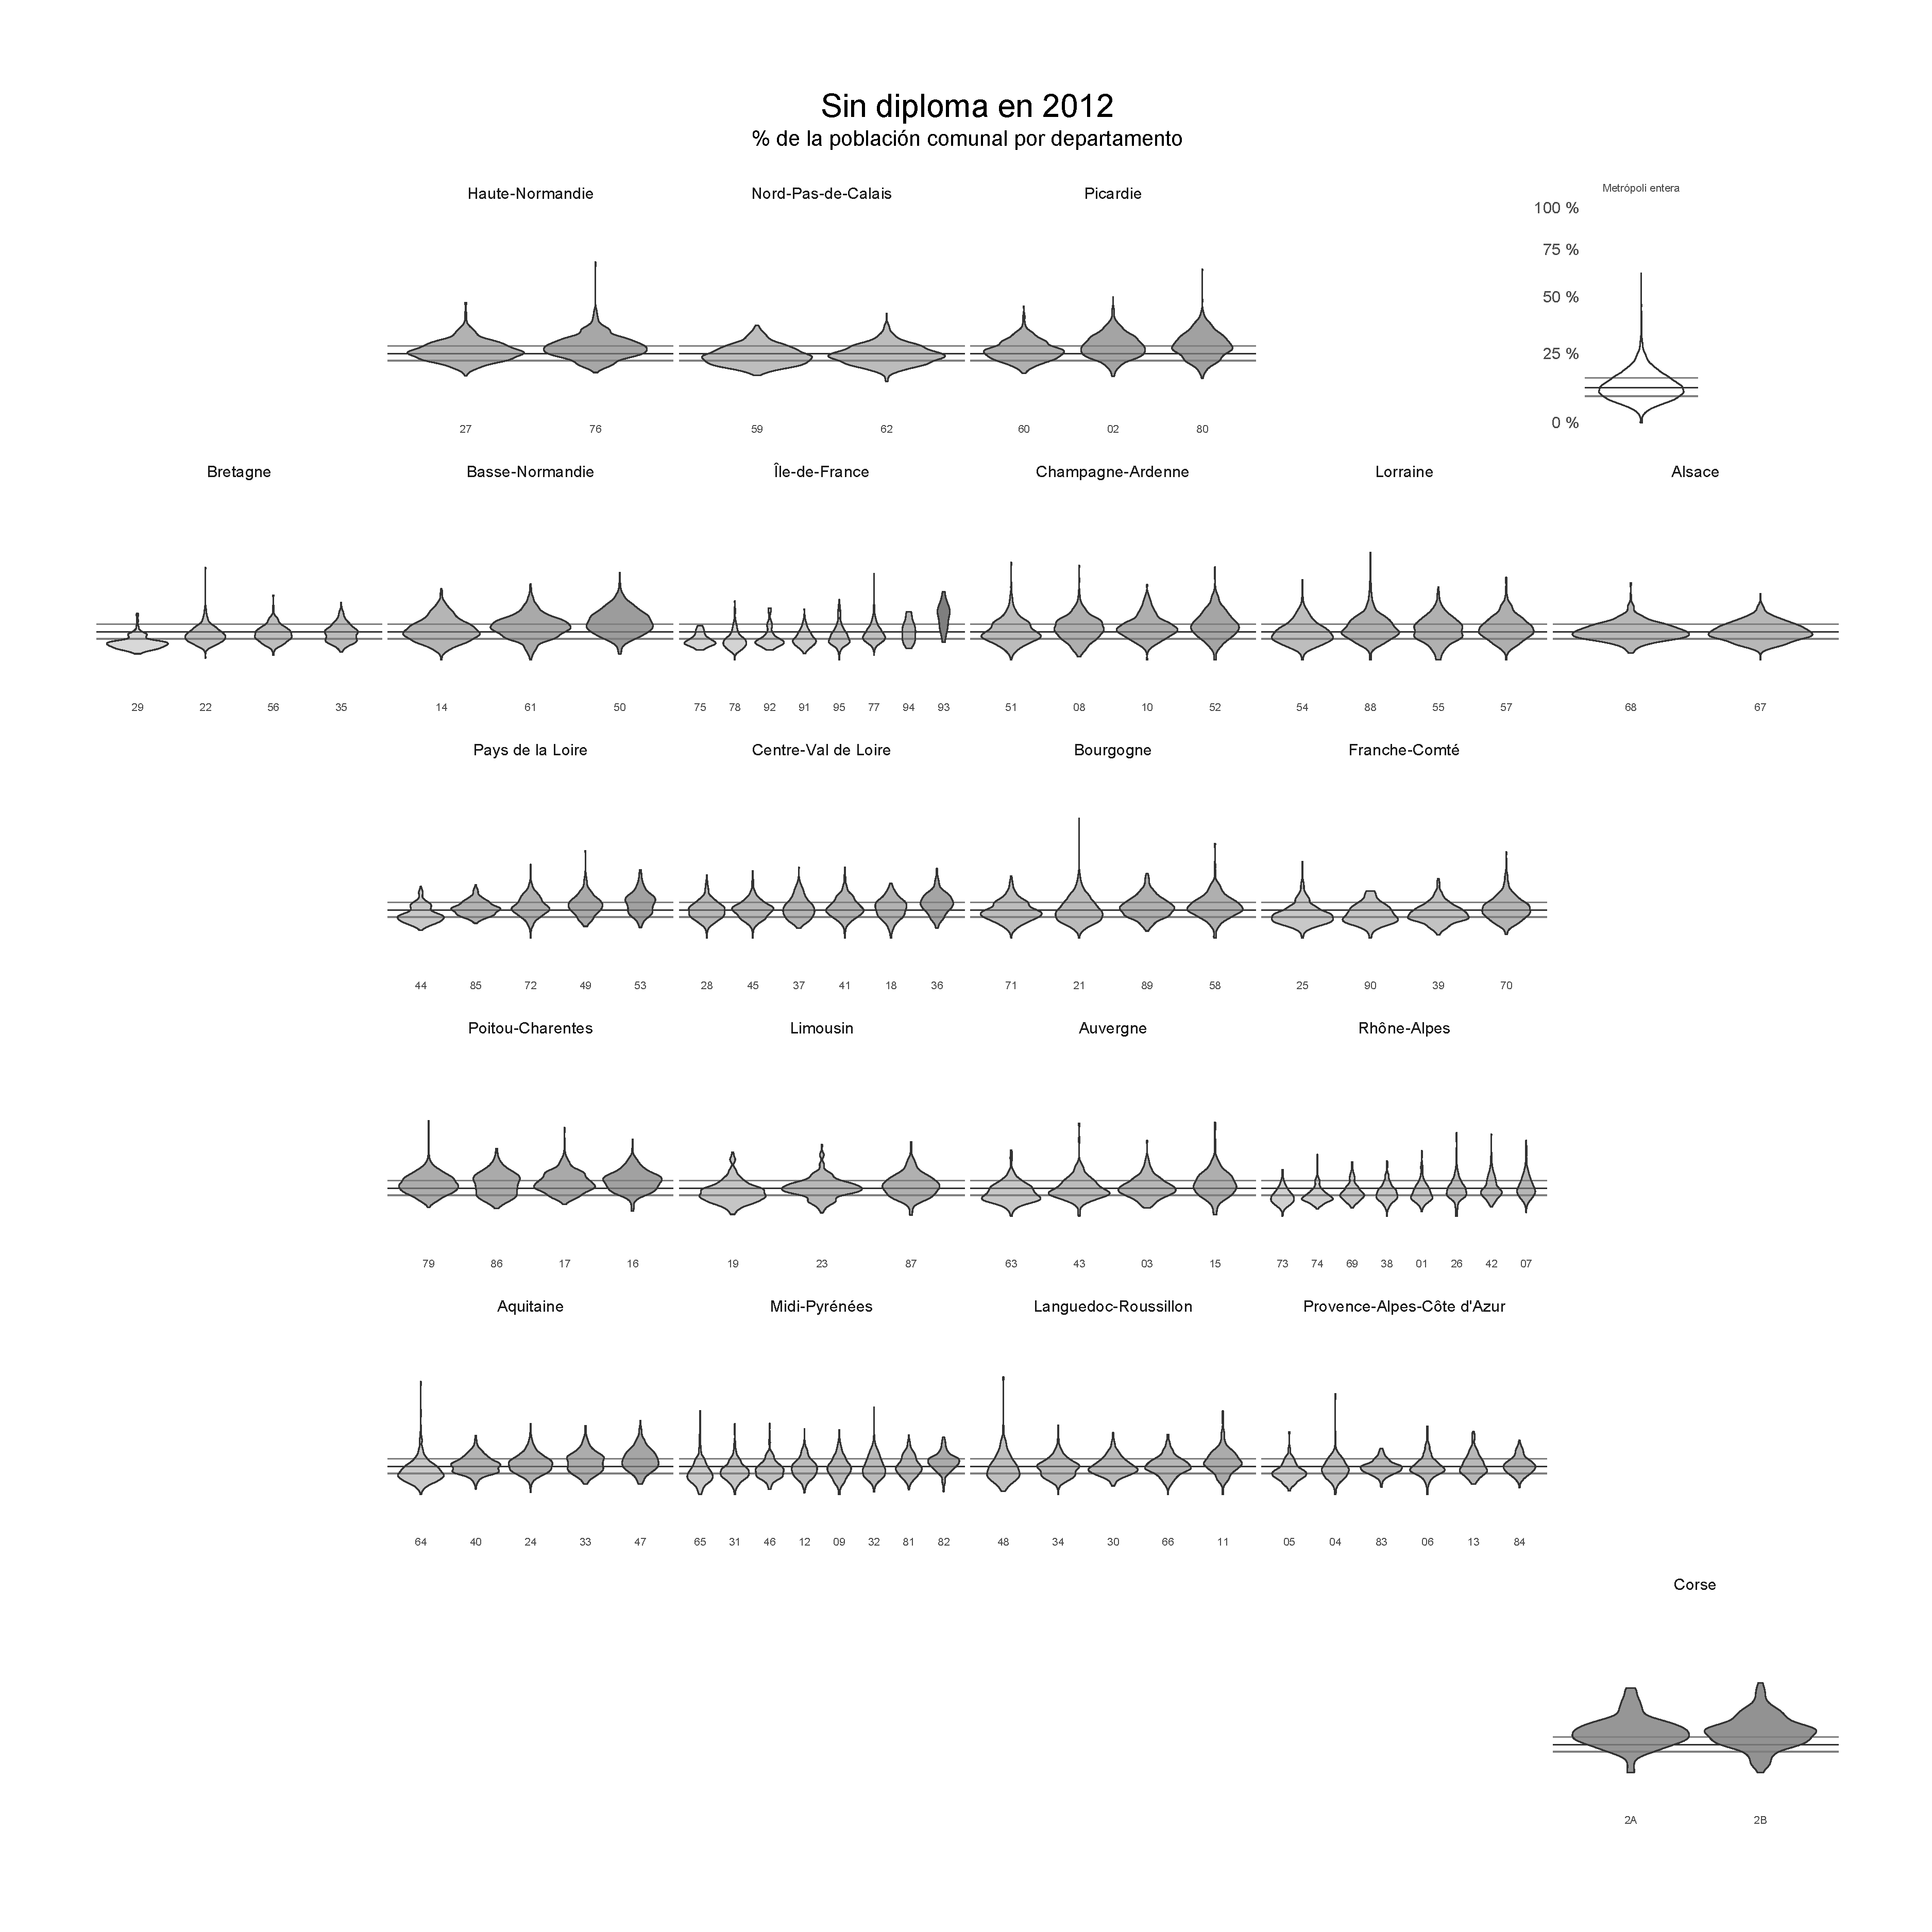
\includegraphics[width = \textwidth]{Figs/AED/Geofacet_Distr_por_Dpto_Dip1_2012}
	\end{subfigure}\\
	\begin{subfigure}{0.3\textwidth}
	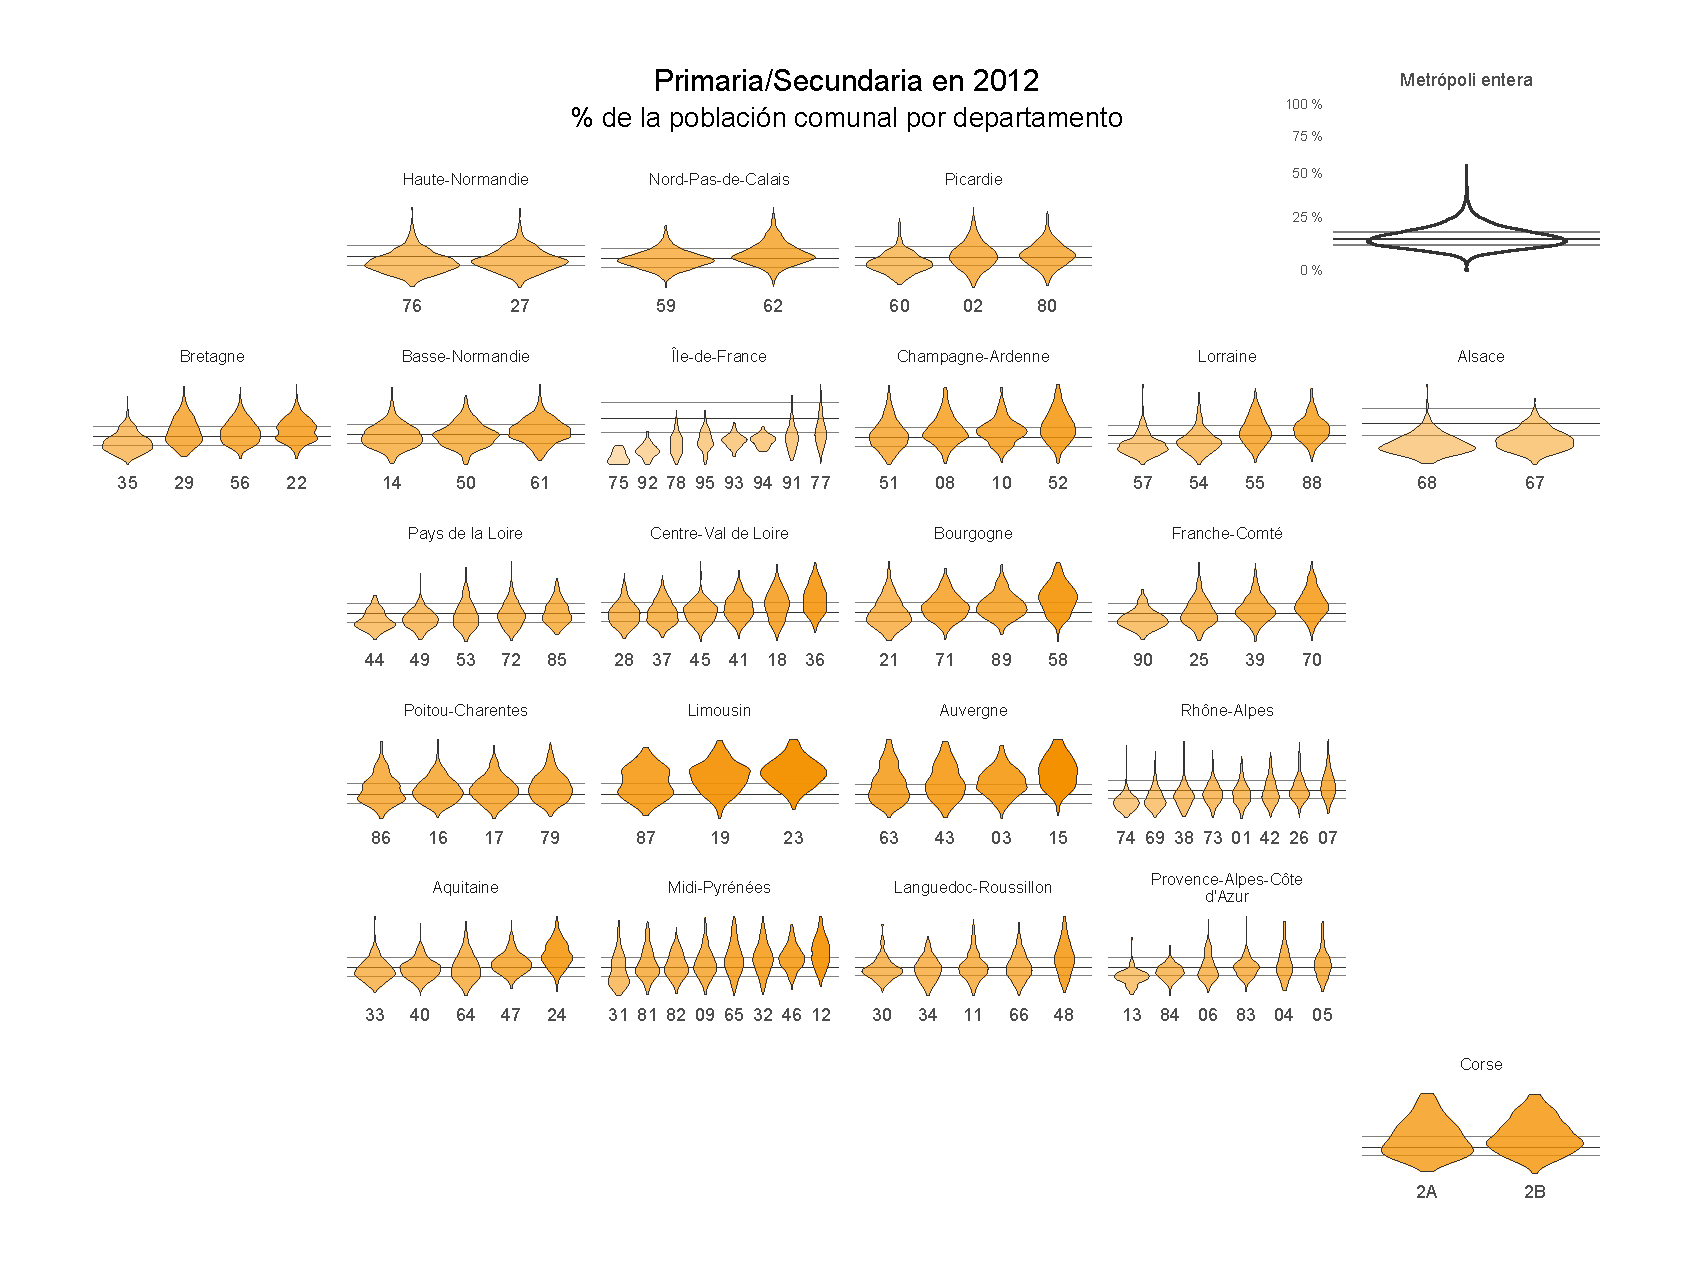
\includegraphics[width = \textwidth]{Figs/AED/Geofacet_Distr_por_Dpto_Dip2_2012}
	\end{subfigure}
	~
	\begin{subfigure}{0.3\textwidth}
	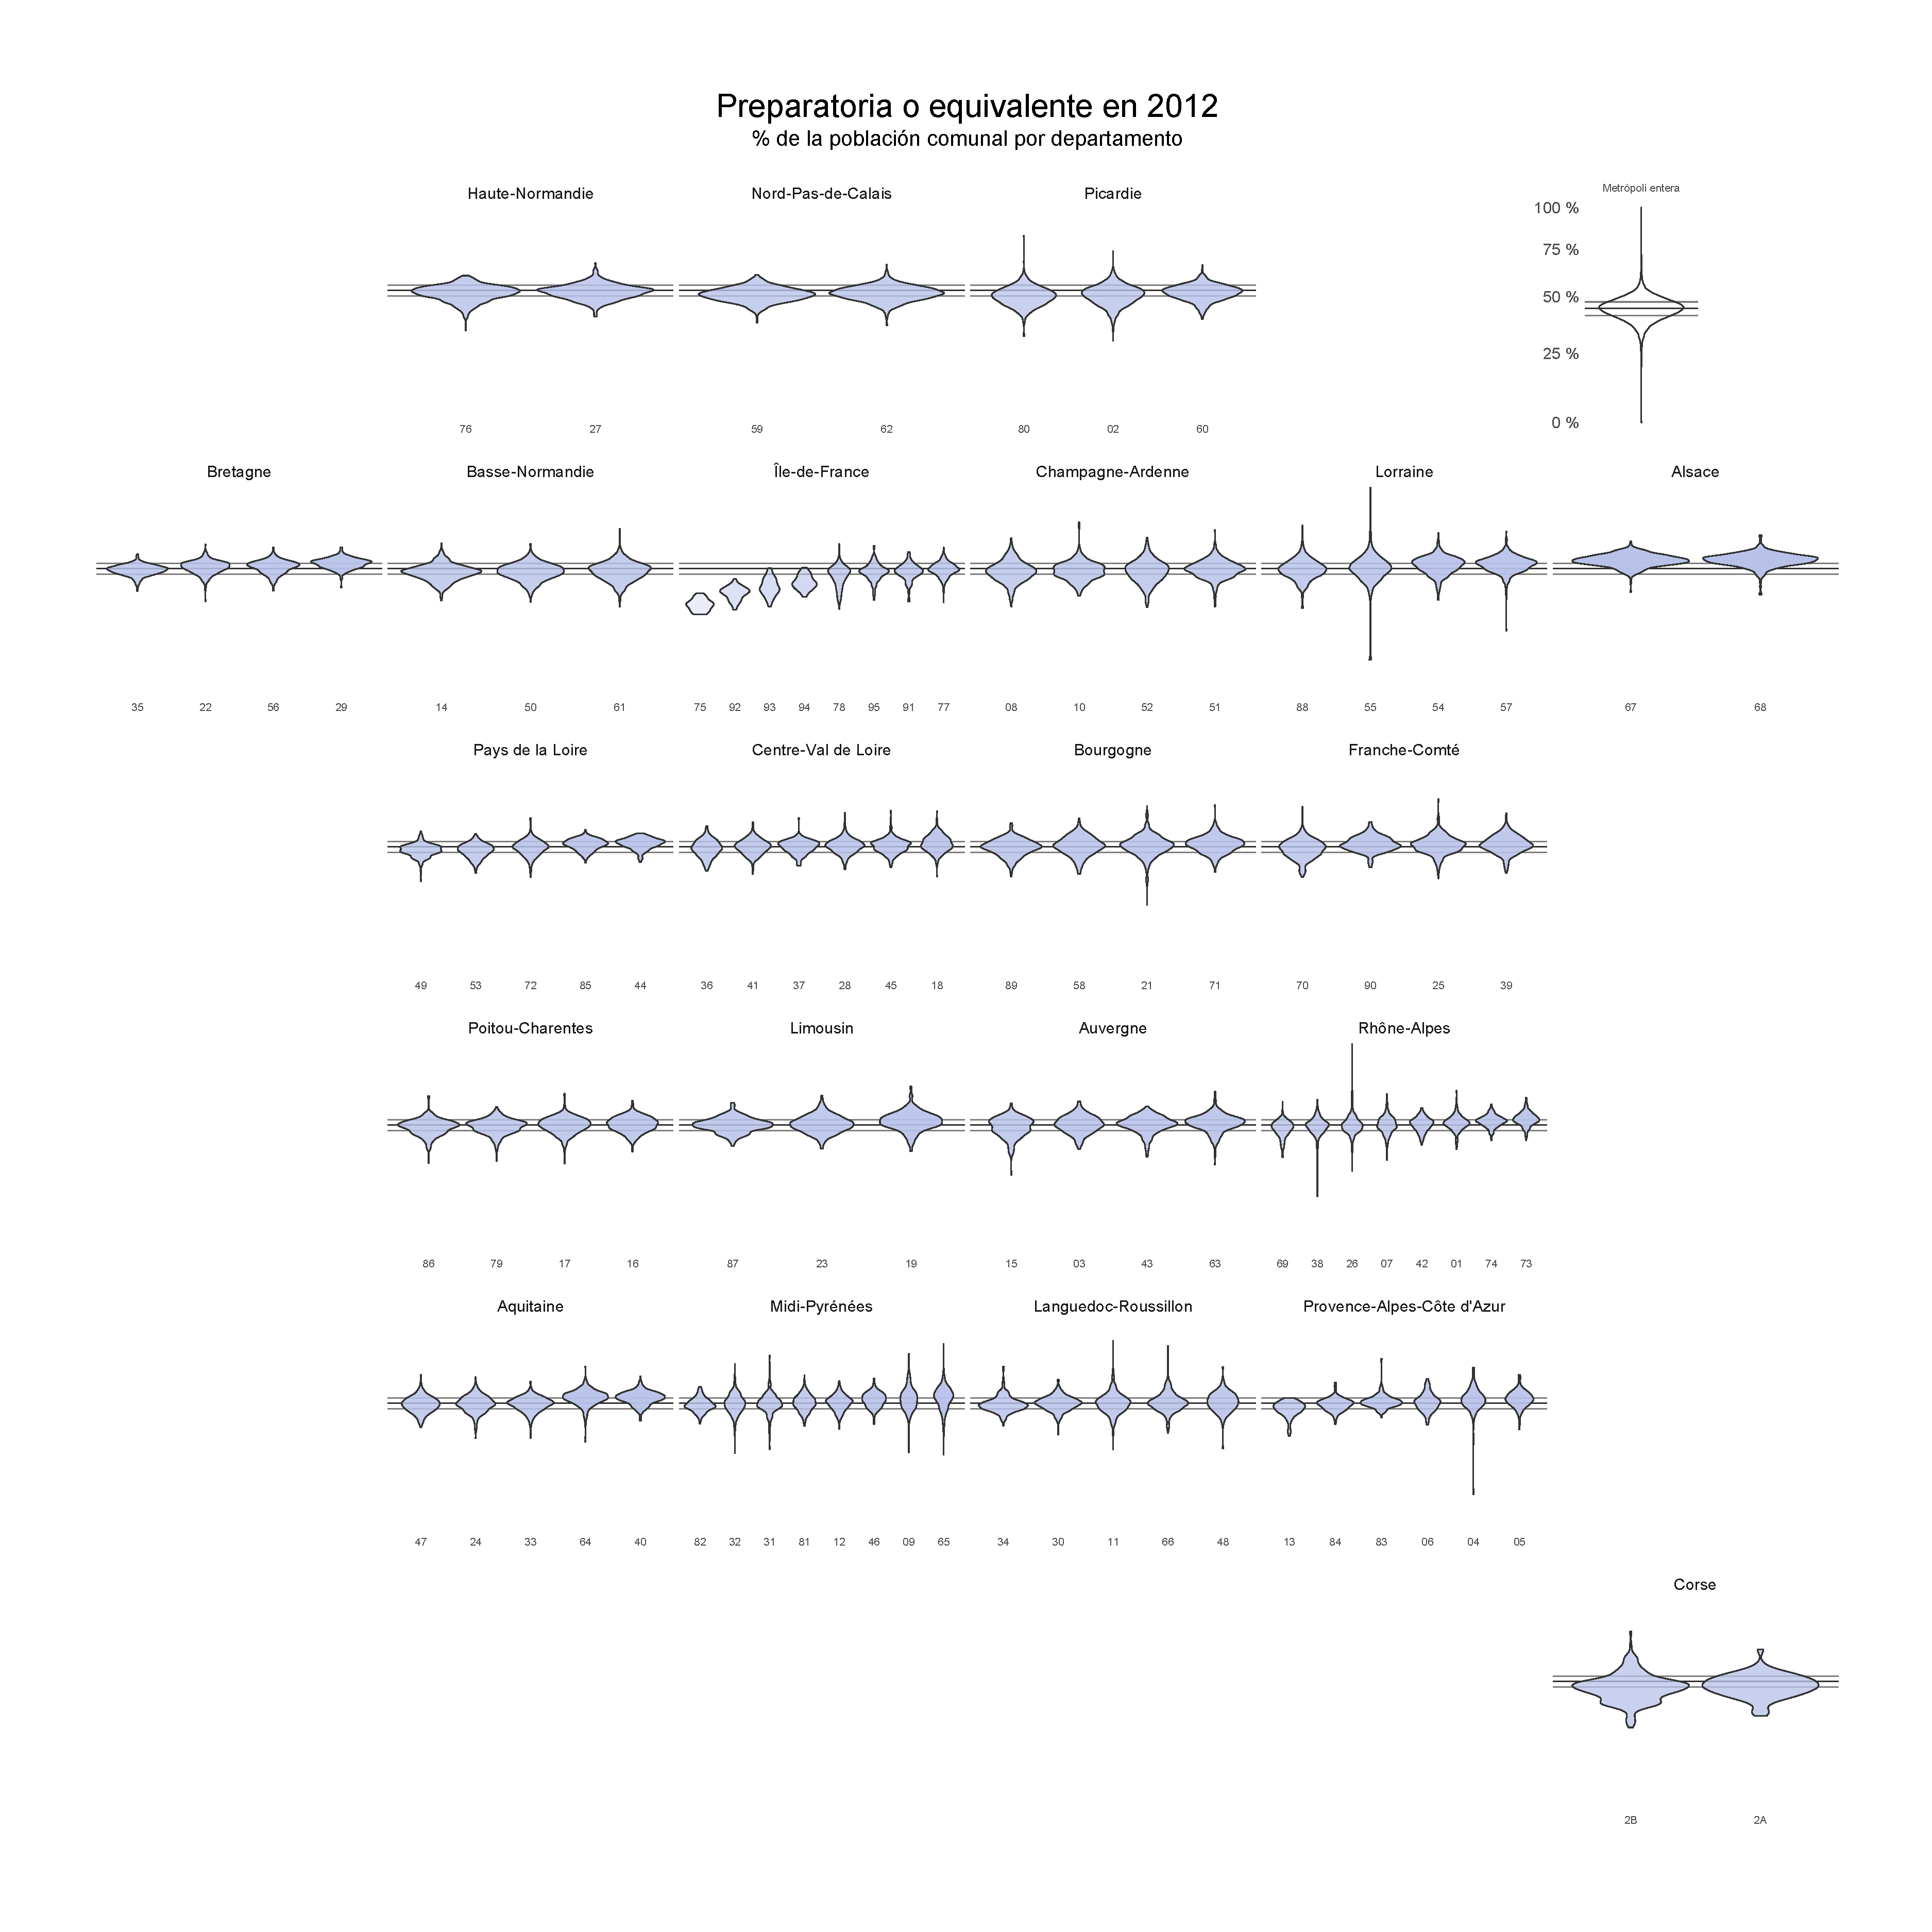
\includegraphics[width = \textwidth]{Figs/AED/Geofacet_Distr_por_Dpto_Dip3_2012}
	\end{subfigure}
	~
	\begin{subfigure}{0.3\textwidth}
	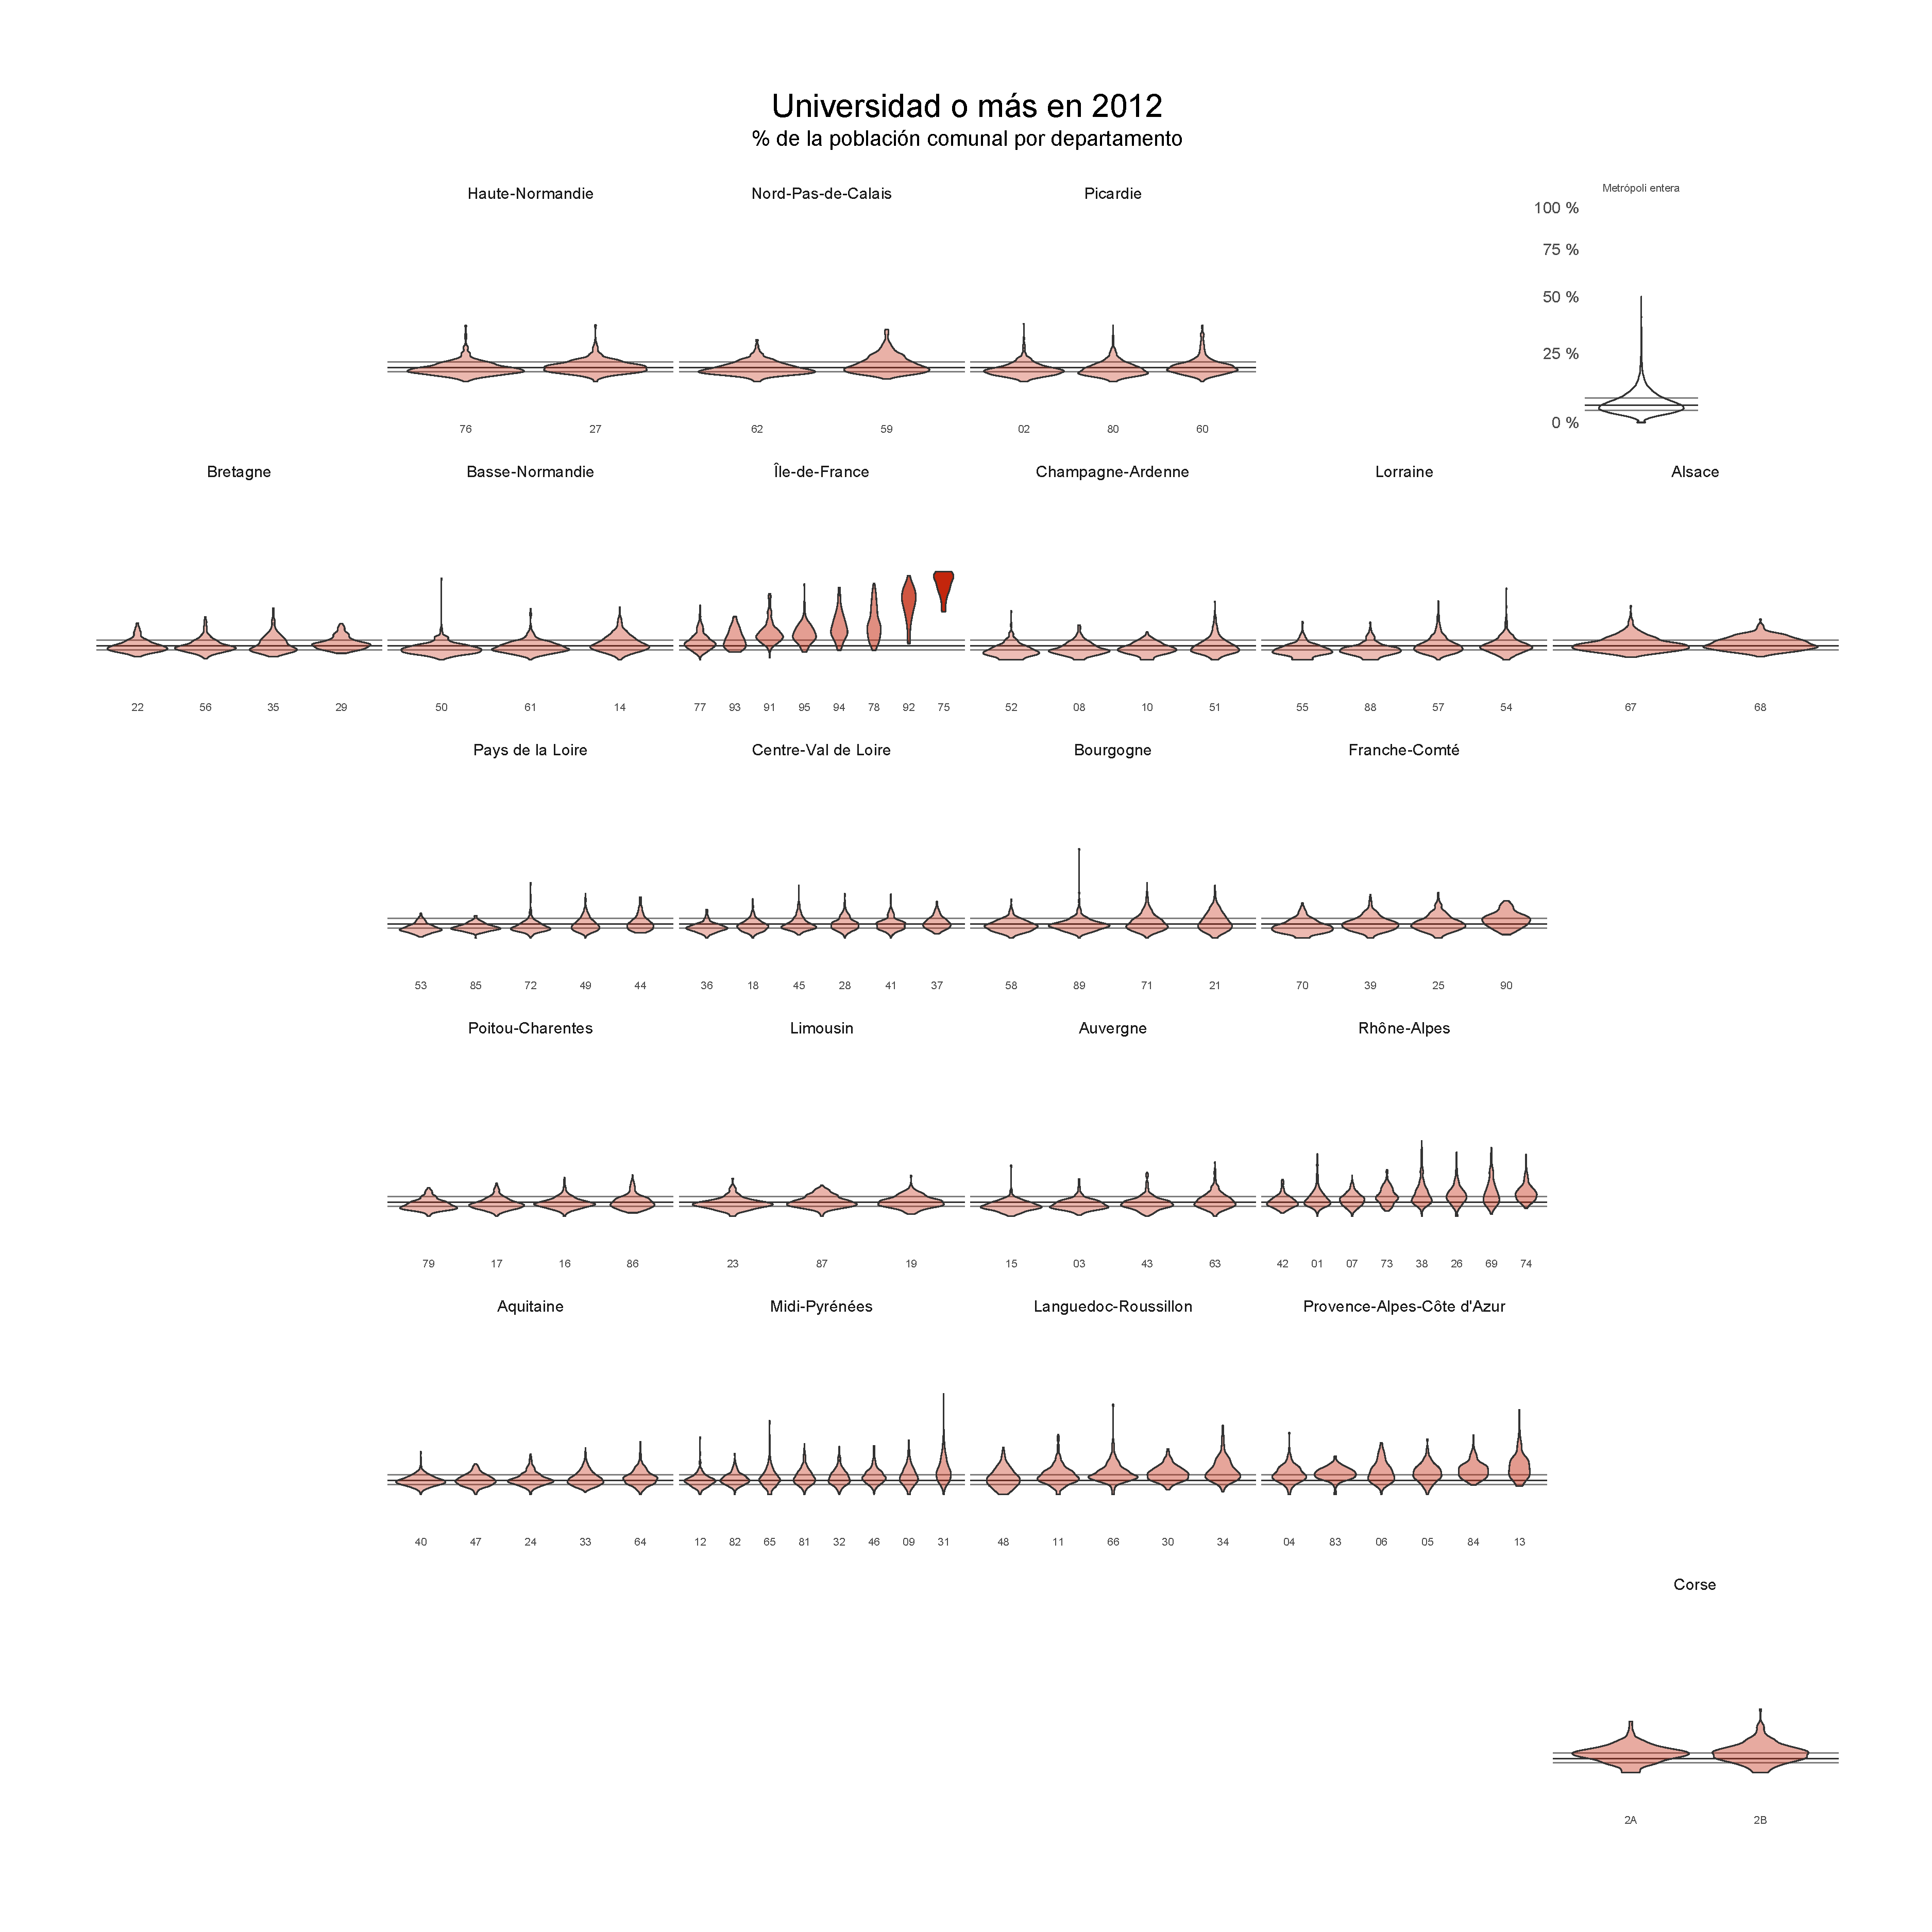
\includegraphics[width = \textwidth]{Figs/AED/Geofacet_Distr_por_Dpto_Dip4_2012}
	\end{subfigure}
	\caption{Distribuciones departamentales del porcentaje de los distintos grupos de escolaridad como proporción de la población de las comunas en 2012. Fuente: elaboración propia con los datos del INSEE.}
	\label{fig:Distr_por_Dpto_Esc_2012}	
\end{figure}

En el caso del empleo, para cada grupo de edad, contamos con el porcentaje de desempleados y su complemento. Bastan presentarse entonces los gráficos para los desempleados en la \textbf{Figura \ref{fig:Distr_por_Dpto_Ocu_2012}}. Lo primero que llama la atención es el rango de variabilidad del porcentaje de desempleados juveniles. Mientras que en el resto de variables aquí consideradas las comunas que llegan a tener valores de 0 o 100 por ciento son más bien casos atípicos en las colas de las distribuciones, en la distribución nacional de desempleo juvenil observamos modas en 0 y en 100. Este carácter multimodal se conserva en la mayoría de los departamentos.\\ 

\begin{figure}[H]
	\centering
	\begin{subfigure}{0.3\textwidth}
	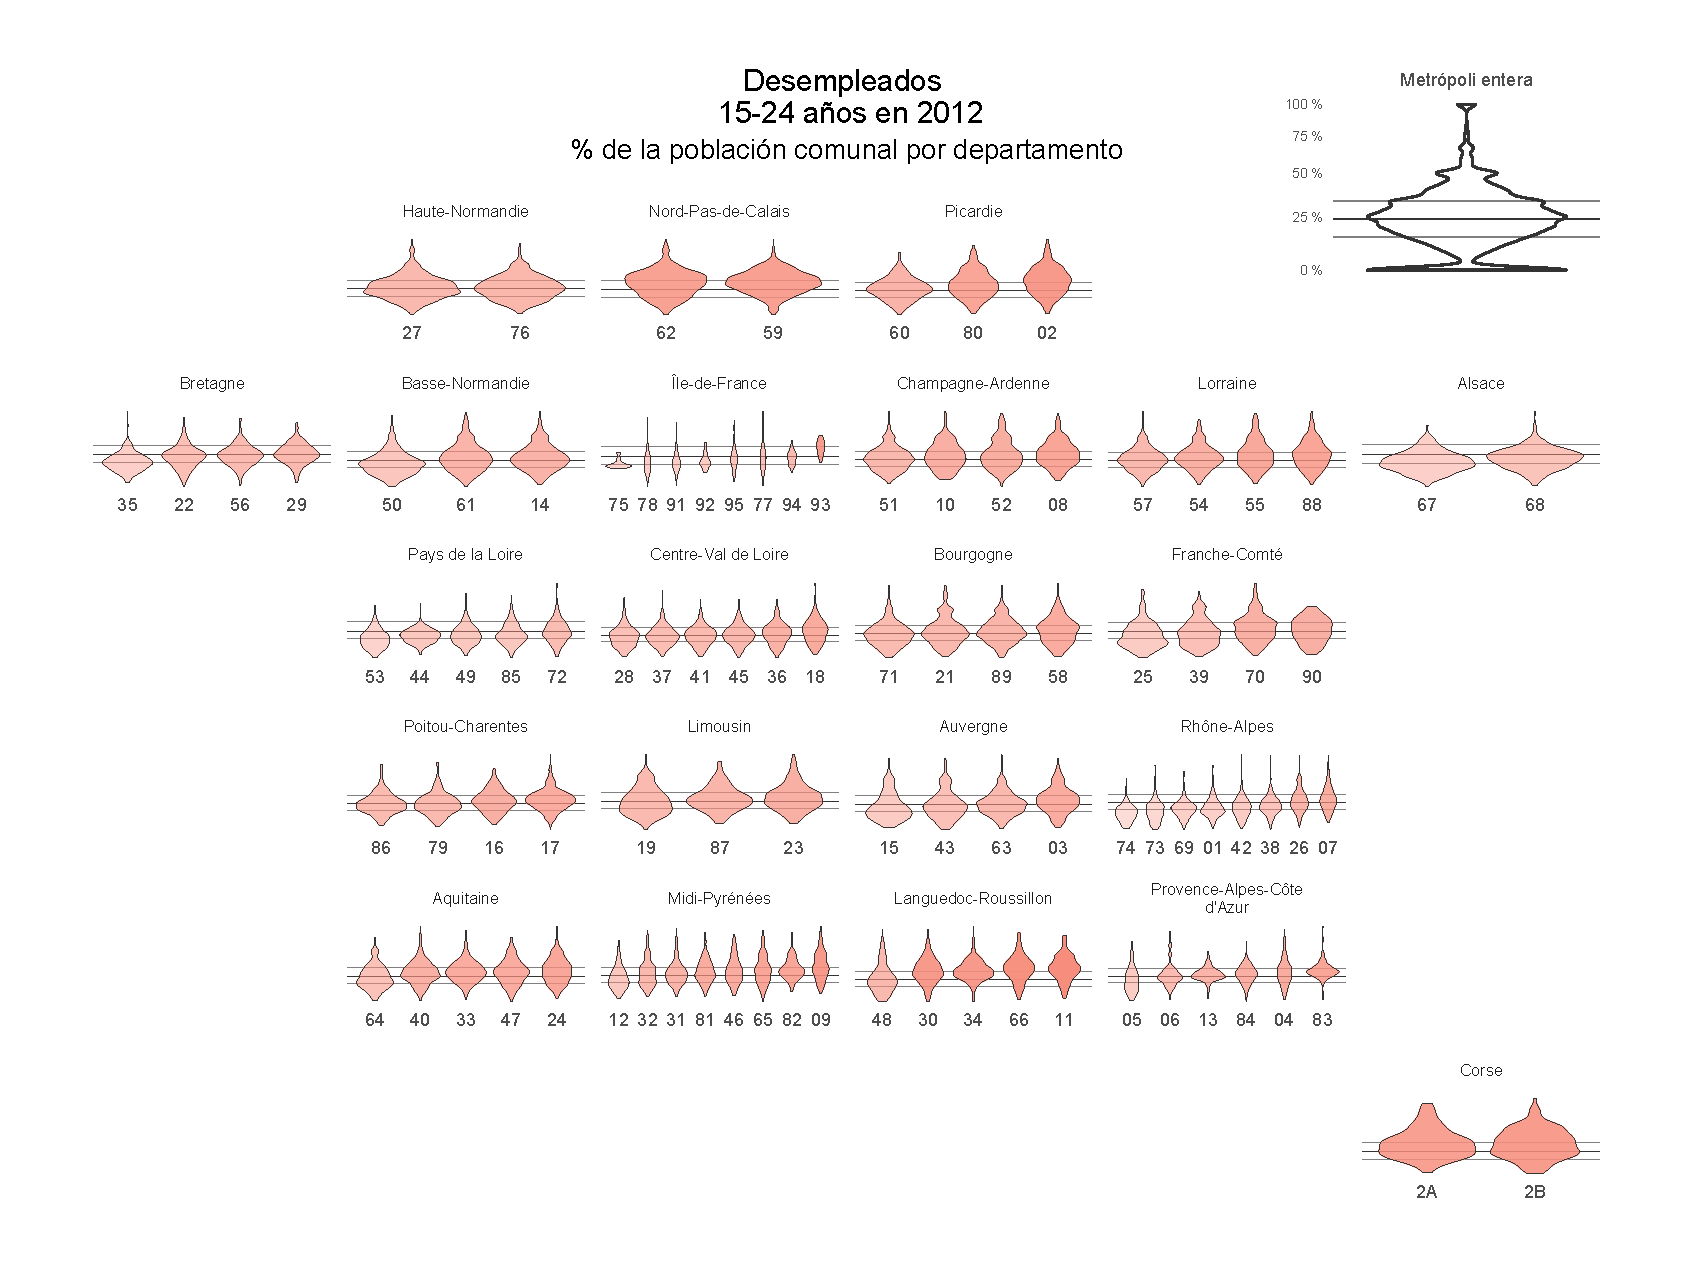
\includegraphics[width = \textwidth]{Figs/AED/Geofacet_Distr_por_Dpto_Des1_2012}
	\end{subfigure}
	~
	\begin{subfigure}{0.3\textwidth}
	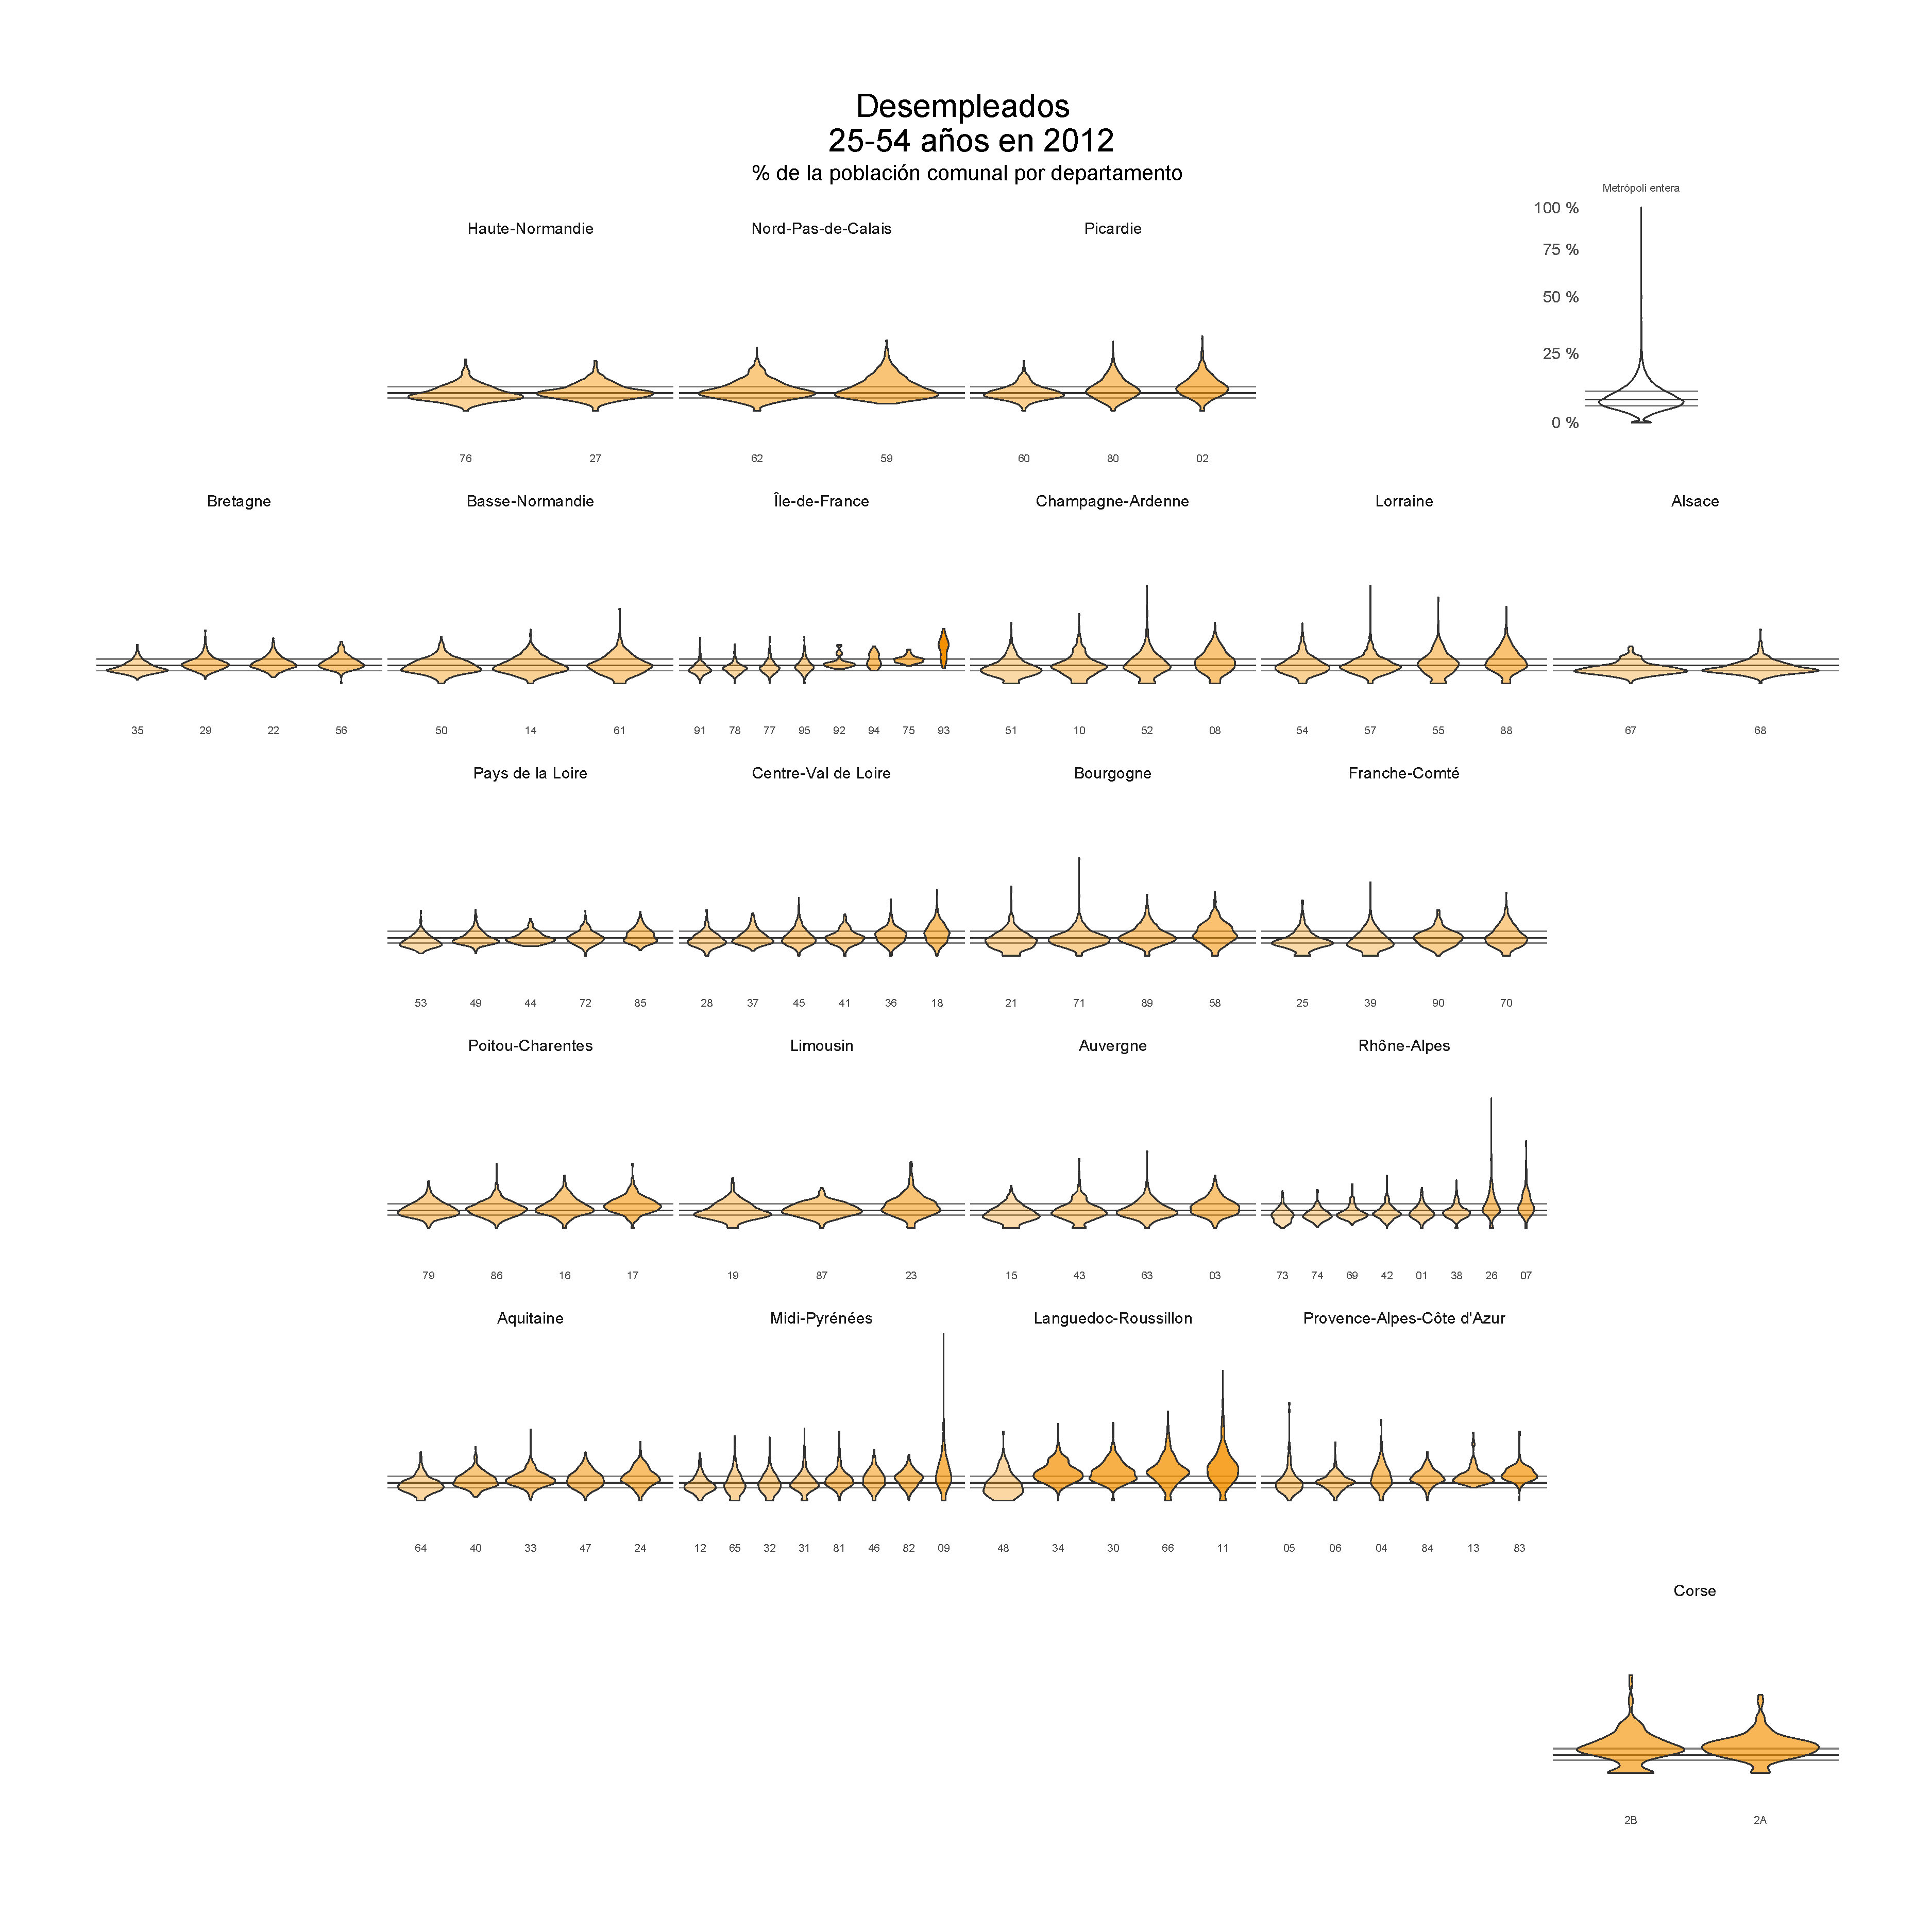
\includegraphics[width = \textwidth]{Figs/AED/Geofacet_Distr_por_Dpto_Des2_2012}
	\end{subfigure}~
	\begin{subfigure}{0.3\textwidth}
	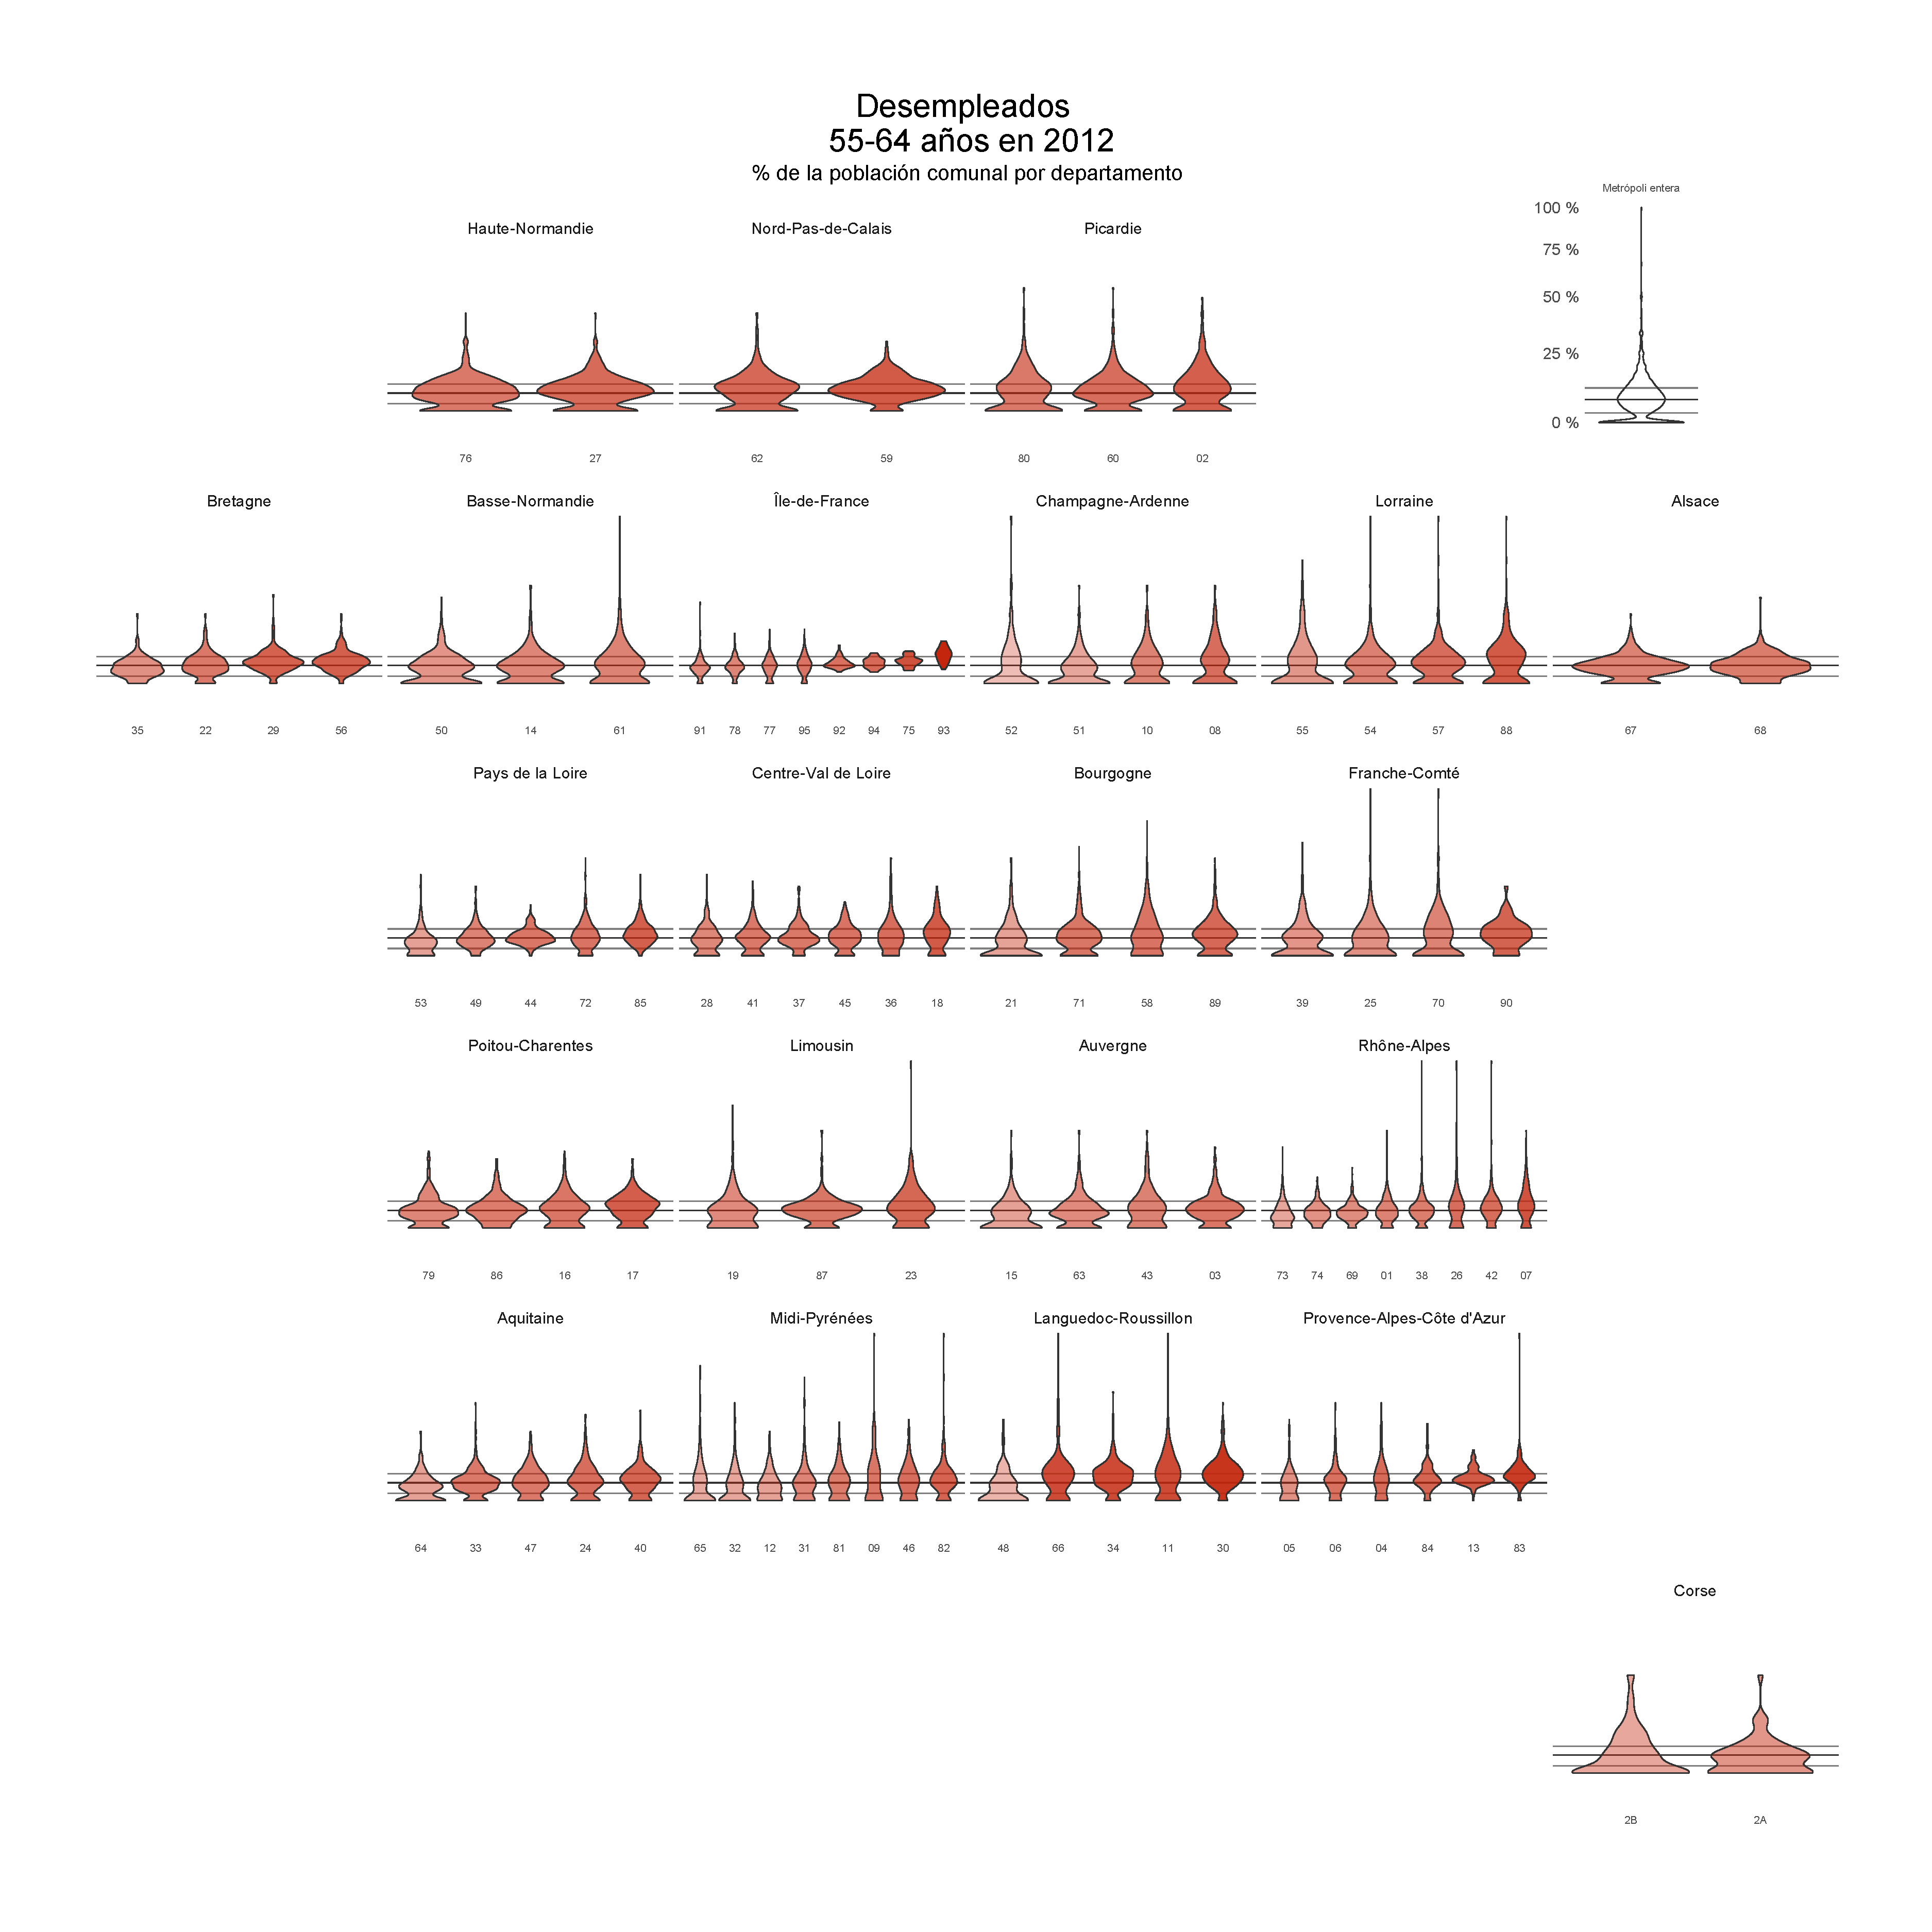
\includegraphics[width = \textwidth]{Figs/AED/Geofacet_Distr_por_Dpto_Des3_2012}
	\end{subfigure}
	\caption{Distribuciones departamentales de los porcentajes de desempleados en 2012. Fuente: elaboración propia con los datos del INSEE.}
	\label{fig:Distr_por_Dpto_Ocu_2012}	
\end{figure}

Para el desempleo general, 25 a 54 años, las distribuciones son más homogéneas. Notamos algunos casos por encima de la referencia nacional como el popular 93-Seine-Saint-Denis o los departamentos sureños del Languedoc-Rousillon o Corse. En el desempleo de adultos cercanos al retiro, 55-64 años, las distribuciones son mucho más sesgadas a la derecha con algunas colas largas. 

\section{Muestra de comunas}\label{secc:muestra}

En el proceso de modelado del siguiente capítulo se discutirán una serie de modelos. Debido al costo computacional que implica trabajar con poco más de 36,000 comunas, decidí seleccionar una muestra aleatoria de ellas para poder ajustar los modelos. Esta es una práctica recomendada cuando se intentarán explorar varios modelos con el objetivo de ir entendiendo de mejor manera el problema \parencite{GelmanHill06}. Después de algunas pruebas--- tomando en cuenta tanto el tiempo de ajuste como la precisión esperada dado el tamaño de muestra--- decidí que muestrear al rededor de 4,000 comunas era adecuado. Debido a que el análisis exploratorio discutido hasta ahora comienza a sugerir un modelado jerárquico de los datos a nivel departamento, el diseño de muestreo considerado es estratificado por departamento.\\ 

París y su pequeña corona--- departamentos 75, 92, 93 y 94--- están conformados por pocas comunas. En efecto, de entre estos, el de mayor número de comunas era el 94-Val-de-Marne, con 46, mientras que del resto de departamentos el que menos comunas tenía era el 90-Territoire de Belfort con 101. Esta diferencia de más del doble motivó la decisión de que para estos 4 departamentos en lugar de muestrear se censaran.\\

Para el resto de departamentos se realizó un muestreo aleatorio simple de comunas con un tamaño de muestra proporcional al número de comunas. Sin embargo, como el departamento 75-París se censaría en sus 20 comunas\footnote{Recordemos que técnicamente París es al mismo tiempo un departamento y una sola comuna. Sin embargo, tanto los resultados electorales como los datos del INSEE se tienen para cada uno de los 20 \textit{arrondisements} en los que se divide. Por ello, cada uno de estos \textit{arrondisements} se consideró como si fueran una comuna. Esto se repitió para los \textit{arrondisements} de las ciudades de Lyon y de Marsella.}, otra consideración fue que el tamaño mínimo de muestra en cada departamento fuera de 20 comunas. En total entonces se obtuvo una muestra de 4,157 comunas. Tanto el listado de comunas como el script con el que se obtuvo la muestra están disponibles en el repositorio de Github de esta tesis.\\

En la \textbf{Figura \ref{fig:Compara_Distr_Muestra}} vemos un comparativo de las distribuciones de porcentajes brutos de votos para las comunas muestreadas y aquellas fuera de muestra. Vemos que la muestra cubre correctamente el rango de la distribución, sin embargo está más concentrada en el centro de la misma y no refleja de la mejor manera las colas, sobre todo la moda en 0 que sí presentan las comunas fuera de la muestra. Esto hay que tenerlo en cuenta pues probablemente las predicciones que hagan los modelos serán más concentradas hacia la media o mediana de la distribución nacional y fallarán para comunas con porcentajes observados extremos. Sin embargo, para efectos de construcción del modelo es un sacrificio que aceptamos. La muestra logra delinear las grandes zonas de fuerza y debilidad del FN como vemos en el mapa de la \textbf{Figura \ref{fig:Mapa_Comunas_Muestra}}.\\
 
\begin{figure}[h]
	\centering
	\begin{subfigure}{0.45\textwidth}
	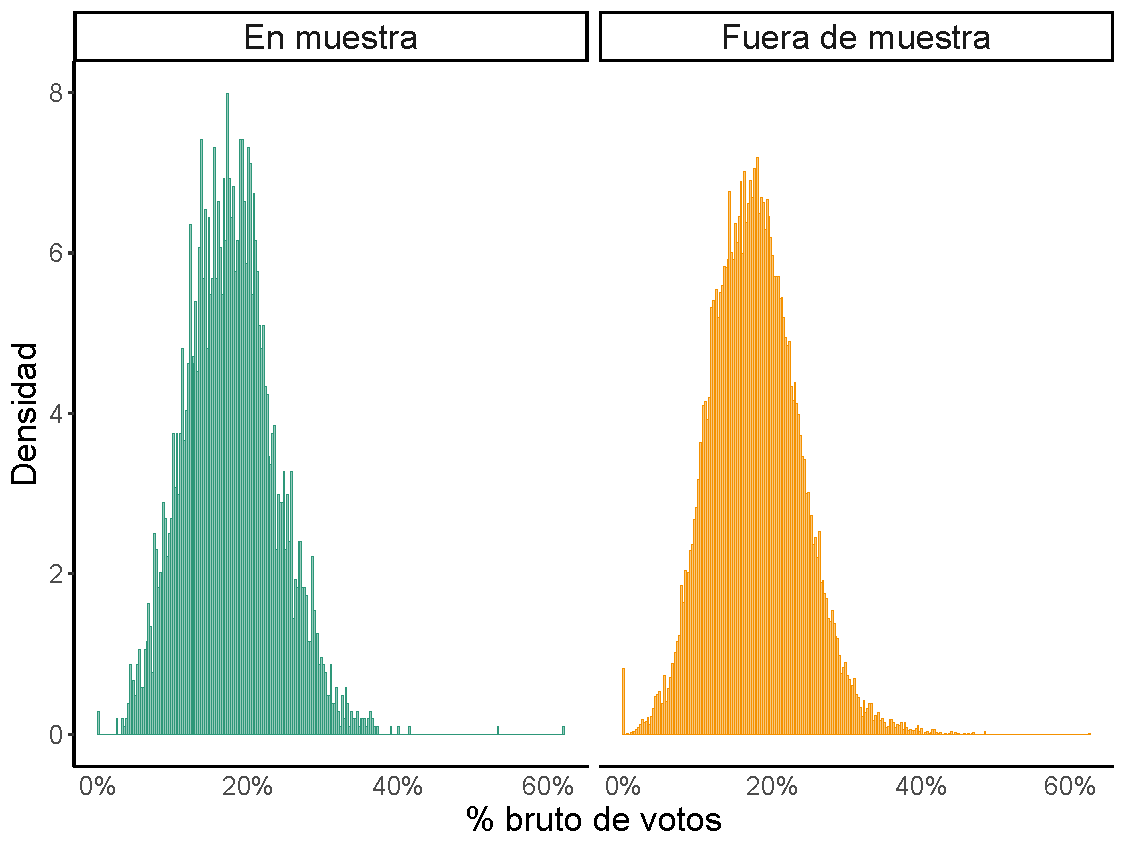
\includegraphics[width = \textwidth]{Figs/AED/Distr_Votos_Br_P12_FN_MUESTRA}
	\caption{}
	\label{fig:Compara_Distr_Muestra}		
	\end{subfigure}\\
	\begin{subfigure}{0.45\textwidth}
	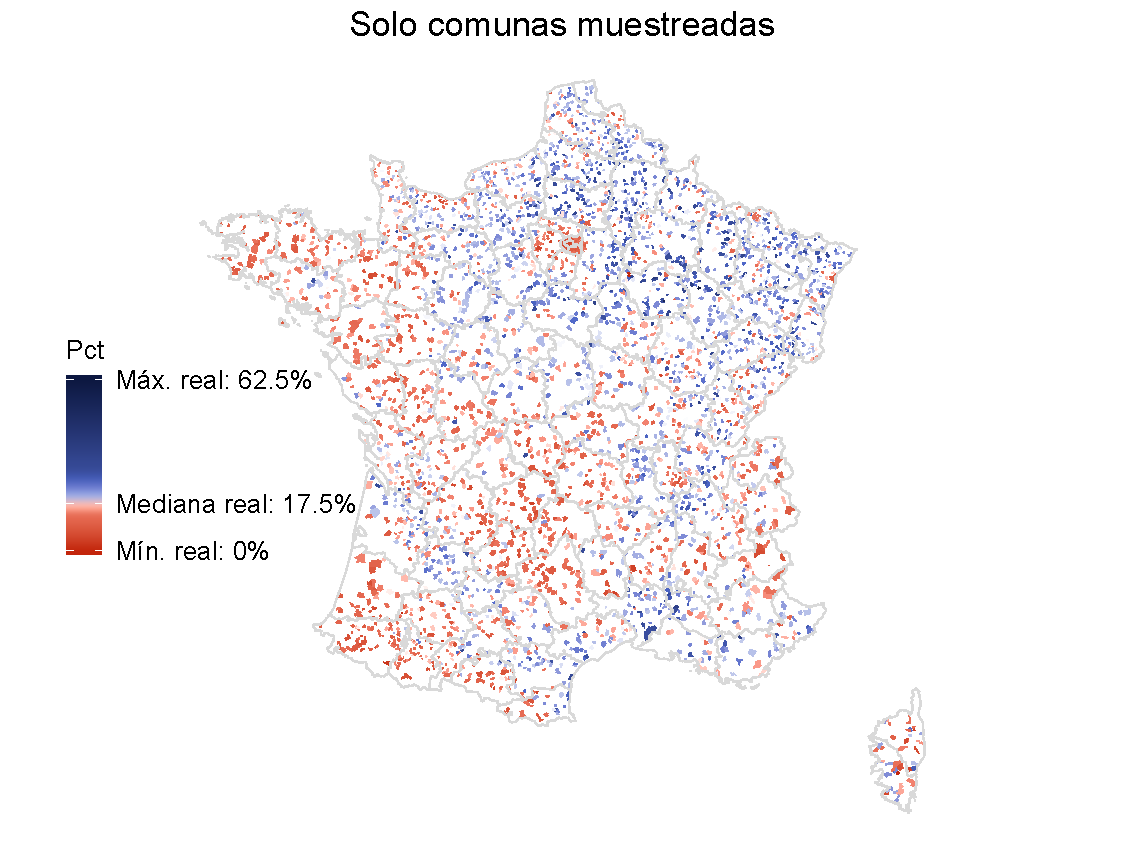
\includegraphics[width = \textwidth]{Figs/AED/Mapa_Votos_Br_P12_FN_MUESTRA}
	\caption{}
	\label{fig:Mapa_Comunas_Muestra}
	\end{subfigure}
	\caption{Distribuciones y mapa del \% bruto de votos para las comunas muestreadas. Fuente: elaboración propia con base en los datos electorales oficiales del Ministerio del Interior francés y la cartografía de OpenStreetMap.}
\end{figure}

Si estimáramos el porcentaje de votos en cada departamento con base en el porcentaje observado en la muestra, tendríamos errores de estimación que van de 0 puntos porcentuales (pp) para los departamentos censados hasta un máximo de 4.2 pp de error en el Bas-Rhin. 86 de los 96 departamentos tienen errores menores a 2.5 pp, lo que se observa por la mayoría de tonos rosas y morados en la \textbf{Figura \ref{fig:Errores_Est_Muestra}}. Este es un mapa \textit{dorling} en el que cada bolita representa un departamento, identificado con su código geográfico INSEE. Los departamentos que pertenecen a una misma región están unidos mediante las líneas grises. Así pues, podemos estar tranquilos de que la muestra ofrece una buena representación del fenómeno a nivel nacional.\\ 

\begin{figure}[h]
	\centering
	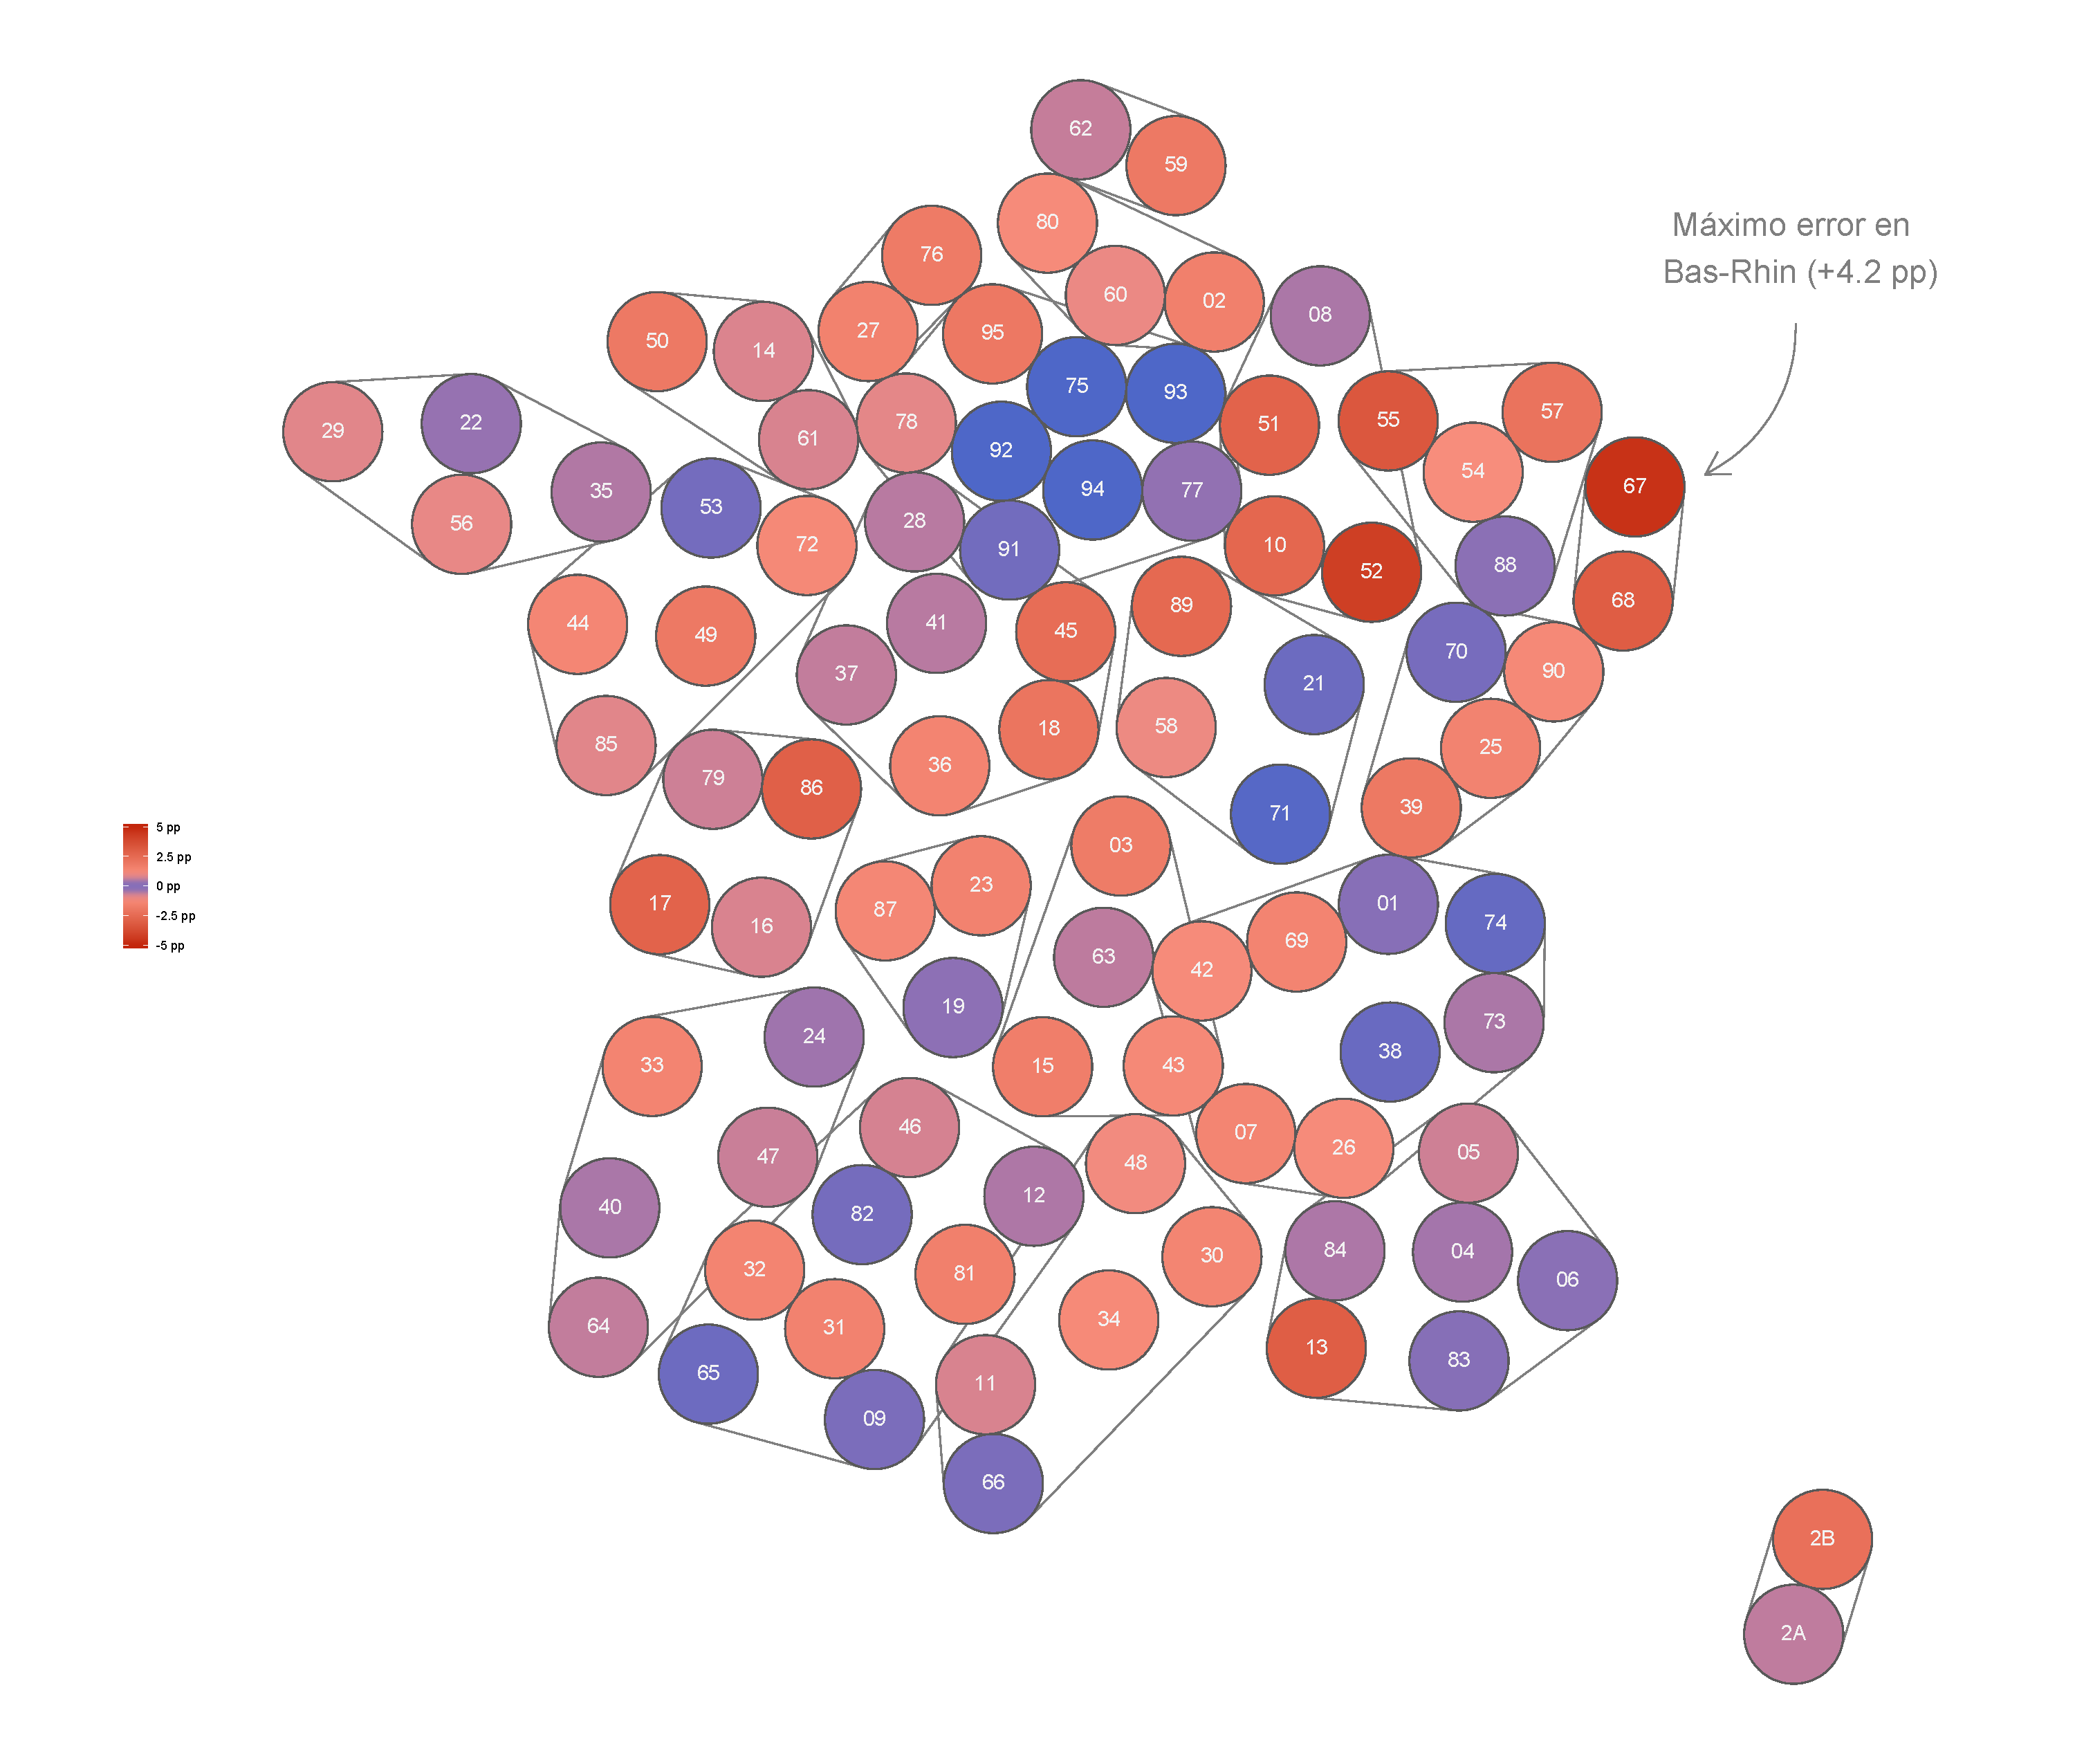
\includegraphics[width = 0.45\textwidth]{Figs/AED/Dorling_Errores_P12_FN_MUESTRA}
	\caption{Errores de estimación para cada departamento con base en la muestra. Fuente: elaboración propia.}
	\label{fig:Errores_Est_Muestra}	
\end{figure}

\section{Asociaciones}

Con esta muestra podemos explorar las asociaciones entre el voto y las configuraciones sociales definidas por las variables seleccionadas. Debido a que los datos que tenemos son tanto los votos obtenidos como el número de inscritos, es decir el máximo de posibles votos, una buena alternativa de modelado será considerar los datos como binomiales, donde nuestro parámetro de interés es el porcentaje bruto de votos obtenido por el FN, explicado por las configuraciones sociales. Por tanto, en lugar de intentar una asociación directa, podemos buscarla en la escala logística.\\

En la \textbf{Figura \ref{fig:Disper_Voto_Variables}} observamos diagramas de dispersión de los porcentajes brutos de votos observados en la escala logística\footnote{Cuando los porcentajes observados son iguales a 0, la transformación logística no está definida por lo que los puntos son representados como si estuvieran por debajo de cualquier otro valor en el eje vertical. Recordemos que el modelo binomial sí permite una cantidad nula de votos, es solo el logit de un parámetro de probabilidad de éxito igual a 0 lo que no estaría definido.} con respecto a los distintos porcentajes de la población que representa cada categoría de las variables explicativas. Cuando las categorías son dicotómicas, como el caso del sexo, solo se presenta una de las dos.\\ 

\begin{sidewaysfigure}
	\centering
	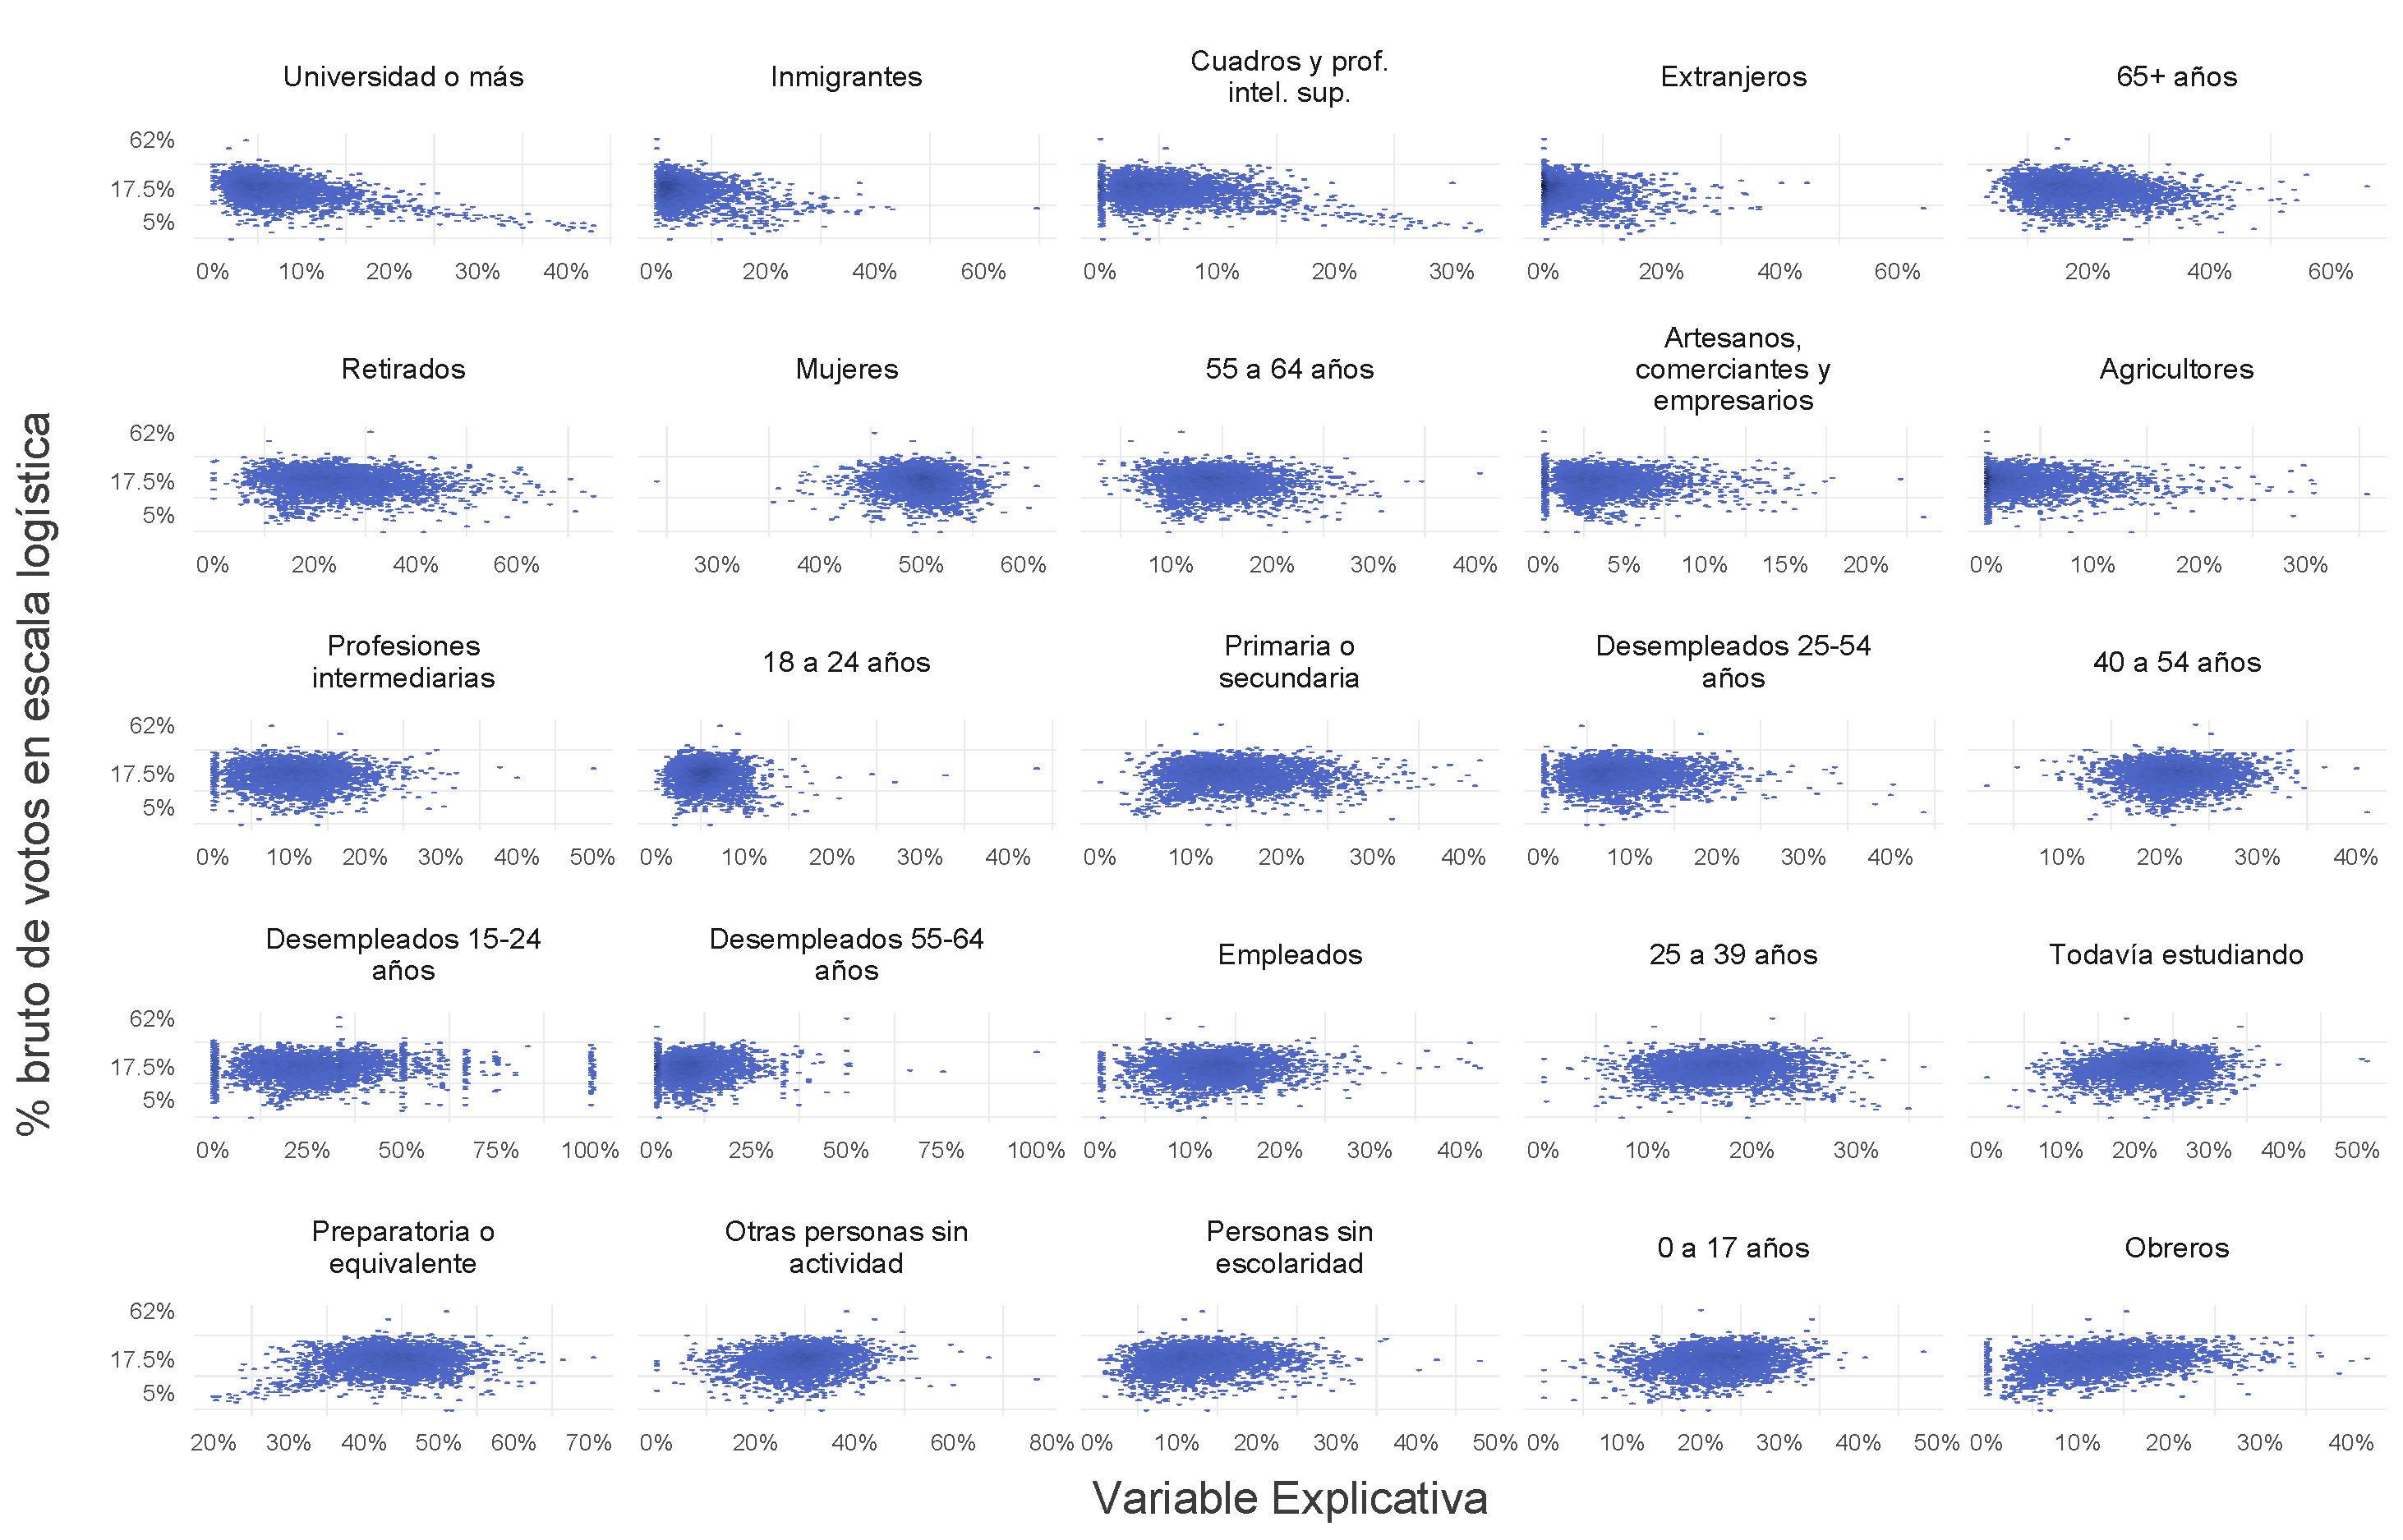
\includegraphics[width = 0.9\textwidth]{Figs/AED/Asociaciones_MUESTRA}
	\caption{Diagramas de dispersión para el logit de los porcentajes brutos de voto y las distintas variables explicativas observados en la muestra de comunas. Fuente: elaboración propia.}
	\label{fig:Disper_Voto_Variables}	
\end{sidewaysfigure}

Vemos que varias de las categorías presentan patrones de asociación tanto negativa--- Mujeres, Extranjeros, Inmigrantes, Universidad o más--- como positiva--- 0 a 17 años, Obreros---. También observamos que las variables explicativas presentan observaciones en 0 que dificultan a primera vista la asignación de una tendencia.\\

Ahora bien, estas nubes de puntos son para el conjunto de la muestra. Debido a que el fenómeno electoral es variable por departamento, podríamos preguntarnos si existen distintas asociaciones a través de los diferentes departamentos. En caso de existir diferencias, esperaríamos que un modelado jerárquico de los datos fuera una mejor alternativa que un modelo de agregación completa. Para explorar esta hipótesis presento los gráficos de la \textbf{Figura \ref{fig:Tendencias_Ingenuas_Muestra}} que llamo tendencias ingenuas con el objetivo de reafirmar que este es solamente un análisis exploratorio y no concluyente. Mediante el comando \verb|ggplot2::geom_smooth()| en $\mathsf{R}$, podemos ajustar tendencias lineales a todos los datos de la muestra que no hayan presentado un porcentaje de votos igual a 0. Estas son las lineas azules gruesas. Asimismo podemos realizar el ajuste para cada departamento, obteniendo las 96 líneas delgadas en color rosa.\\ 

\begin{sidewaysfigure}
	\centering
	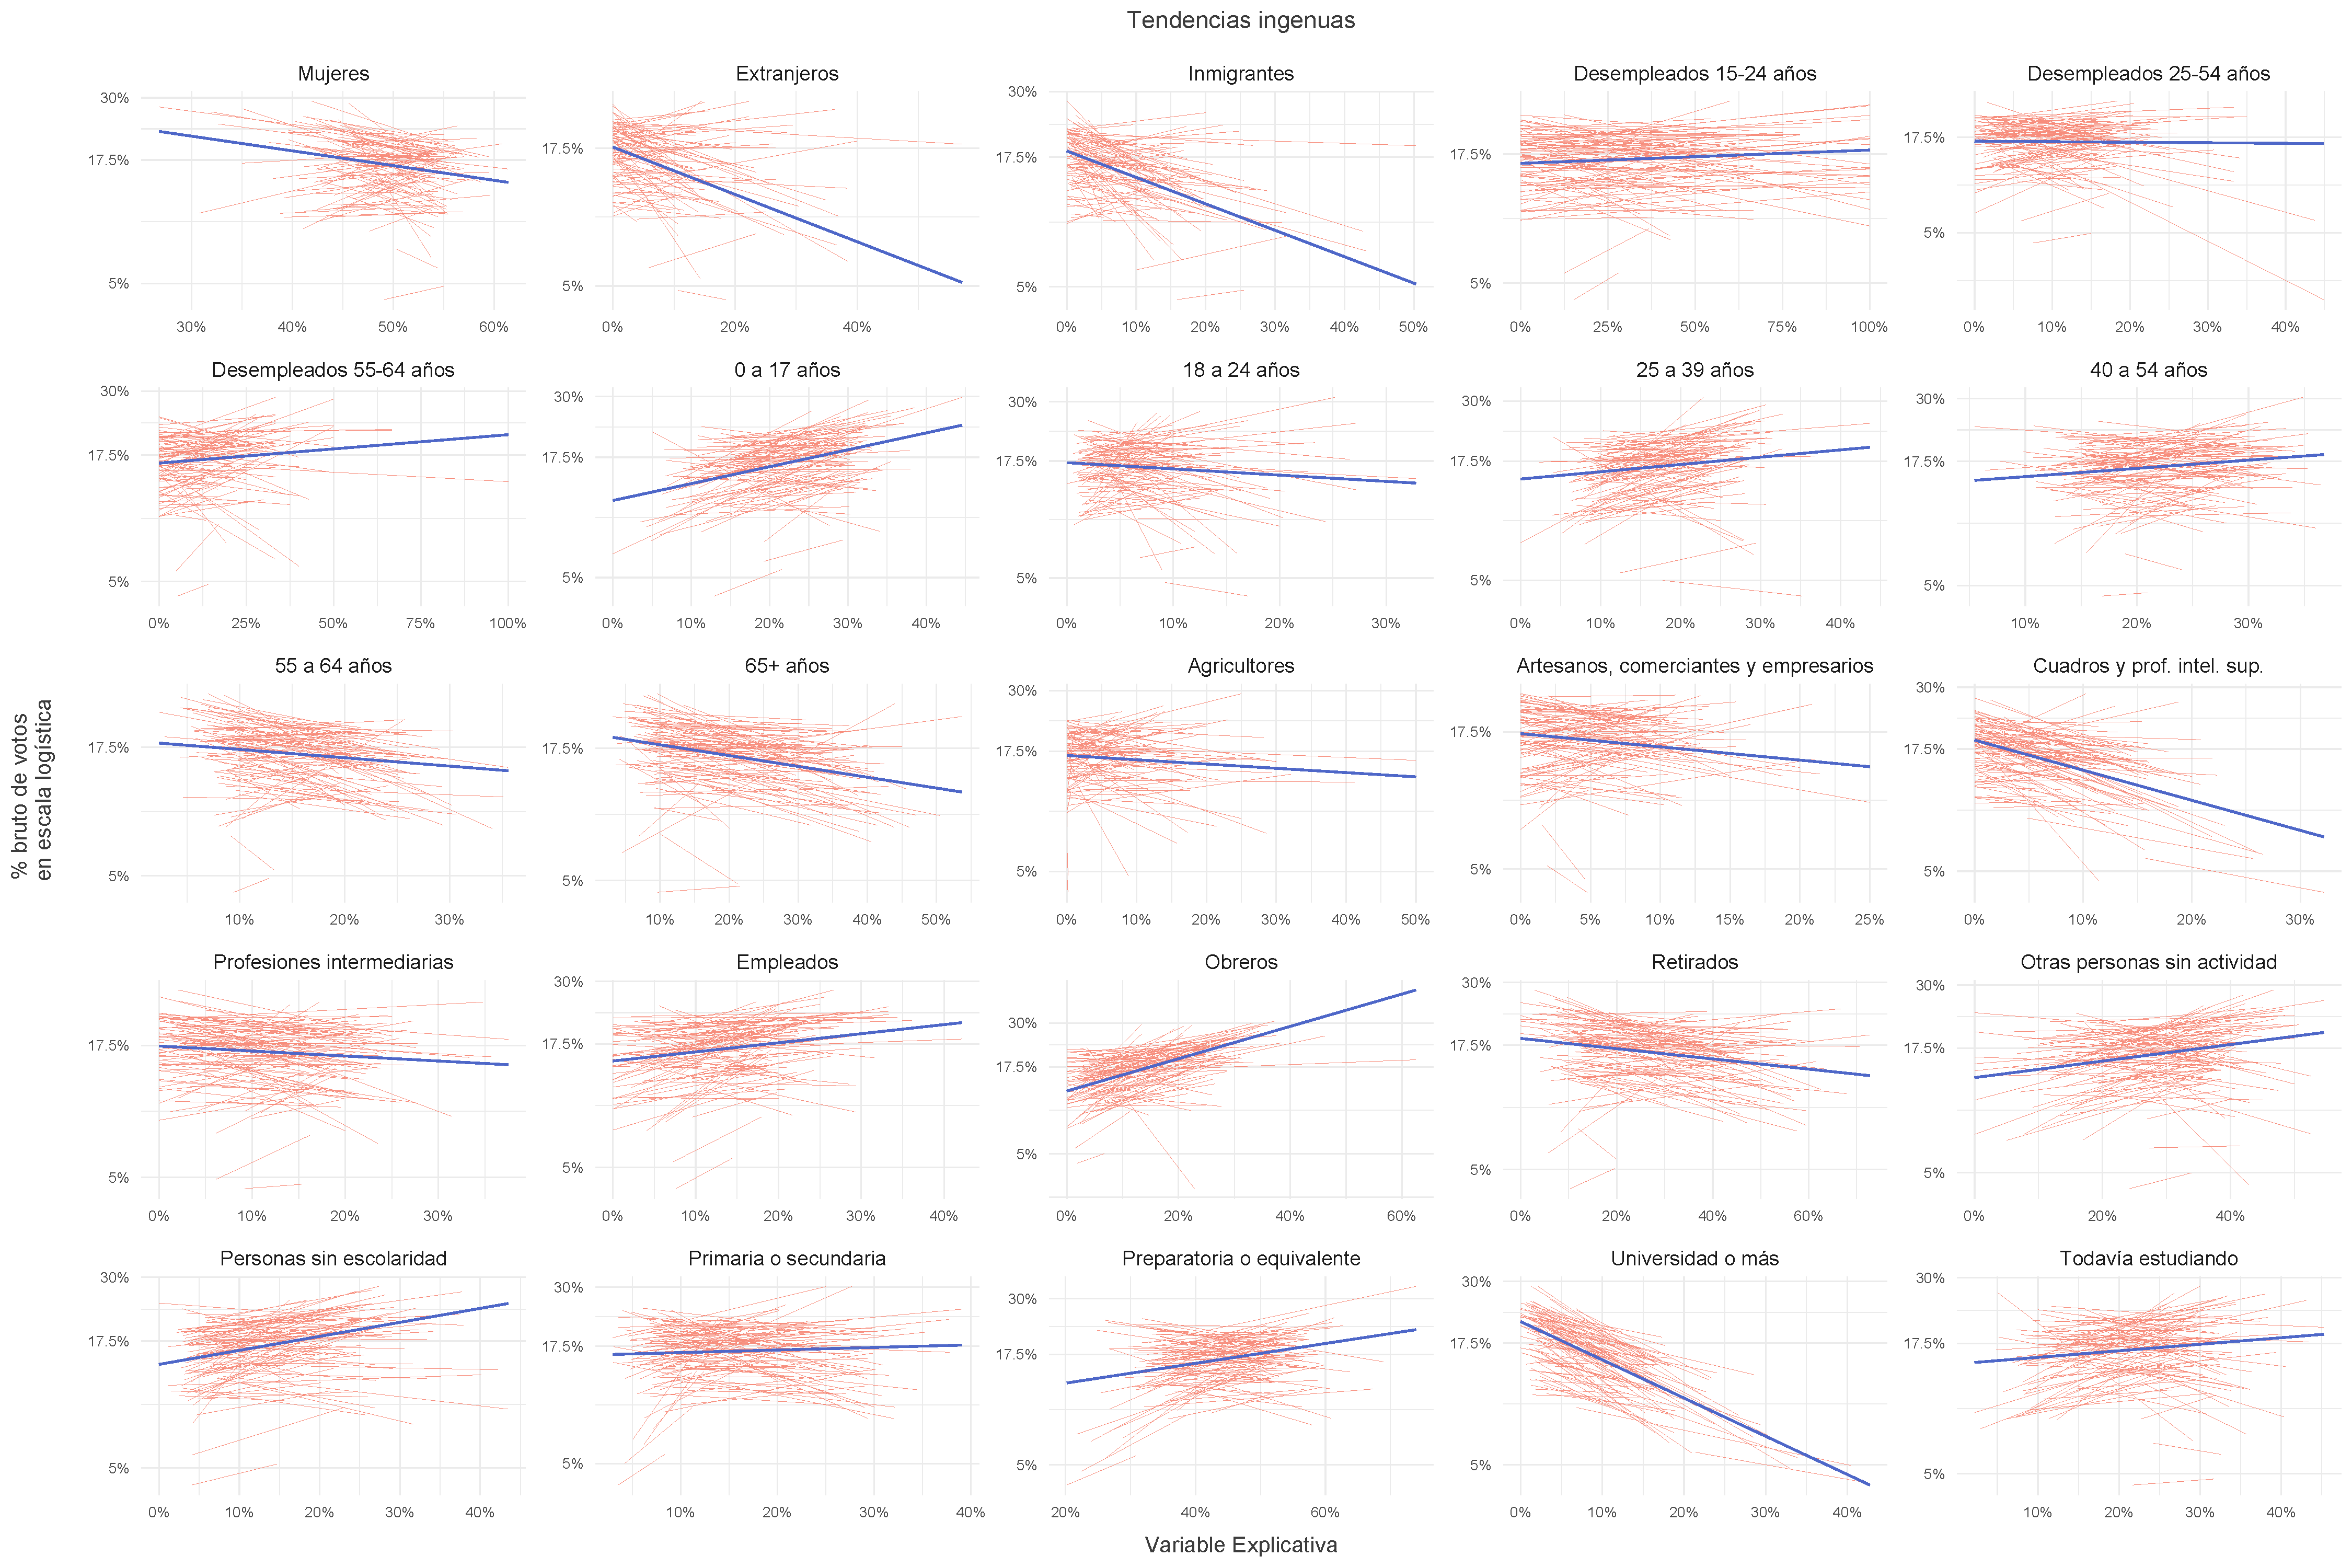
\includegraphics[width = 0.9\textwidth]{Figs/AED/Tend_Ingenuas_Todas_MUESTRA}
	\caption{Tendencias ingenuas para la muestra entera y por departamento calculadas mediante ajustes lineales en la escala logística. Fuente: elaboración propia.}
	\label{fig:Tendencias_Ingenuas_Muestra}	
\end{sidewaysfigure}

Efectivamente reafirmamos los indicios de asociaciones negativas para las categorías de Mujeres, Extranjeros, Inmigrantes y personas con diploma universitario. Pero también observamos pendientes ligeramente negativas para los grupos de edades 18 a 24, 55 a 64 y más de 65 años. Algunas categorías socioprofesionales como agricultores, artesanos, comerciantes y empresarios, cuadros y profesiones intelectuales superiores, profesiones intermediarias y retirados parecen tener también asociaciones negativas. Salvo quizás los casos del desempleo juvenil (15-24 años) y general (25-54 años) o las personas con primaria y secundaria, el resto de las categorías muestran tendencias positivas.\\

Ahora bien, las tendencias generales no son homogéneas a través de los departamentos. Las líneas rosas muestran una gran variabilidad tanto en términos de interceptos como de pendientes. Por ejemplo, aunque los desempleados de entre 25 y 54 años parecerían no tener ninguna relación tomando en cuenta todas las comunas, observamos algunas líneas rosas con claras pendientes. Quizás la categoría poblacional que muestra el comportamiento más homogéneo a través de los departamentos sea la población altamente escolarizada con diplomas de universidad y más--- última final y penúltima columna de la \textbf{Figura \ref{fig:Tendencias_Ingenuas_Muestra}}---.\\

Otro punto importante a notar es que estas tendencias ingenuas solamente se grafican para los rangos observados de los datos. Es decir, no se extrapolan las tendencias para todo el intervalo $[0,1]$. Esto es importante mencionarlo porque a la hora de analizar los modelos podría caerse en la tentación de querer predecir porcentajes de votos para valores de una categoría de alguna variable explicativa a lo largo de todo el intervalo. Extrapolar de esta manera es riesgoso y, además, podríamos caer en falacias si tomáramos el valor de $1$--- es decir toda la población comunal perteneciente a la misma categoría---. Por ejemplo, tendríamos situaciones ilógicas como hablar de votación emitida por individuos sin derecho al voto como los menores de edad o los extranjeros. No debemos perder de vista que el objetivo del análisis es la identificación de \textit{configuraciones sociales} que favorecieron el voto, no la inferencia sobre qué individuos emitieron los sufragios.\label{No_Extrapolar}\\

Con este análisis exploratorio en mente, procedo a modelar los datos electorales franceses de 2012 mediante regresiones binomiales con liga logística con la hipótesis de que se obtendrían mejores resultados con una estrategia jerárquica en lugar de agregación completa de los datos. 

